\chapter{Baseline/Non-adapted Cases}
\label{chapter:baseline_results}

%TODO: Move active camber to another chapter 

In this section, we focus on LES of flow over a surging airfoil at different conditions. Problem setup, and baseline results including vortex detection and tracking, are presented using the non-adapated mesh. We also present active flow control cases in the form of active reflex camber. 

\label{sec:baseline_results}

\section{Problem Setup: Surging Airfoils}
\label{sec:problem_setup_baseline}

A schematic of the problem setup is shown in Figure~\ref{fig:SetUpSketch}, where $U_\infty$ is the free-stream or mean velocity and $\alpha$ is the angle of attack.

\begin{figure}[H]
\centering
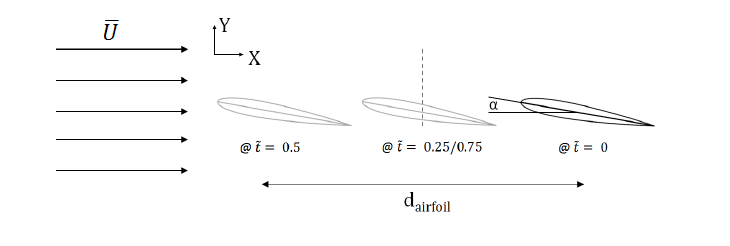
\includegraphics[width=0.8\textwidth]{figures/Setup/Setup.png}
\caption{Schematic of the problem}
\label{fig:SetUpSketch}
\end{figure}

The airfoil motion is set as follows
\begin{equation}
\label{eq:displacement}
  d_{airfoil} = A cos(2\pi f t) =  Acos(2\pi t/T) = Acos(2\pi\tilde{t})
\end{equation}

\noindent where $A$ is the amplitude and $T=1/f$ is the time period of the oscillation.
The variable $\tilde{t}$ is the fractional part in the oscillation cycle and is defined as $\tilde{t}=\{t/T\} = t/T - \lfloor t/T \rfloor$ (where $\lfloor \cdot \rfloor$ is the floor function).

The (non-dimensional) relative velocity is expressed as
\begin{equation}
\label{eq:relVelocity}
  \tilde{U}_{rel} = U_{rel}/U_\infty = 1 - U_{airfoil}/U_\infty = (1+\mu_{sect} sin(2\pi\tilde{t}))
\end{equation}
\noindent where $\mu_{sect}$ is the sectional advance ratio.
Note that for an advance ratio above $1.0$ a negative relative velocity or a reversed flow condition is attained.
Under this condition the relative flow is from the (geometric) trailing edge to the leading edge of the airfoil.

At $\tilde{t}$=0, with $\psi$=$0^\circ$ or $\psi$=$0^\circ$ (where, $\psi$ is the phase in the oscillation cycle and $\psi$ is the azimuthal position of the blade), the relative velocity is the free-stream velocity (i.e., $U_\infty$).
The same holds at $\tilde{t}$=0.5 or $\psi$=$180^\circ$.
At $\tilde{t}$=0.25 or $\psi$=$90^\circ$, the airfoil is at the maximum relative velocity and at $\tilde{t}$=0.75 or $\psi$=$270^\circ$ is at the minimum relative velocity.
Advancing phase is defined between $\tilde{t}$=0 or $\psi$=$0^\circ$ and $\tilde{t}$=0.5 or $\psi$=$180^\circ$ while retreating phase is between $\tilde{t}$=0.5 or $\psi$=$180^\circ$ and $\tilde{t}$=1.0 or $\psi$=$360^\circ$ (or back to $\psi$=$0^\circ$).

The free-stream or mean Reynolds number is defined as $Re=U_\infty C/\nu$, where $C$ is the chord.
The reduced frequency is defined as $k=\pi f C/U_\infty$ while the amplitude is related as $A = \frac{\mu_{sect} C}{2k}$.

\section{Summary of Baseline Cases}
\label{sec:baseline_case_summary}

In the current study, the reduced frequency is held fixed at $k$=0.133 while three Reynolds numbers of $Re$=40,000, 200,000 and 1,000,000 are considered together with two advance ratios of $\mu_{sect}$=1.0 and 1.2, i.e., six cases are considered in total.
The angle of attack of the airfoil is set to 6$^\circ$.
Note that we considered the Reynolds number of $Re$=40,000 in previous study~\cite{bib:kocher_scitech2017} that was selected in accordance with the experiments conducted in \cite{bib:granlund2016} where the airfoil was placed in a constant flow and oscillated in the streamwise direction.
The six cases are summarized in Table~\ref{table:summary_cases}.

\begin{table}[H]
\centering
\caption{Summary of cases}
\label{table:summary_cases}
\begin{tabular}{|l|c|c|c|c|}
\hline
Airfoil   & $\alpha$ & $k$ & $\mu_{sect}$ & $Re$ \\
\hline
\hline
NACA 0012 & 6$^\circ$ & $0.133$ & \{1.0, 1.2\} & \{40,000,\; 200,000,\; 1,000,000\} \\
\hline
\end{tabular}
\end{table}

The computational domain is set to be $100C$ x $50C$ x $0.2C$.
At the inlet, a constant free-stream velocity is applied
(note that the airfoil is moved sinusoidally in the streamwise direction).
No-slip condition is prescribed on the moving airfoil.
The top and bottom surfaces are set as slip walls.
Side surfaces in the spanwise direction (i.e., front and back surfaces) are imposed to be periodic.
A natural pressure condition is used at the outlet.
A second-order implicit time integration scheme, e.g., see\cite{bib:tran2017b}, is employed with about 1,440 steps in an oscillation cycle.

%TODO: give justification for this mesh ... typical LES resolution for a BL (based on highest Reynolds number in the surge cycle) ... but indicate no consideration taken for other flow features such as separation and LEV.
An unstructured hybrid/boundary layer mesh is used.
The mesh is comprised of hex and wedge elements which is generated by first generating a mesh on the front surface and subsequently applying an extrusion in the spanwise direction. This mesh is used for all the baseline cases.
Refinement zones are placed around the airfoil to resolve the flow structures of interest, see Figure \ref{fig:mesh} (where three refinement zones are noted).
In the finest refinement zone (Z1), mesh size is set to be $C/256$.
In the subsequent two zones (Z2 and Z3), it is set to be $C/128$ and $C/64$, respectively.
In the spanwise direction, 50 extruded elements are used.
A layered and graded mesh (with geometric growth) is used around the airfoil surface, see Figure \ref{fig:mesh2}.
The first layer height is set to be $\mathcal{O}(10^{-5} C)$ such that it is below 1 in wall units for all cases.
Similarly, mesh spacing on the airfoil surface in the streamwise and spanwise directions is set to be below 80 and 50 in wall units, respectively.
Overall the mesh contains about 6.2 million nodes and 10.8 million elements.

\begin{figure}[H]
\centering
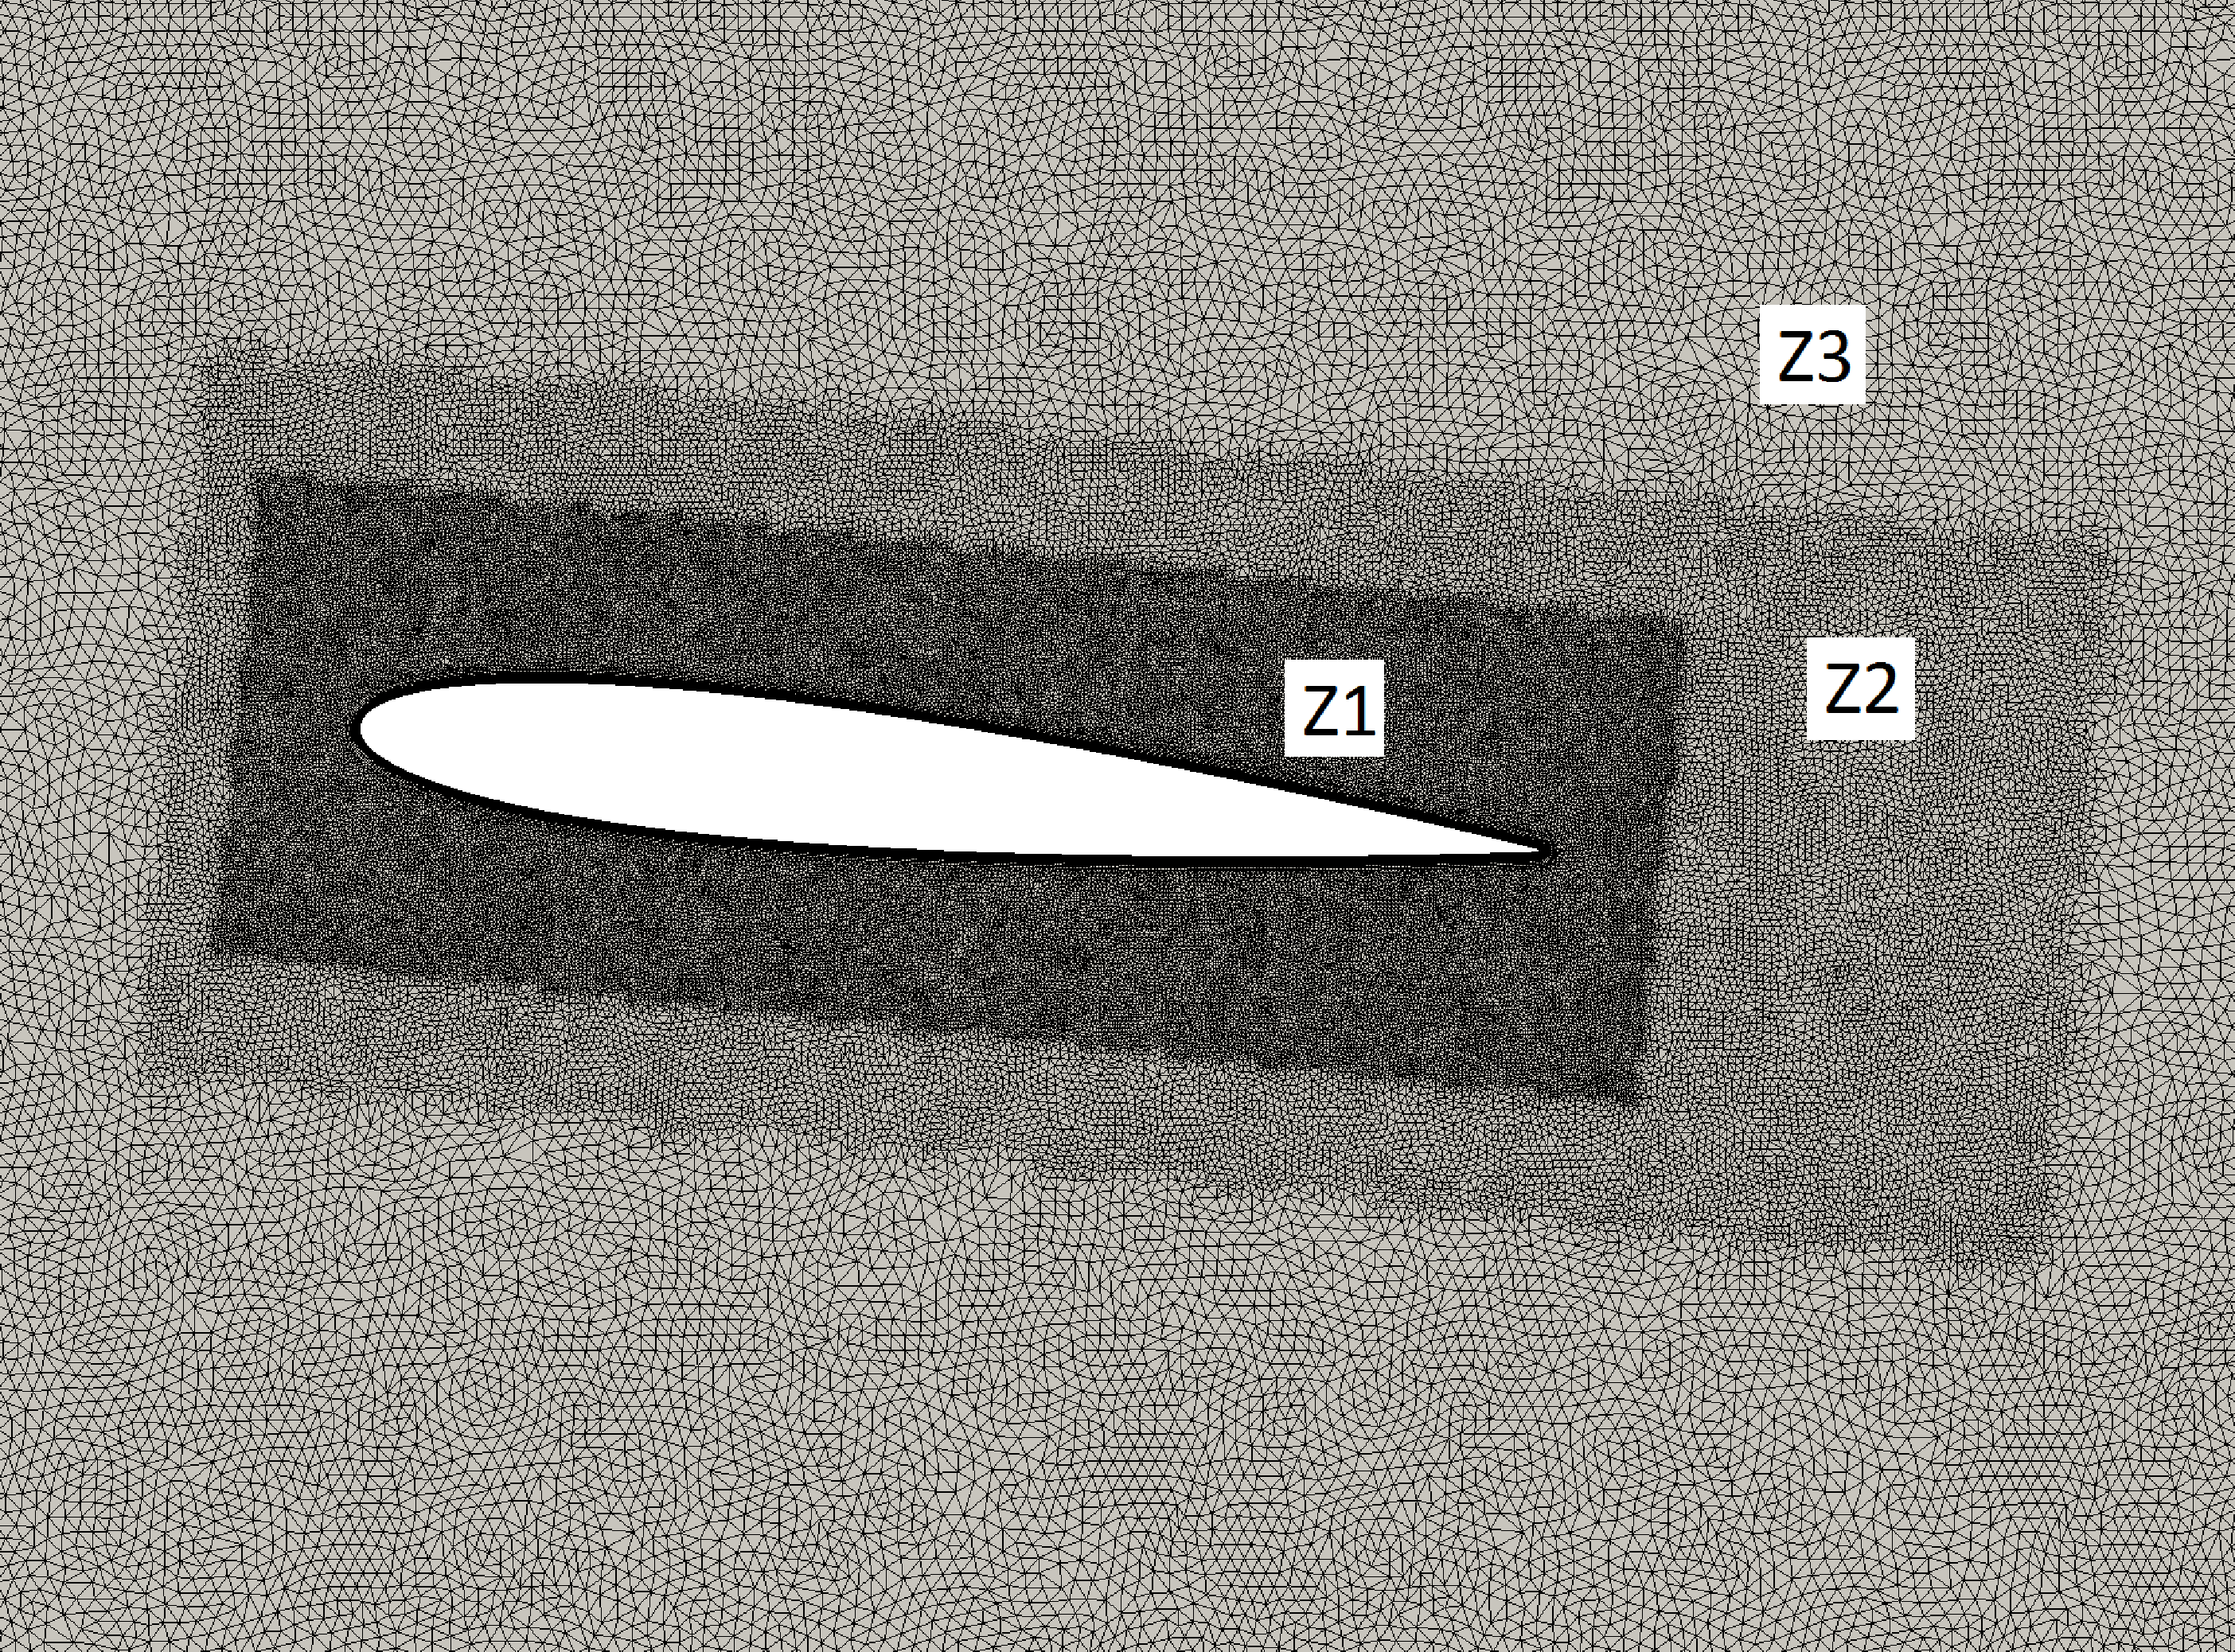
\includegraphics[width=0.7\textwidth]{figures/Setup/mesh_screenshot.pdf}
\caption{Mesh around the airfoil with refinement zones}
\label{fig:mesh}
\end{figure}

\begin{figure}[H]
\centering
\includegraphics[width=0.45\textwidth]{figures/Setup/mesh_LE.pdf}
\includegraphics[width=0.45\textwidth]{figures/Setup/mesh_TE.pdf}
\caption{Layered and graded mesh around the leading edge and trailing edge of the airfoil}
\label{fig:mesh2}
\end{figure}

\section{Results and Discussion}

\subsection{Force Response}

\begin{figure}[H]
	\begin{subfigure}{0.5\textwidth}
		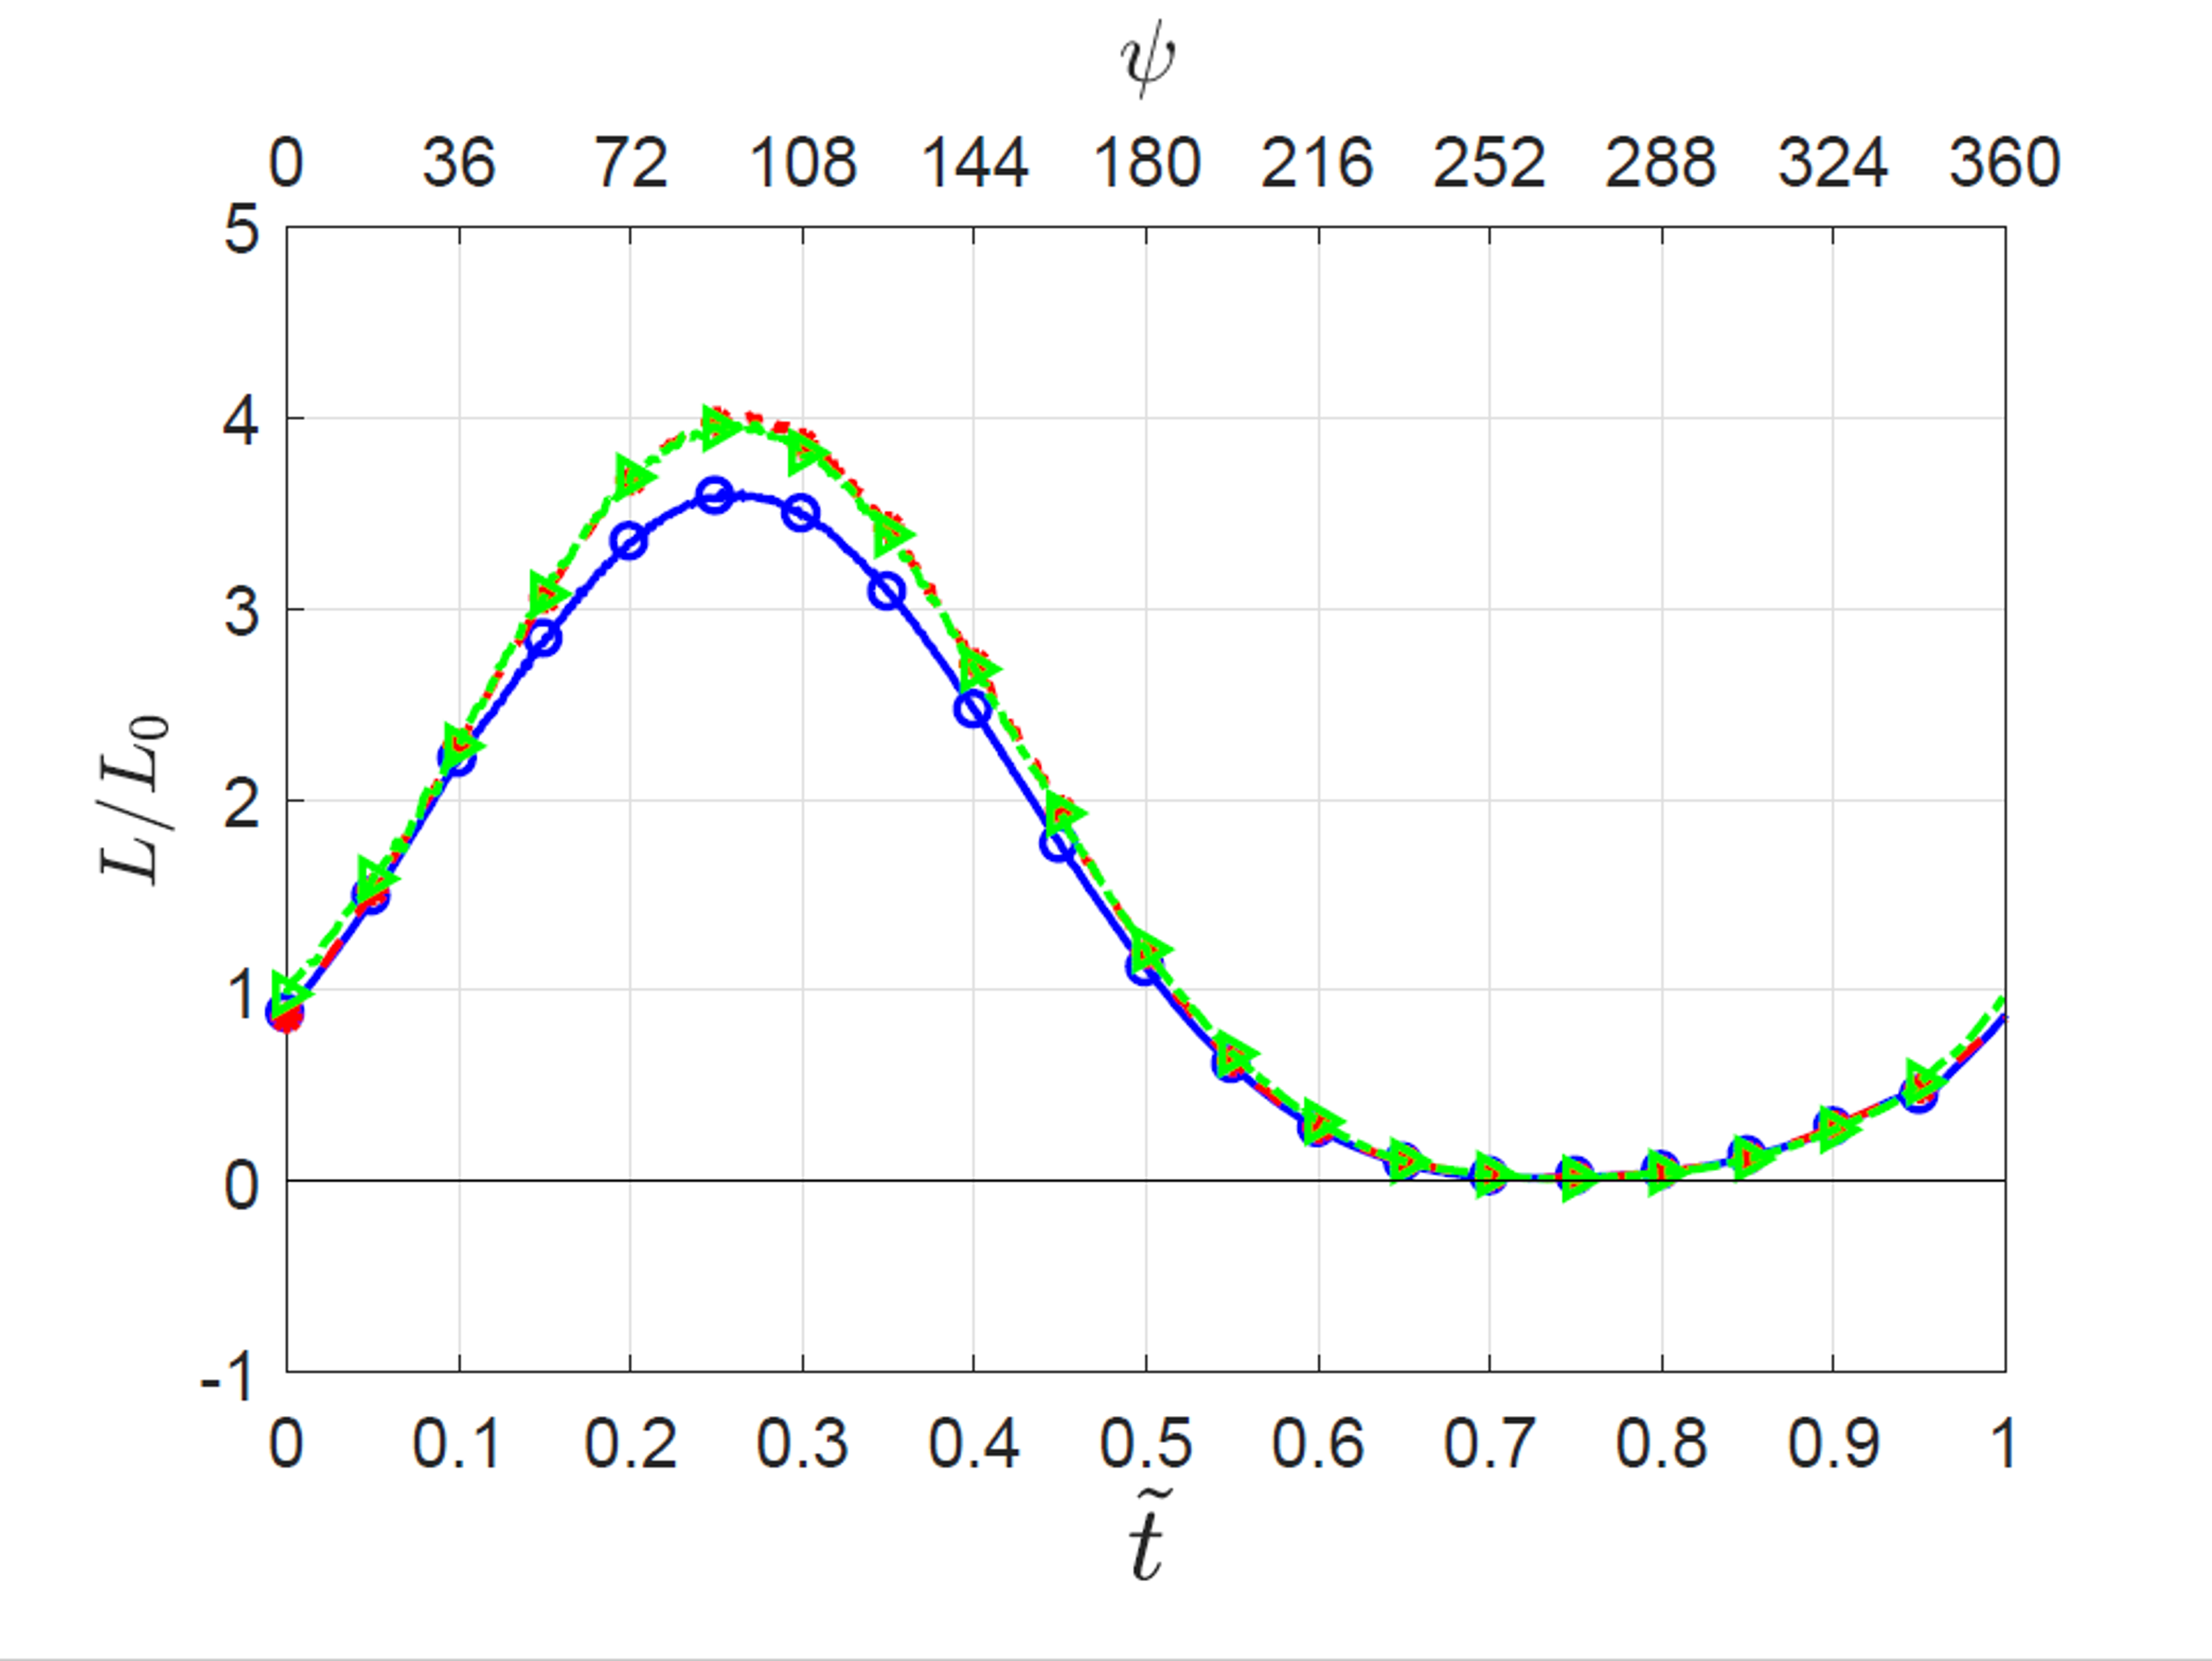
\includegraphics[width=1\textwidth]{figures/lift_Re_effect_lambda_1pt0.png}
		\subcaption{$\mu_{sect} = 1.0$}
		\label{fig:lift_Re_comparision_lambda_1p0}
	\end{subfigure}
 	\begin{subfigure}{0.5\textwidth}
		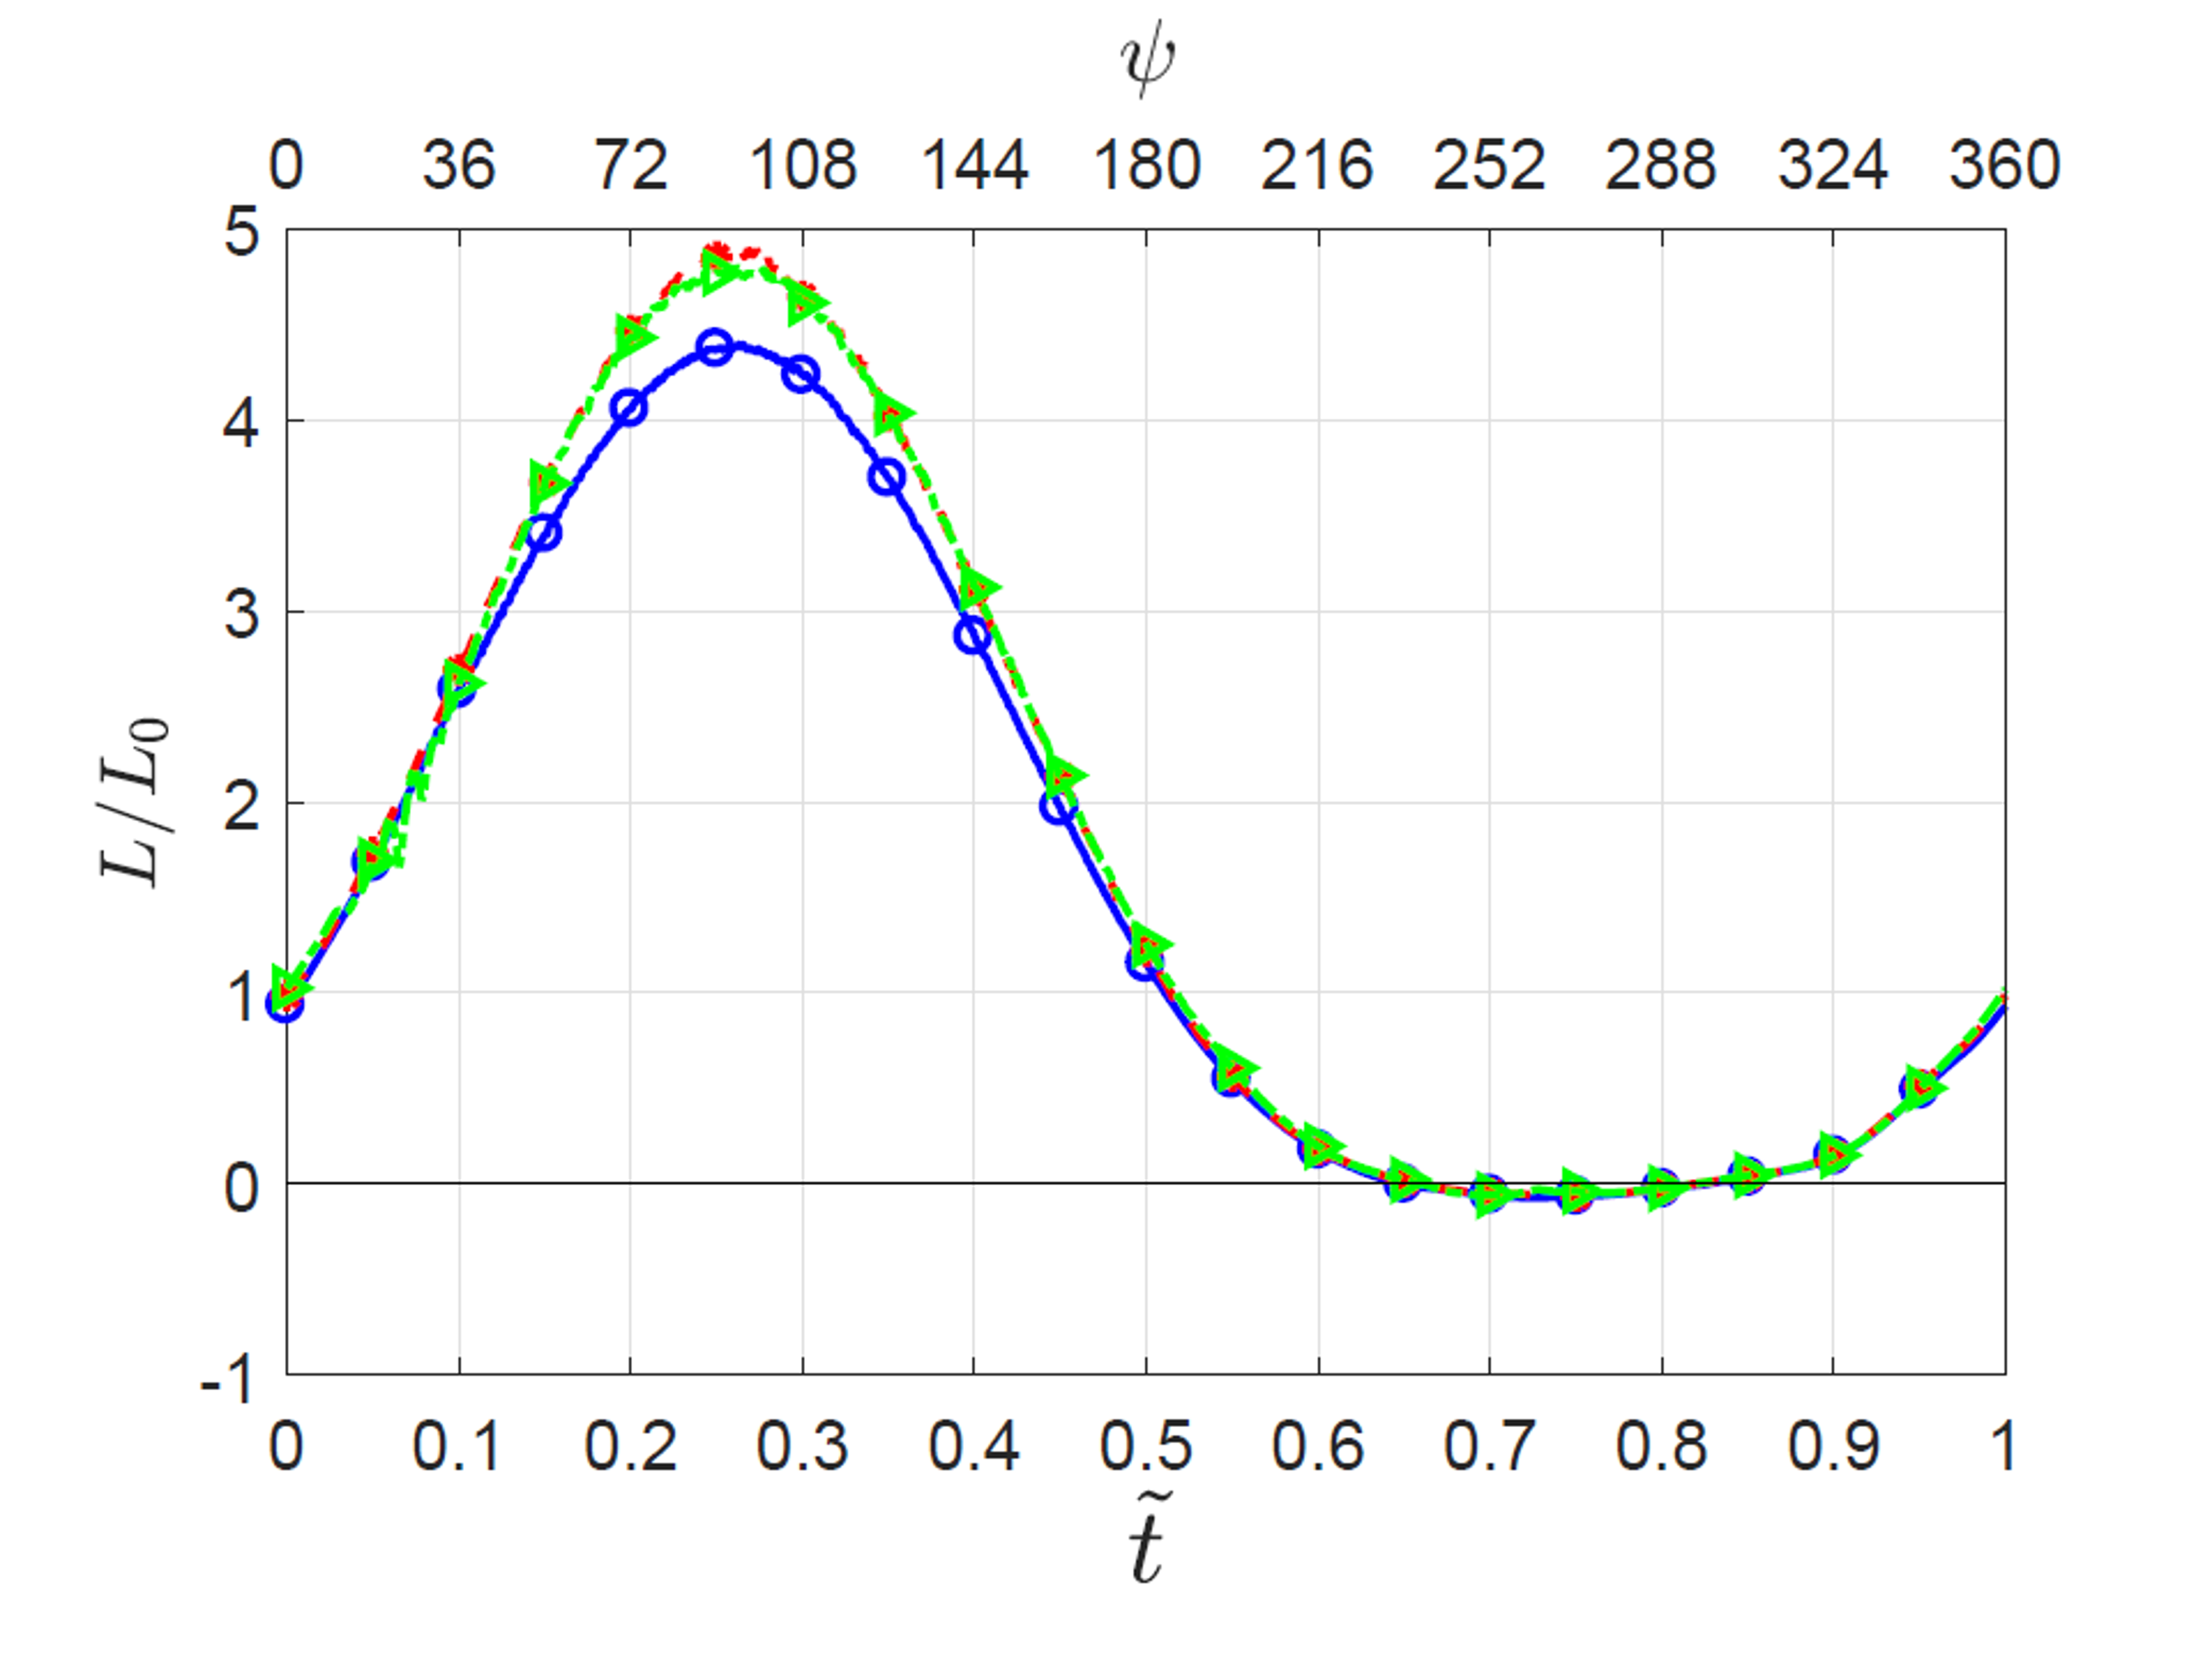
\includegraphics[width=1\textwidth]{figures/lift_Re_effect_lambda_1pt2.png}
        \subcaption{$\mu_{sect} = 1.2$}
		\label{fig:lift_Re_comparision_lambda_1p2}
	\end{subfigure}

 	\caption{Normalized lift force for $Re$=40,000 (green line with open triangles), 200,000 (red line with closed circles) and 1,000,000 (blue line with open circles) at $\mu_{sect}$=1.0 and 1.2}
 	\label{fig:lift_comparison}
\end{figure}

Lift force is shown in Figure \ref{fig:lift_comparison}.
Lift is normalized by its static counterpart, i.e., $L_0$ is the average or steady lift for the static airfoil at mean Reynolds number.
This normalization was used in our previous study with $Re$=40,000~\cite{bib:kocher_scitech2017} to compare against the experimental data of \cite{bib:granlund2016}, where a good agreement was shown between the experimental and simulation data.
As noted earlier, data is phase averaged over 4 cycles.
%%%We note that the averaged drag data exhibits fluctuations which is due to the presence of a turbulent flow, especially during the advancing phase of the cycle with a higher relative velocity or Reynolds number.
%%%However, these fluctuations are marginal in nature and averaging over additional cycles will be useful.

Overall, the lift force follows a similar qualitative trend for all the cases.
Maximum lift is achieved at $\tilde{t}=0.25$, which is expected as the airfoil achieves maximum relative velocity at that point.
After $\tilde{t}=0.25$, the lift starts decreasing as the airfoil begins to decelerate and enters the retreating phase. 
The lift keeps decreasing till about $\tilde{t}=0.65$ and plateaus or reaches a value close to zero during the middle of the retreating phase (i.e., around $\tilde{t}=0.75$ when the airfoil is at its minimum relative velocity).
We note that for both advance ratios of $\mu_{sect}$=1.0 and 1.2 a zero relative velocity is attained and for the higher advance ratio of $\mu_{sect}$=1.2 the relative velocity also becomes negative.
Lift starts to recover after $\tilde{t}=0.75$ as the airfoil starts accelerating again.
For each advance ratio, the normalized lift during the advancing phase for $Re$=1,000,000 is smaller compared to the other two Reynolds numbers, see Figure \ref{fig:lift_Re_comparision_lambda_1p0} or Figure \ref{fig:lift_Re_comparision_lambda_1p2}.
The normalized lift is very similar between $Re$=40,000 and 200,000 cases.
The peak normalized lift is about 9\% lower for the highest Reynolds number case as compared to the lower Reynolds number cases for each advance ratio.
On the other hand, for a given Reynolds number the normalized lift is higher for the higher advance ratio, which is expected due to the higher dynamic pressure in any given instance or phase in the surging cycle.
The peak normalized lift is about 21\% higher for the higher advance ratio case as compared to the lower advance ratio case for each Reynolds number, which is the difference in the peak dynamic pressure between the two advance ratios.

\subsection{Flowfield: Spanwise Vorticity}

In this section, we present spanwise vorticity over the cycle at 8 different phases of $\psi$ = $195^\circ$, $225^\circ$, $240^\circ$, $255^\circ$, $270^\circ$, $270^\circ$, $315^\circ$, $330^\circ$,and $345^\circ$, which are all in the retreating phase of the surging cycle.
We focus our attention on the LEV which is the dominant flow feature.
It forms and advects during the retreating phase while in the advancing phase the flow remains attached.
As noted earlier, data is phase averaged over 4 cycles.
In addition, averaging is also applied in the spanwise direction.

Figure \ref{fig:vortScreen_1pt0} shows the spanwise vorticity for the lower advance ratio of $\mu_{sect}$=1.0.
The voriticy range is selected to be [-10,10]$\times U_\infty /C$.
At $\psi$=$195^\circ$, the flow over the airfoil is mostly attached, however, the boundary layer is relatively thick as the airfoil is decelerating, see Figures~\ref{fig:Re_40k_1pt0_phi195}, \ref{fig:Re_200k_1pt0_phi195} and \ref{fig:Re_1m_1pt0_phi195}.
As expected, the boundary layer is much thicker for the lowest Reynolds number of $Re$=40,000 as compared to the other two higher Reynolds number.

\begin{figure}[H]
	\centering
	
	\begin{subfigure}[b]{0.32\textwidth}
		\centering
		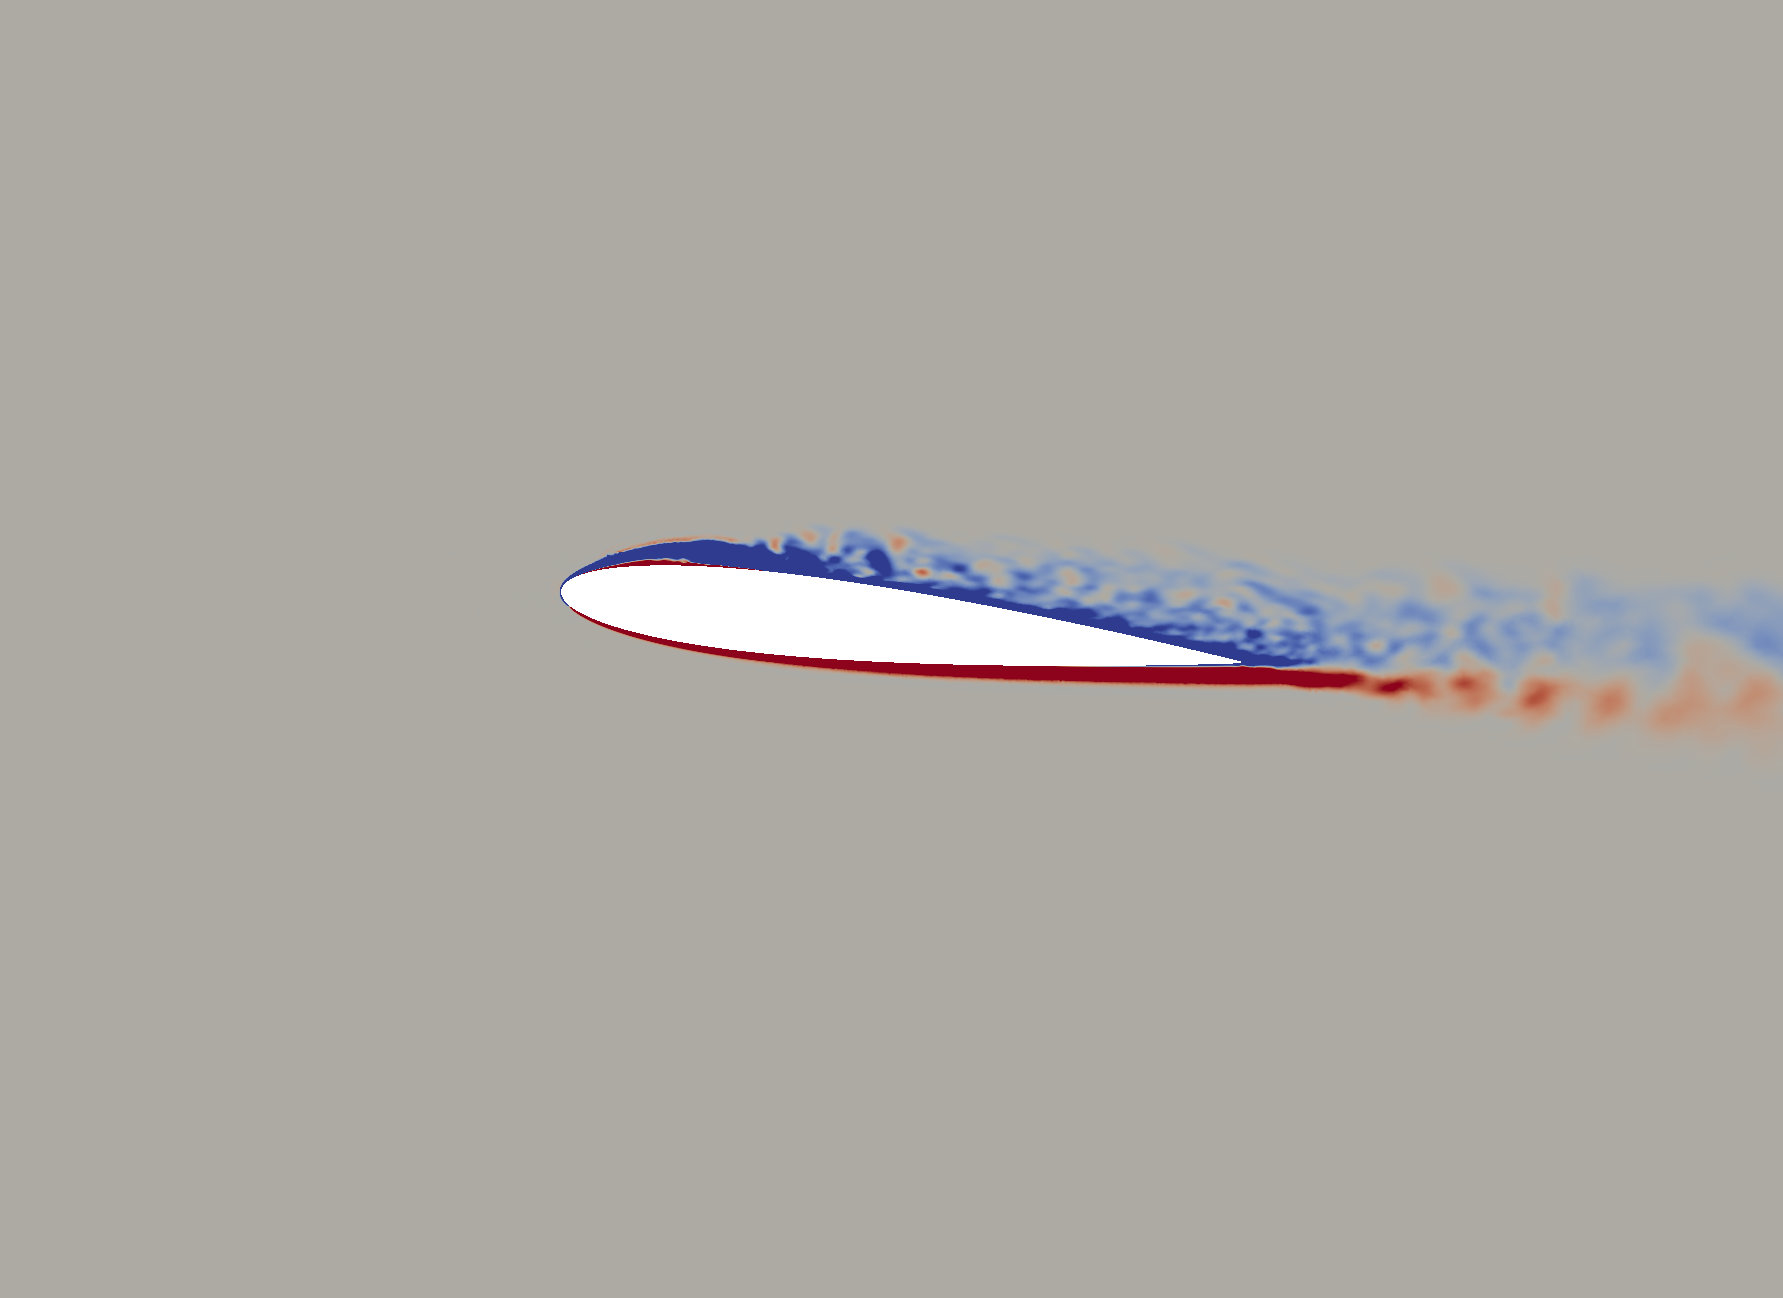
\includegraphics[width=1\textwidth]{figures/Vorticity_plots/Re_40k_1pt0/phase_195.png}
		\caption{$Re=4e4$, $\psi$ = $195^\circ$, $\tilde{t}=0.542$}
		\label{fig:Re_40k_1pt0_phi195}
	\end{subfigure}
	\begin{subfigure}[b]{0.32\textwidth}
		\centering
		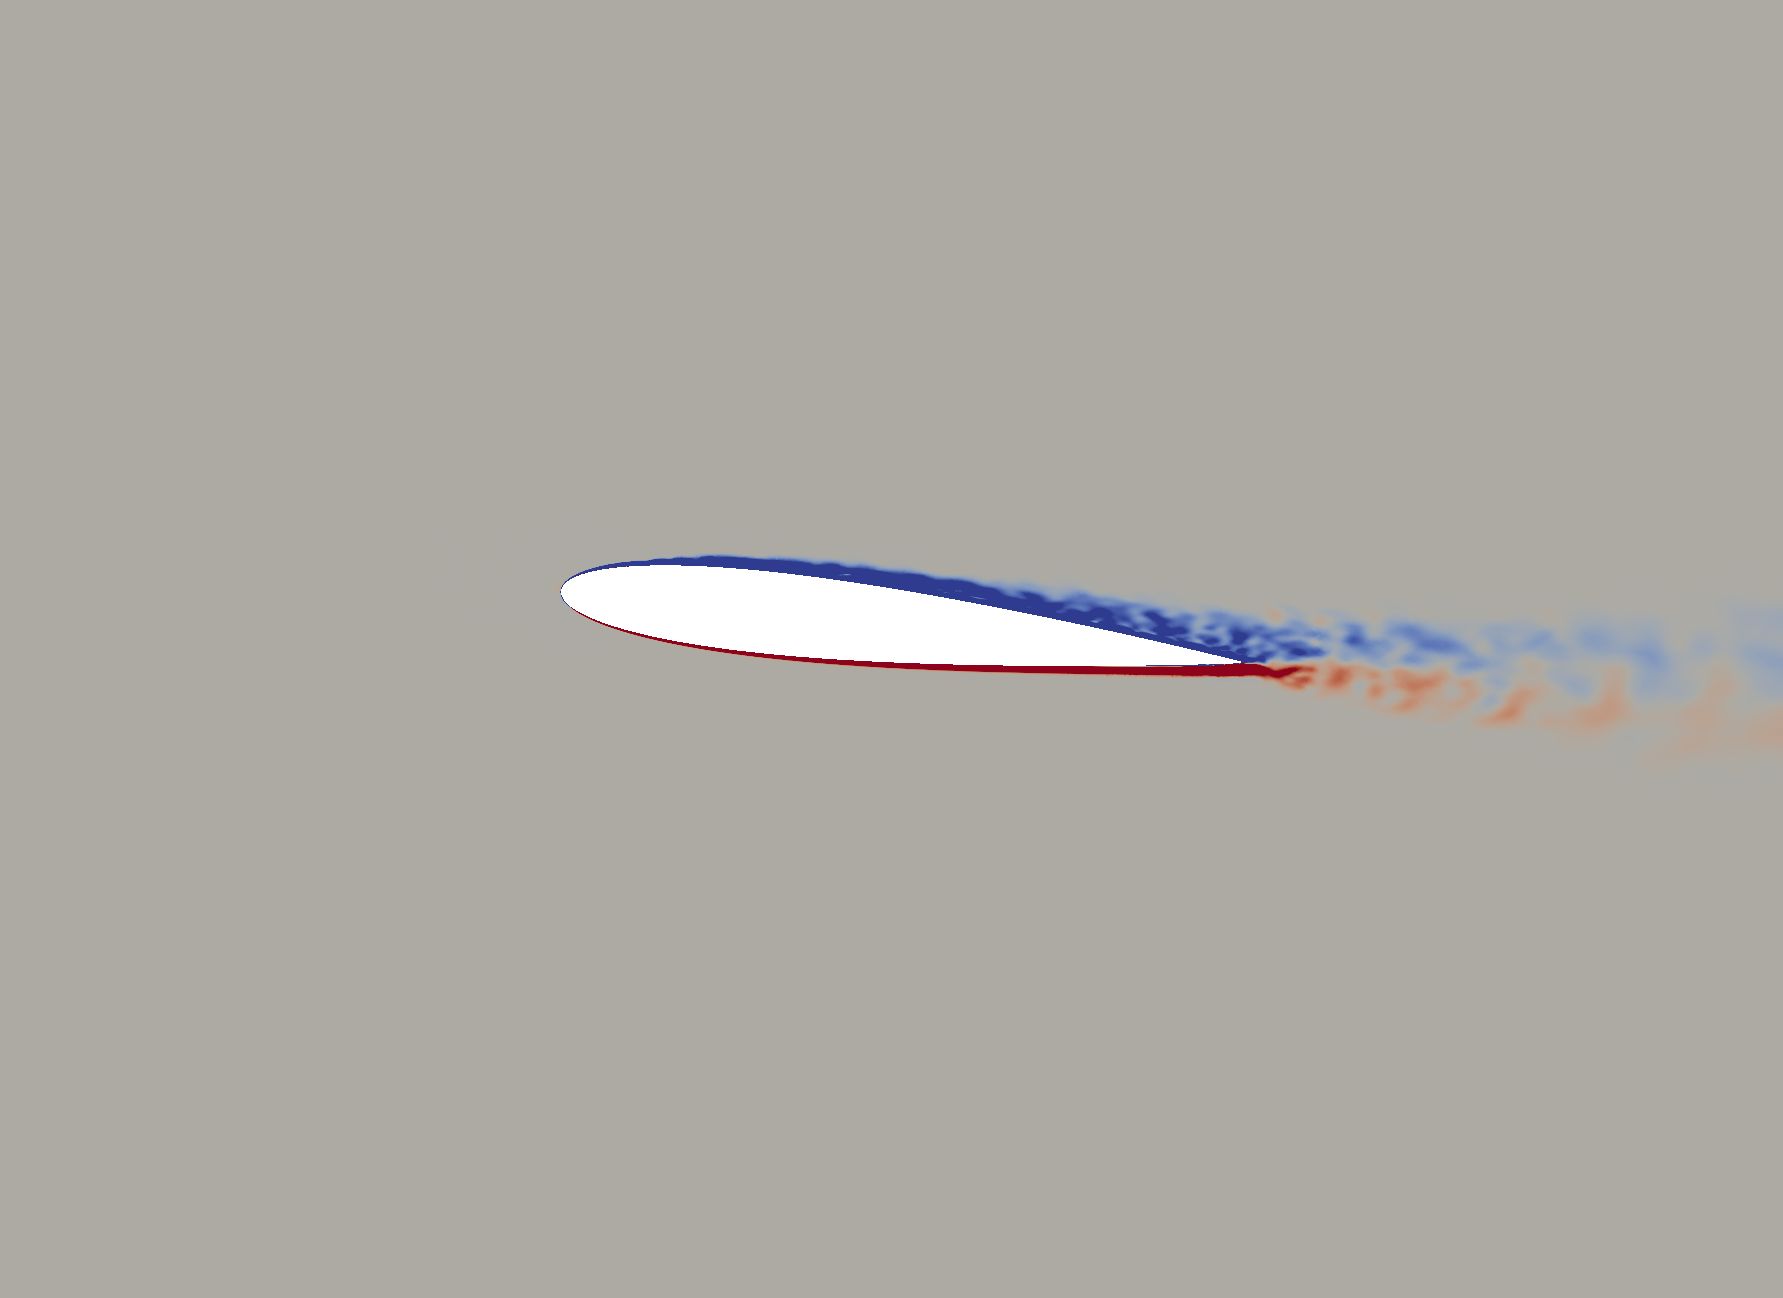
\includegraphics[width=1\textwidth]{figures/Vorticity_plots/Re_200k_1pt0/phase_195.png}
		\caption{$Re=2e5$, $\psi$ = $195^\circ$, $\tilde{t}=0.542$}
		\label{fig:Re_200k_1pt0_phi195}
	\end{subfigure}
	\begin{subfigure}[b]{0.32\textwidth}
		\centering
		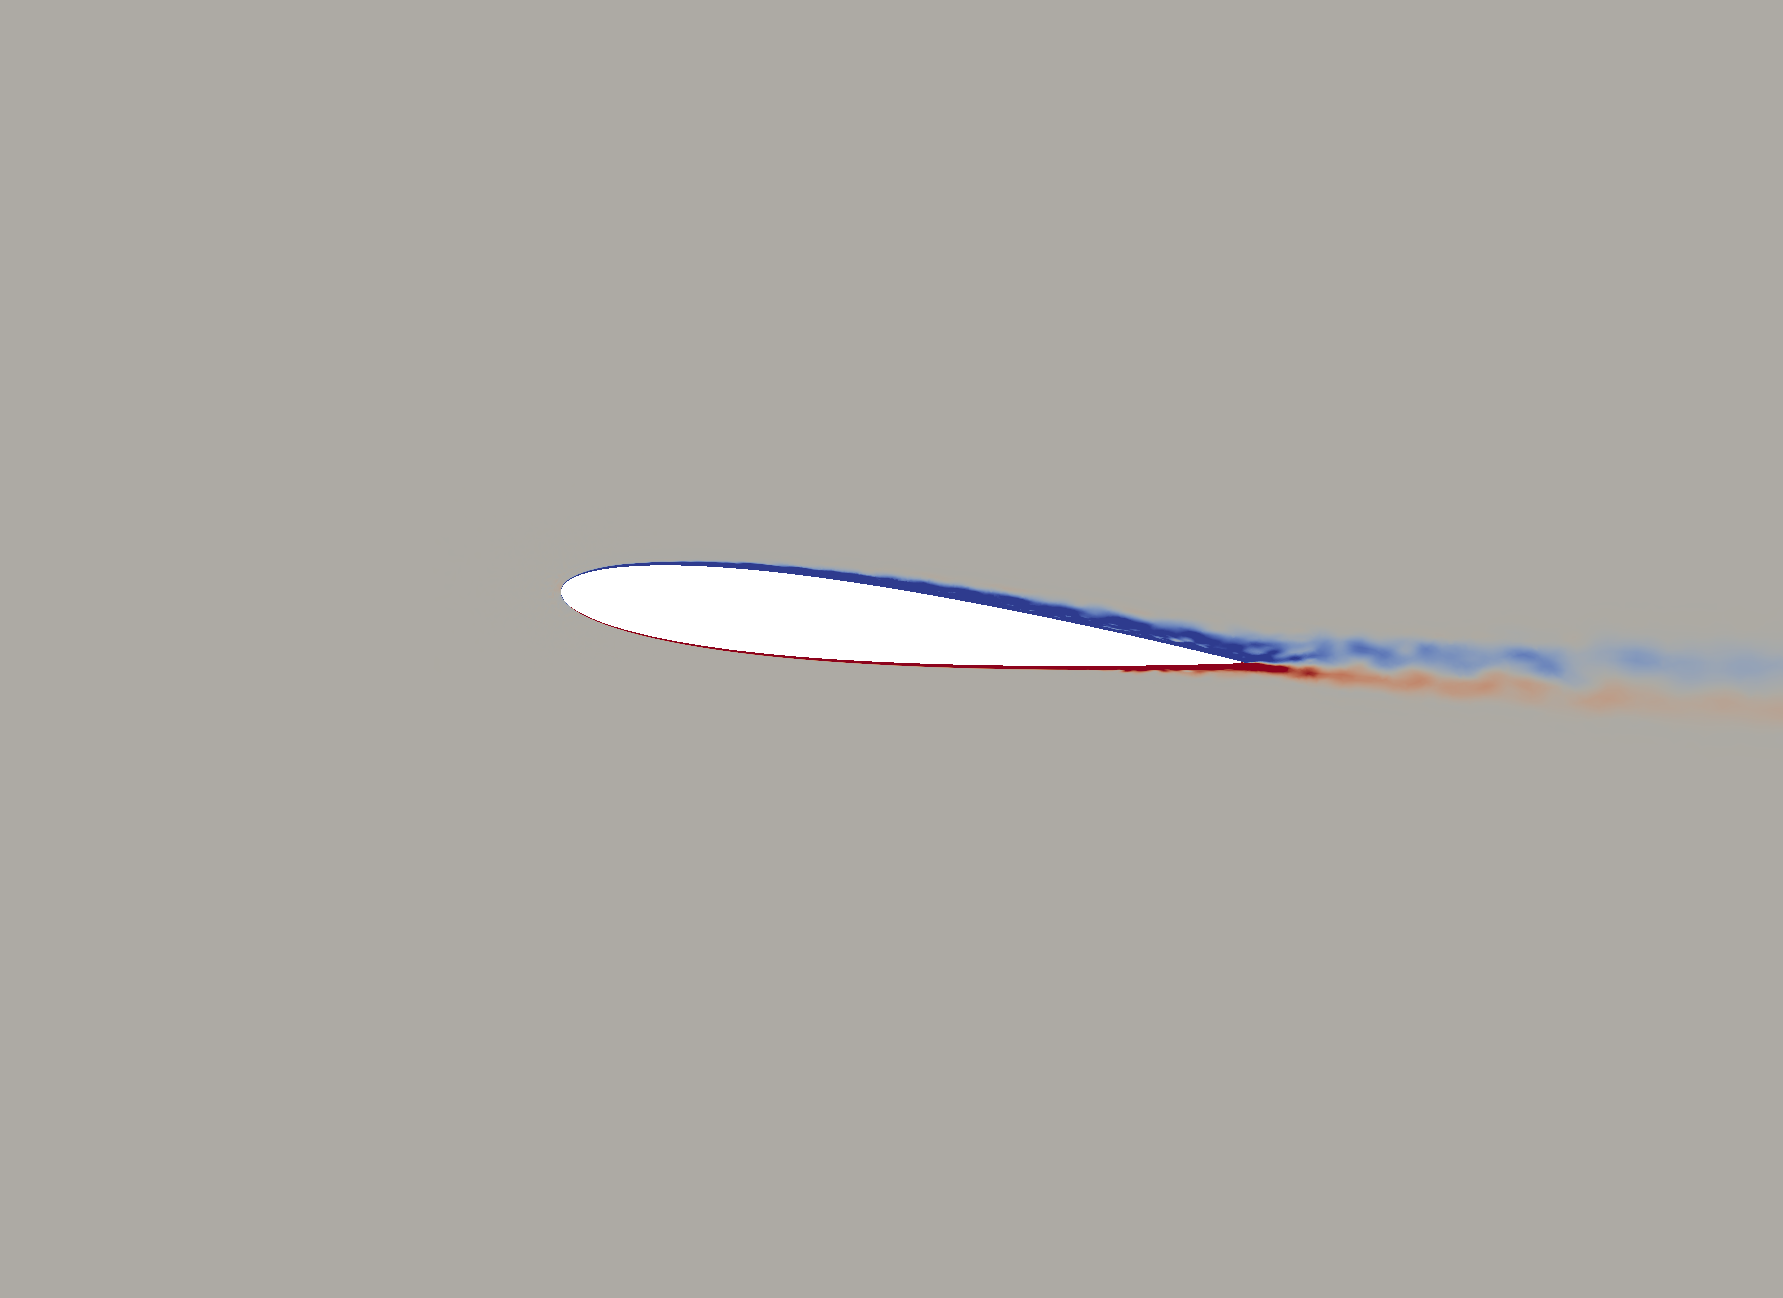
\includegraphics[width=1\textwidth]{figures/Vorticity_plots/Re_1m_1pt0/phase_195.png}
		\caption{$Re= 1e6$, $\psi$ = $195^\circ$, $\tilde{t}=0.542$}
		\label{fig:Re_1m_1pt0_phi195}
	\end{subfigure}
	
	\begin{subfigure}[b]{0.32\textwidth}
		\centering
		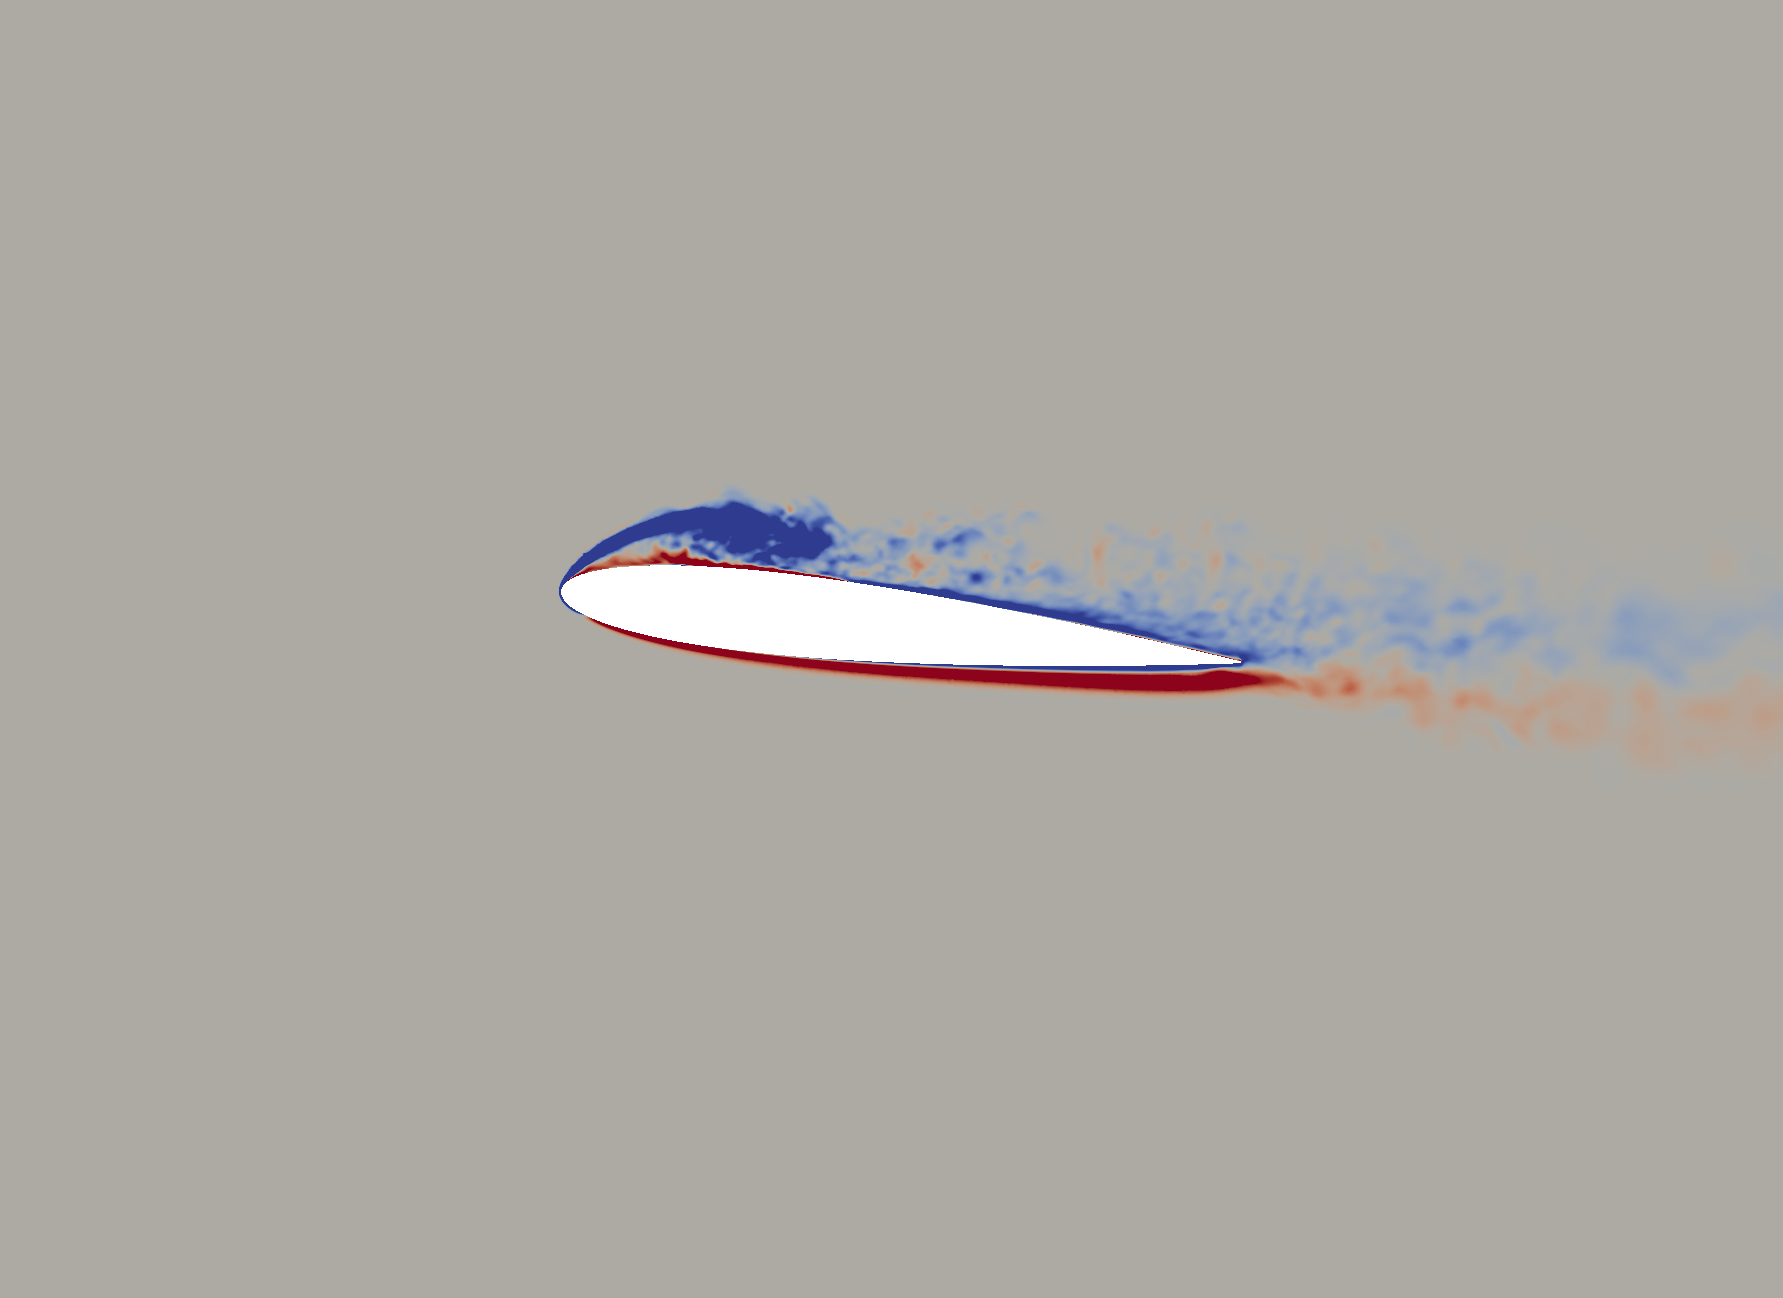
\includegraphics[width=1\textwidth]{figures/Vorticity_plots/Re_40k_1pt0/phase_225.png}
		\caption{$Re=4e4$, $\psi$ = $225^\circ$, $\tilde{t}=0.625$}
		\label{fig:Re_40k_1pt0_phi225}
	\end{subfigure}
	\begin{subfigure}[b]{0.32\textwidth}
		\centering
		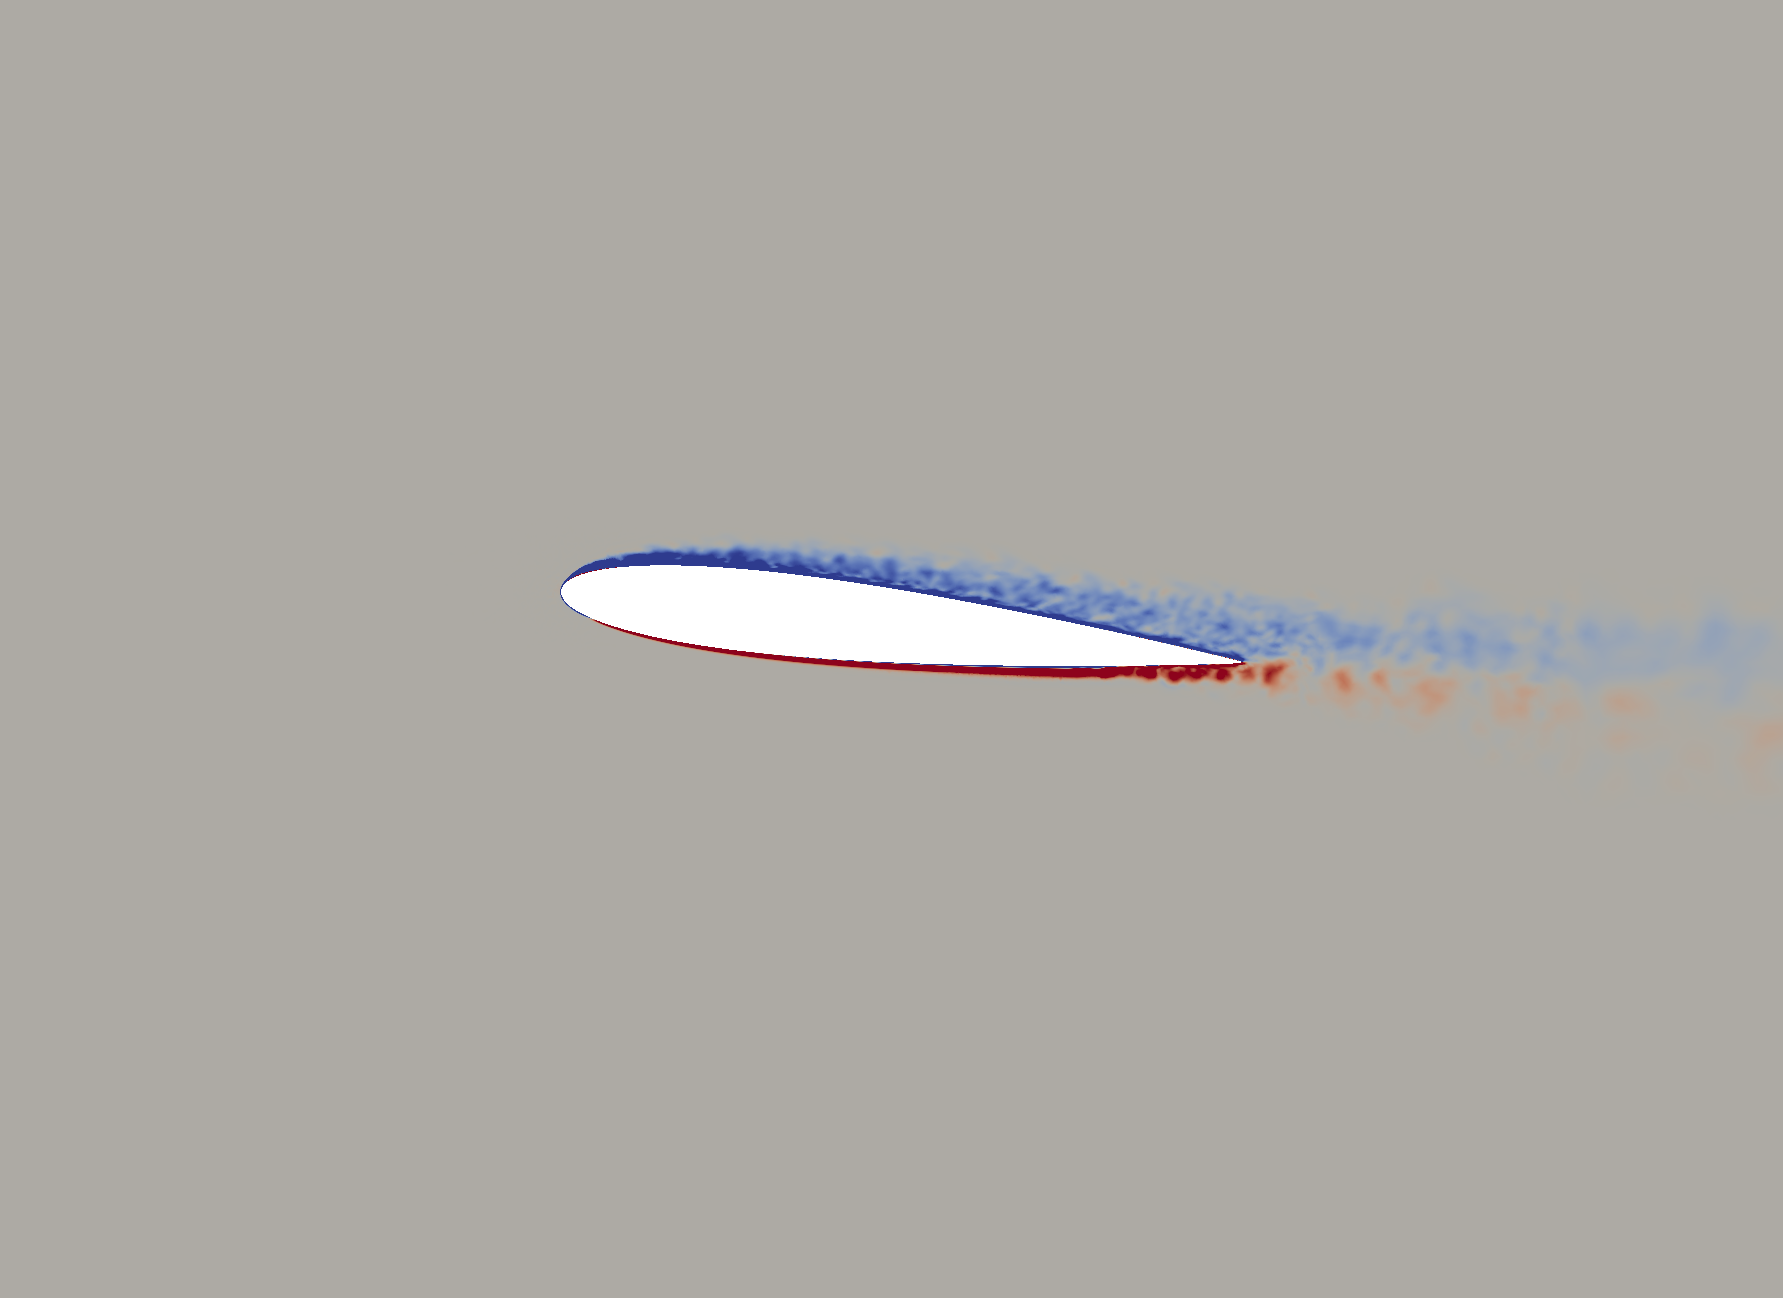
\includegraphics[width=1\textwidth]{figures/Vorticity_plots/Re_200k_1pt0/phase_225.png}
		\caption{$Re=2e5$, $\psi$ = $225^\circ$,  $\tilde{t}=0.625$}
		\label{fig:Re_200k_1pt0_phi225}
	\end{subfigure}
	\begin{subfigure}[b]{0.32\textwidth}
		\centering
		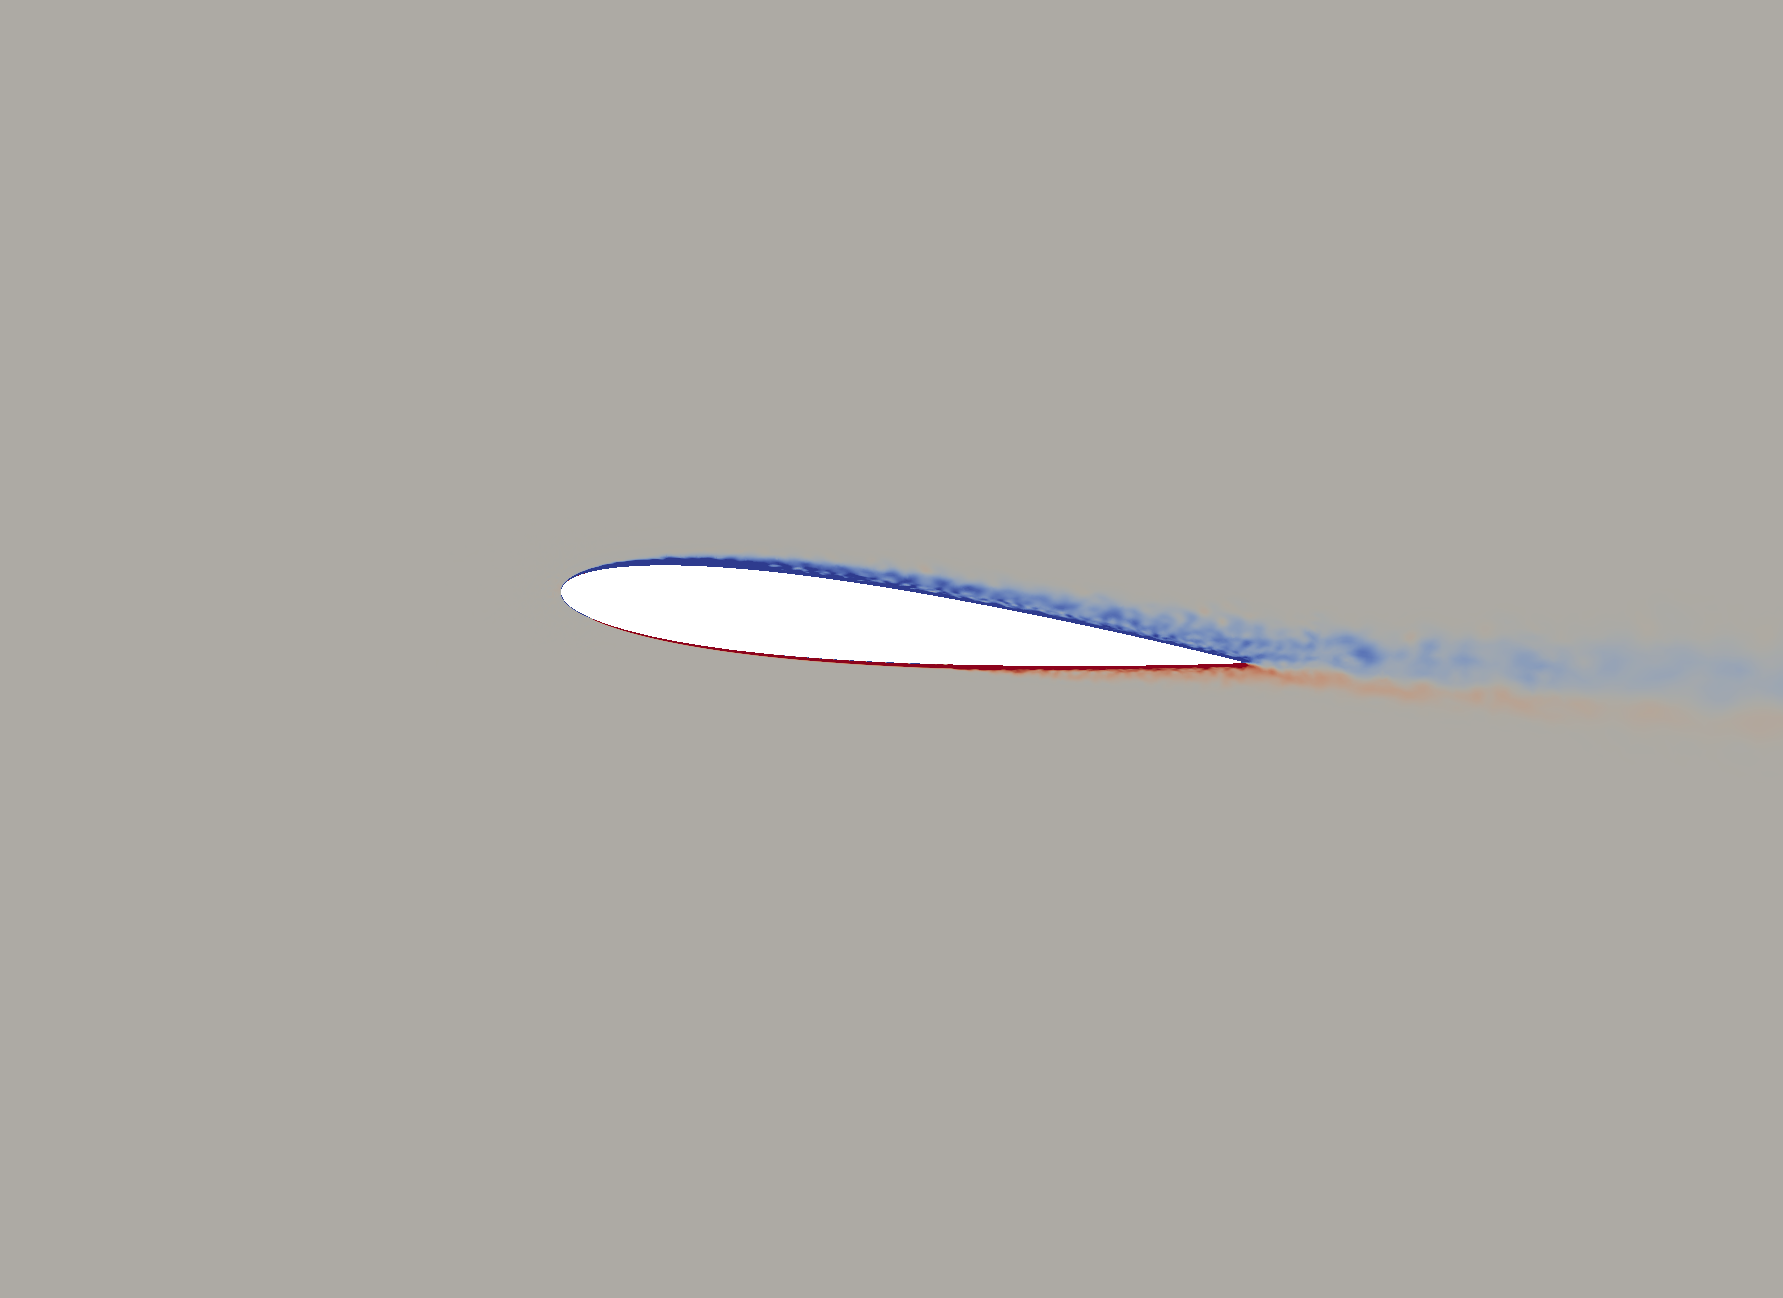
\includegraphics[width=1\textwidth]{figures/Vorticity_plots/Re_1m_1pt0/phase_225.png}
		\caption{$Re=1e6$, $\psi$ = $225^\circ$,  $\tilde{t}=0.625$}
		\label{fig:Re_1m_1pt0_phi225}
	\end{subfigure}
	
	\begin{subfigure}[b]{0.32\textwidth}
		\centering
		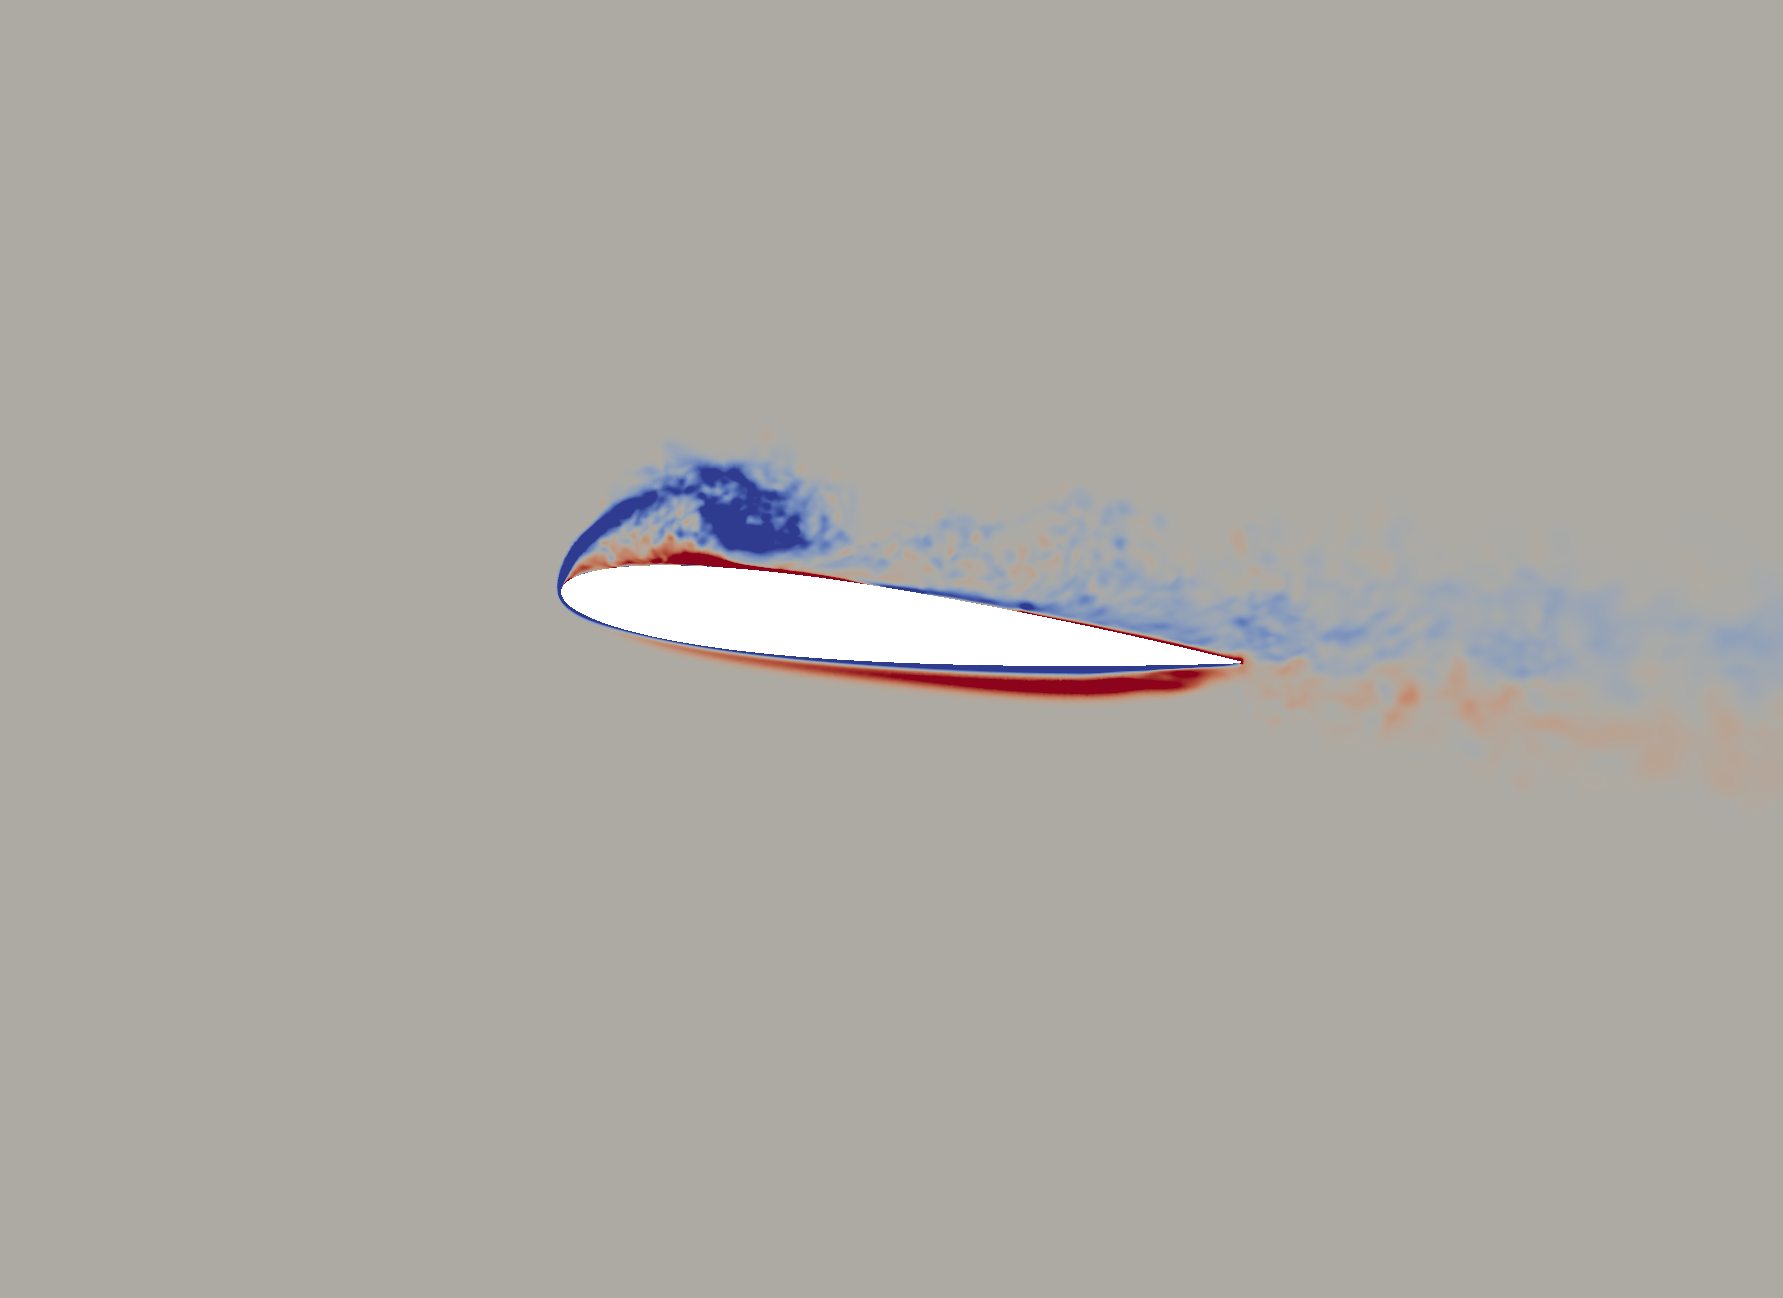
\includegraphics[width=1\textwidth]{figures/Vorticity_plots/Re_40k_1pt0/phase_240.png}
		\caption{$Re=4e4$, $\psi$ = $240^\circ$, $\tilde{t}=0.667$}
		\label{fig:Re_40k_1pt0_phi240}
	\end{subfigure}
	\begin{subfigure}[b]{0.32\textwidth}
		\centering
		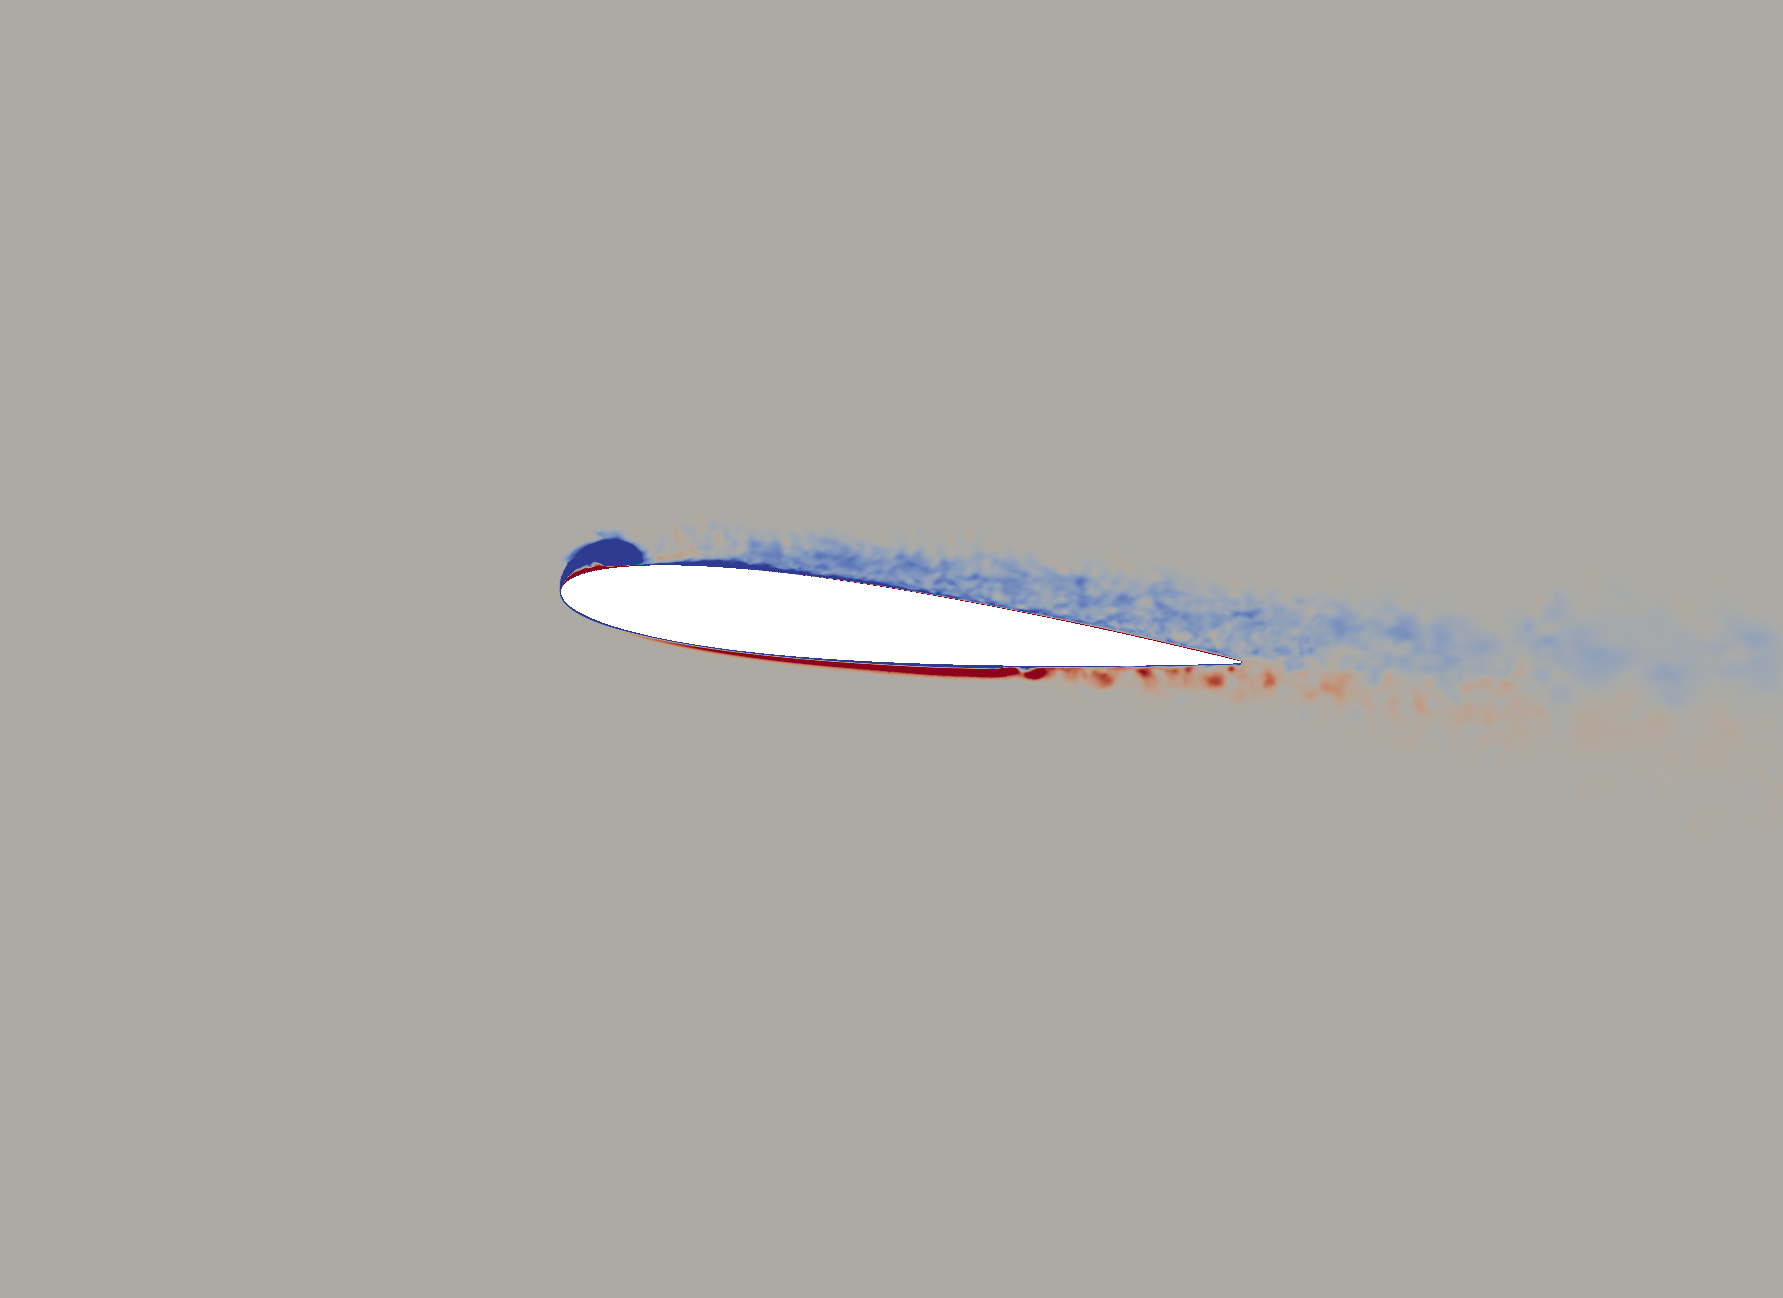
\includegraphics[width=1\textwidth]{figures/Vorticity_plots/Re_200k_1pt0/phase_240.png}
		\caption{$Re=2e5$, $\psi$ = $240^\circ$, $\tilde{t}=0.667$}
		\label{fig:Re_200k_1pt0_phi240}
	\end{subfigure}
	\begin{subfigure}[b]{0.32\textwidth}
		\centering
		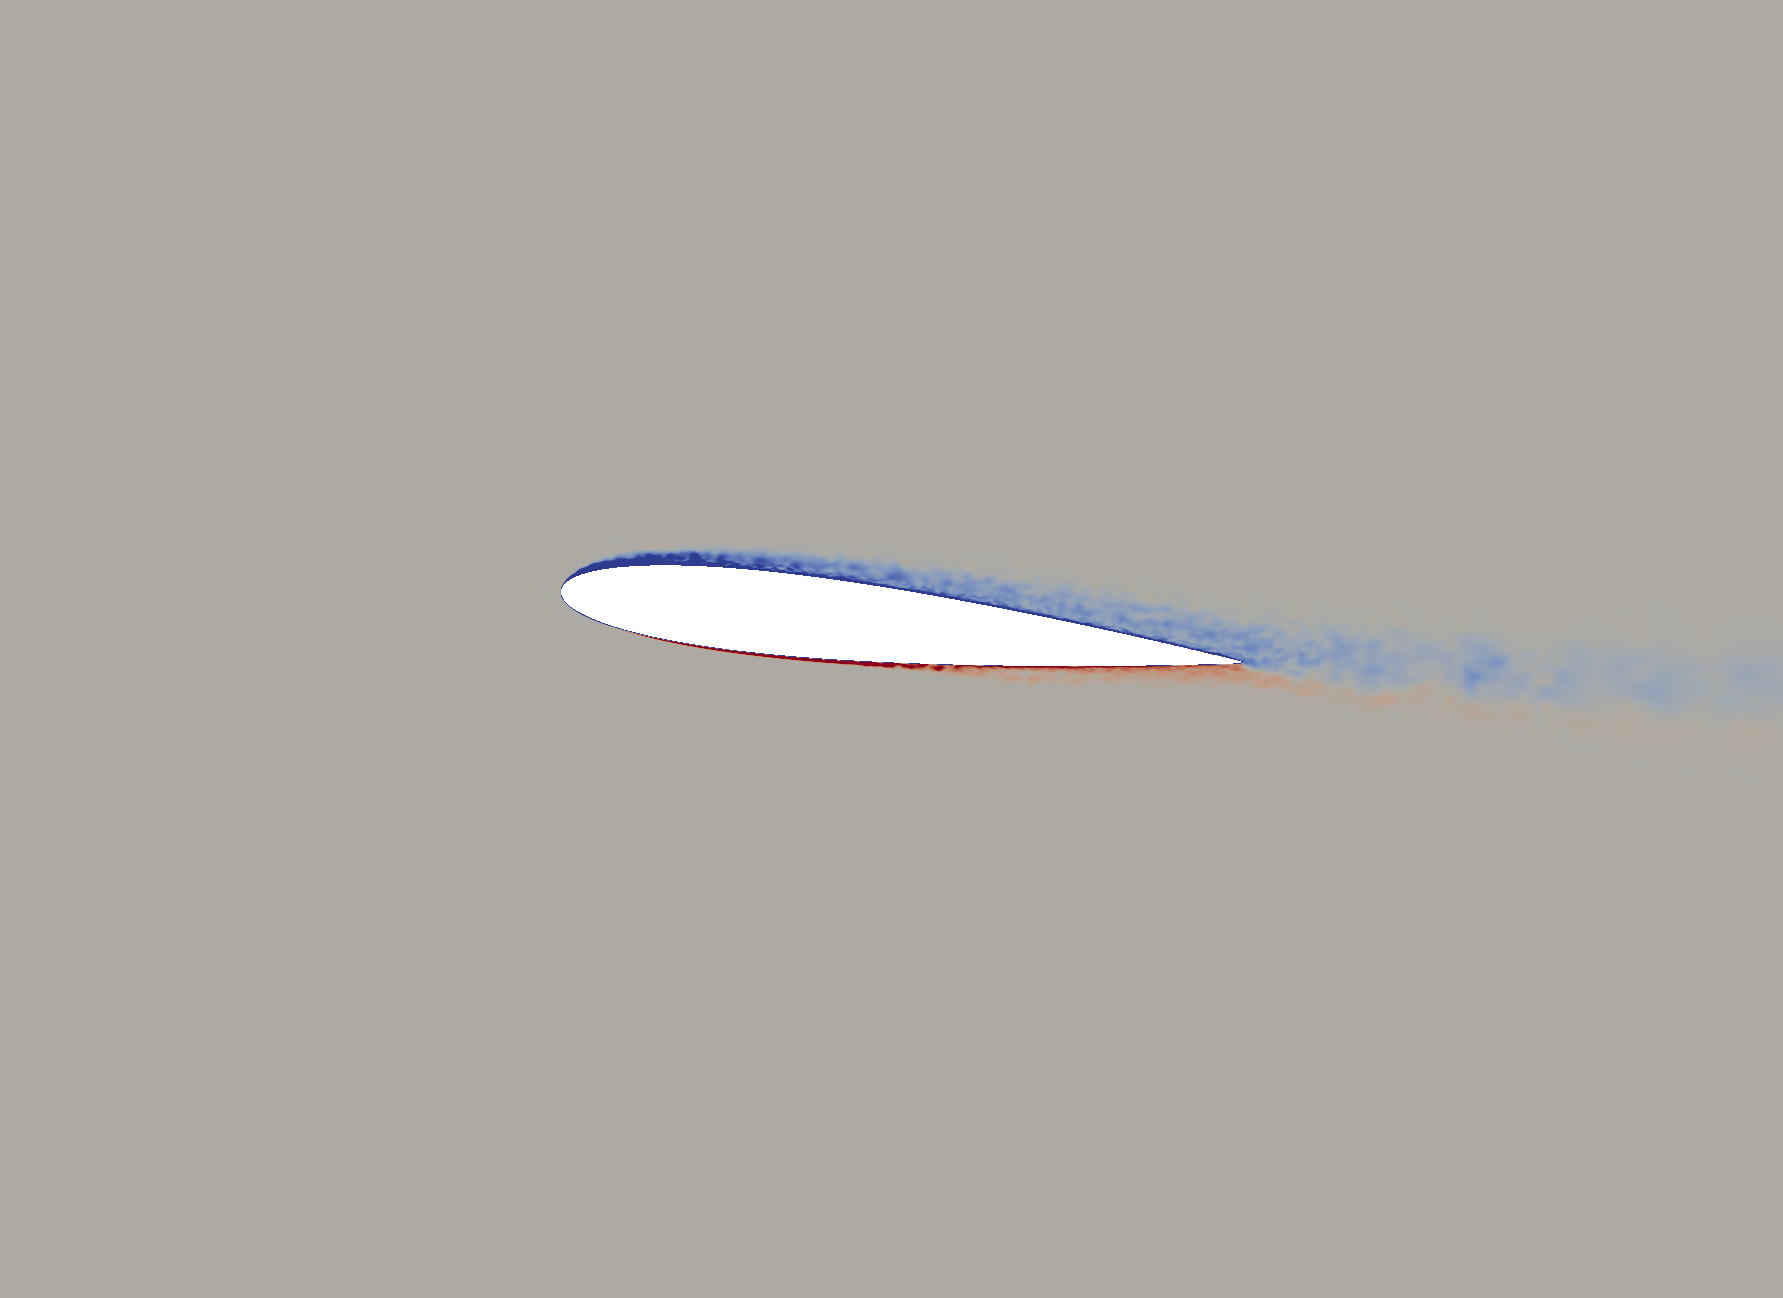
\includegraphics[width=1\textwidth]{figures/Vorticity_plots/Re_1m_1pt0/phase_240.png}
		\caption{$Re=1e6$, $\psi$ = $240^\circ$, $\tilde{t}=0.667$}
		\label{fig:Re_1m_1pt0_phi240}
	\end{subfigure}
	
	\begin{subfigure}[b]{0.32\textwidth}
		\centering
		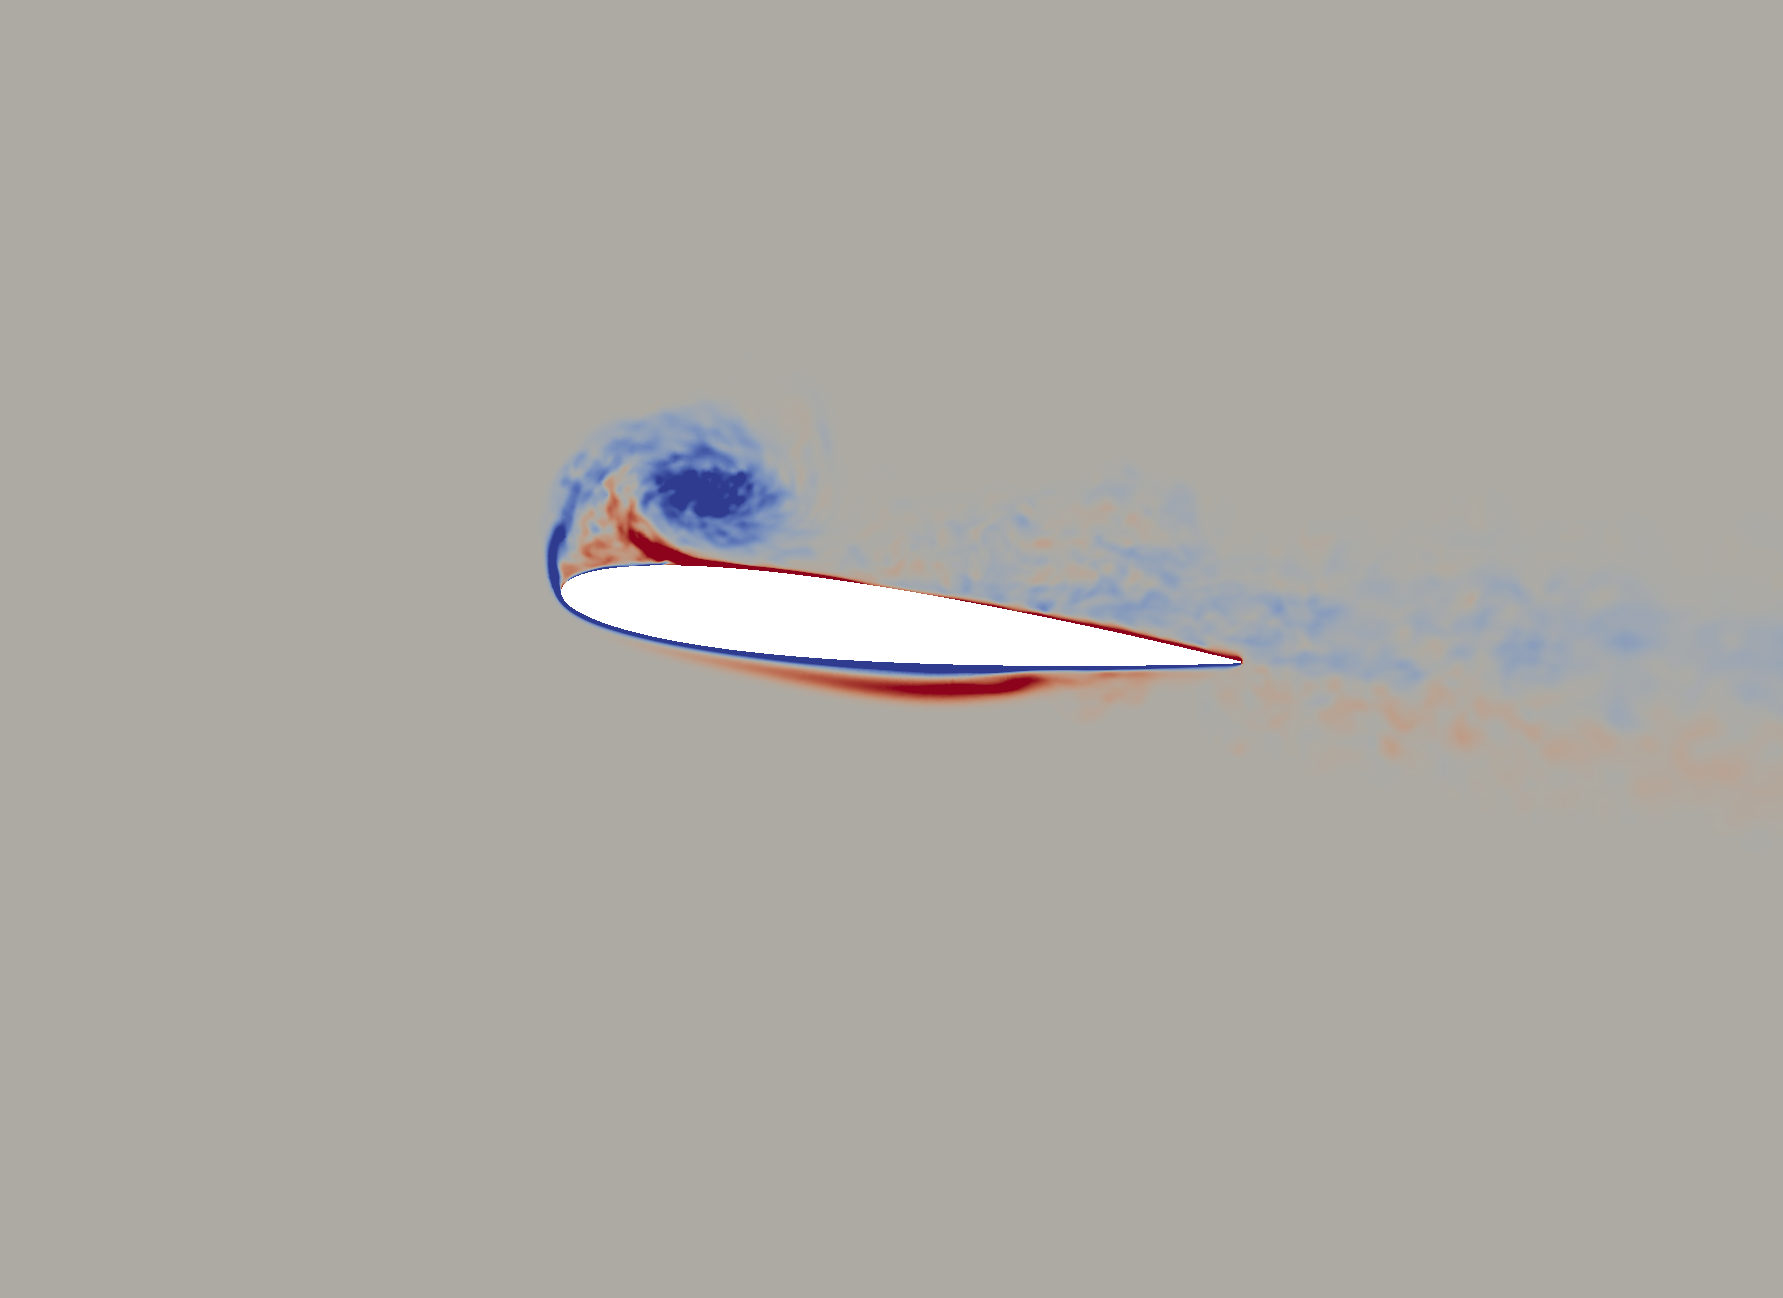
\includegraphics[width=1\textwidth]{figures/Vorticity_plots/Re_40k_1pt0/phase_255.png}
		\caption{$Re=4e4$, $\psi$ = $255^\circ$, $\tilde{t}=0.708$}
		\label{fig:Re_40k_1pt0_phi255}
	\end{subfigure}
	\begin{subfigure}[b]{0.32\textwidth}
		\centering
		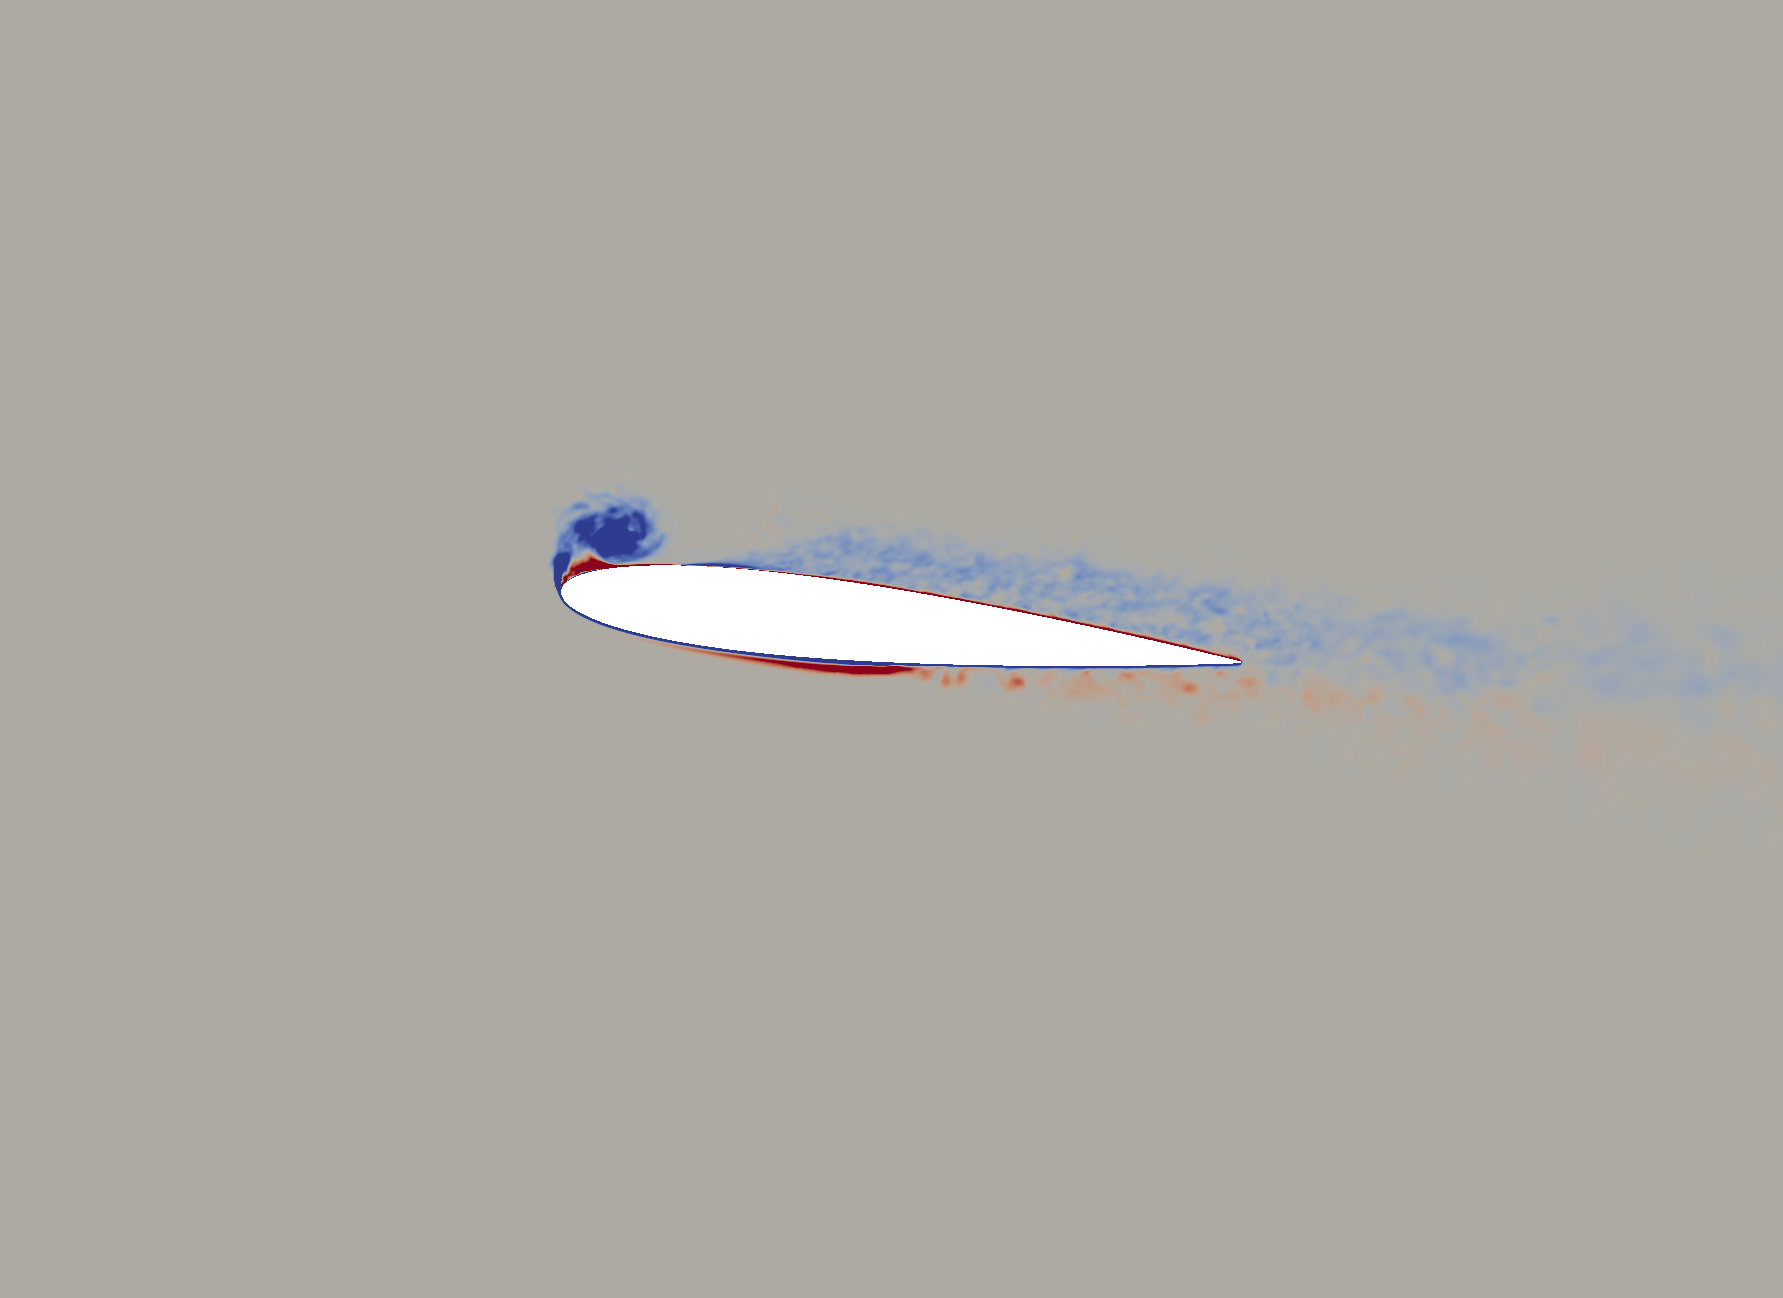
\includegraphics[width=1\textwidth]{figures/Vorticity_plots/Re_200k_1pt0/phase_255.png}
		\caption{$Re=2e5$, $\psi$ = $255^\circ$, $\tilde{t}=0.708$}
		\label{fig:Re_200k_1pt0_phi255}
	\end{subfigure}
	\begin{subfigure}[b]{0.32\textwidth}
		\centering
		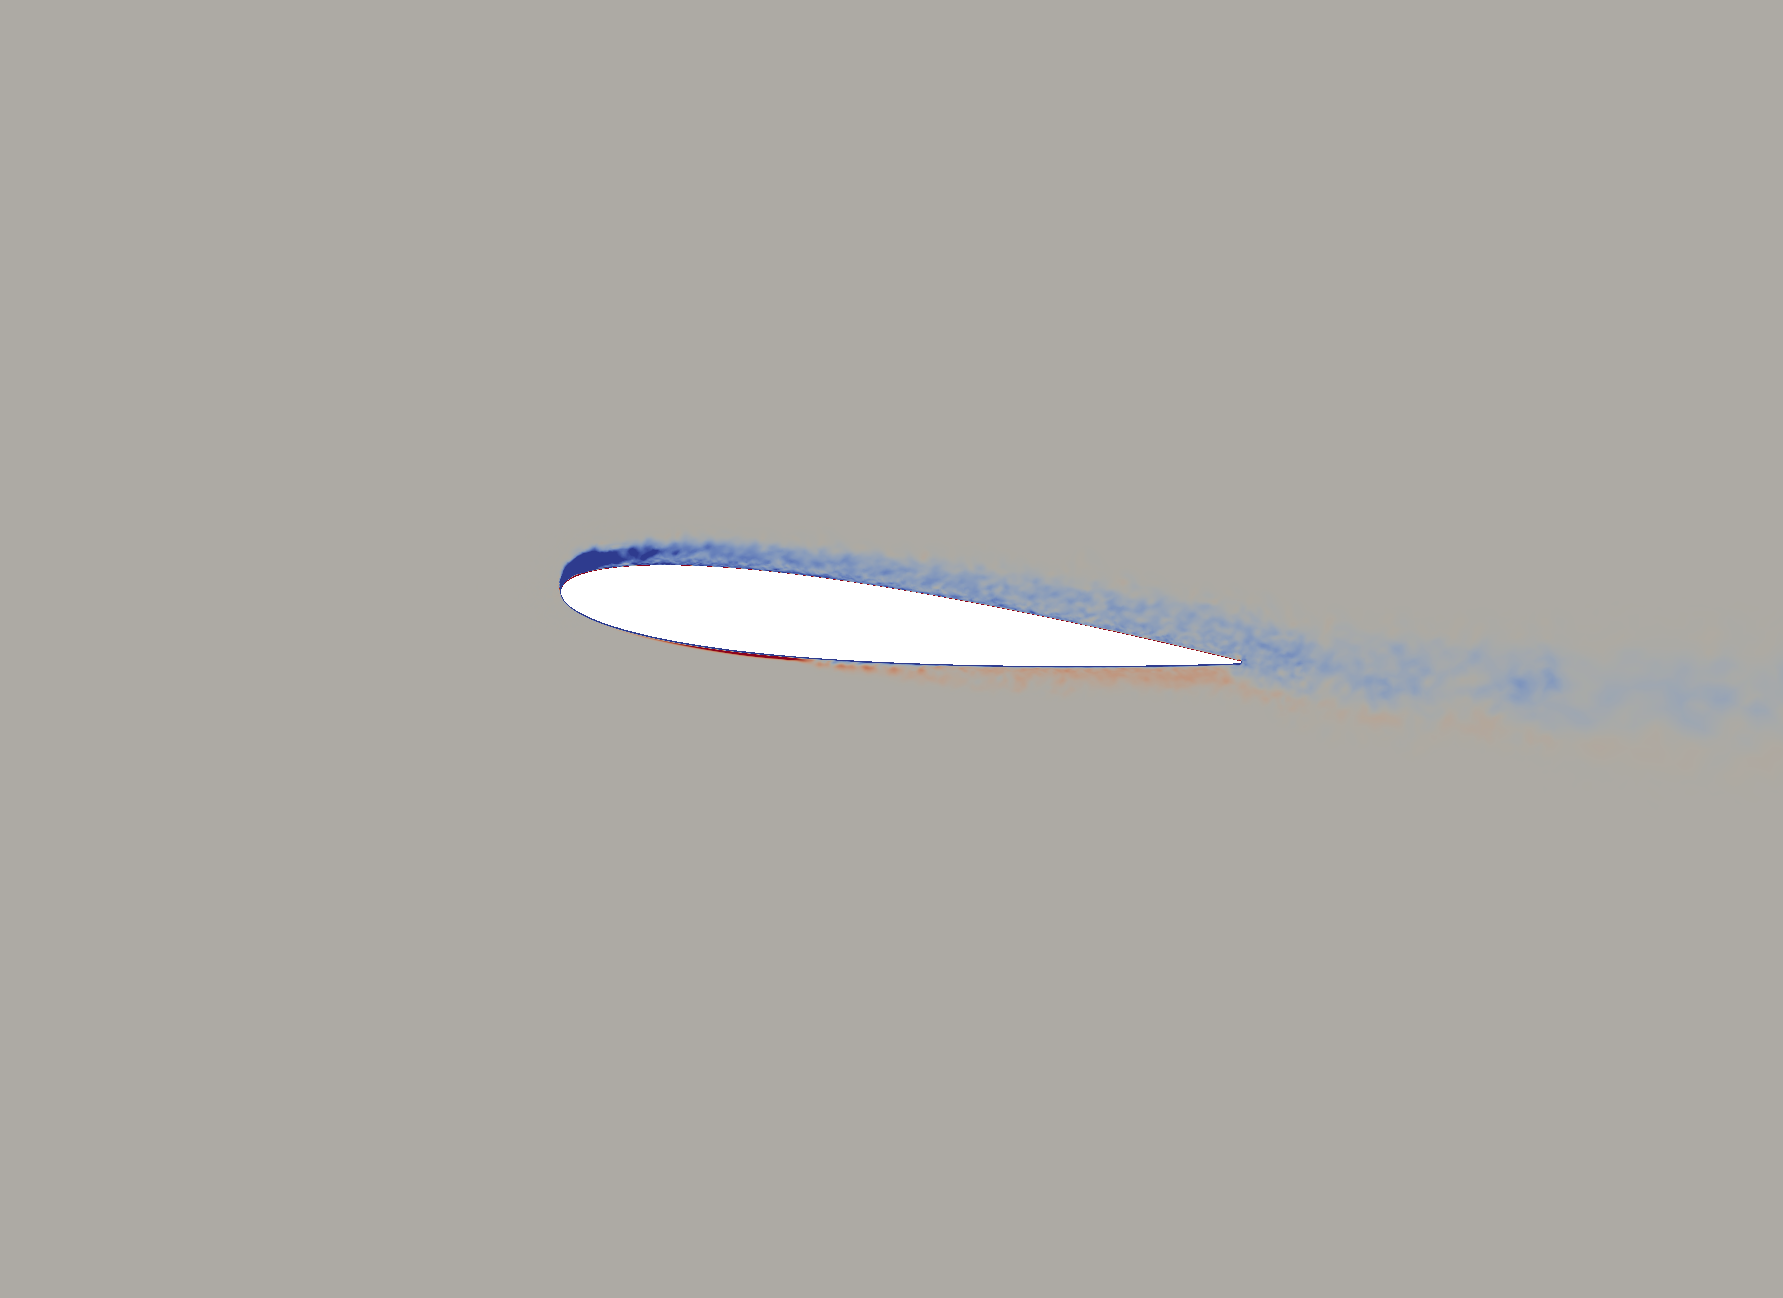
\includegraphics[width=1\textwidth]{figures/Vorticity_plots/Re_1m_1pt0/phase_255.png}
		\caption{$Re=1e6$, $\psi$ = $255^\circ$, $\tilde{t}=0.708$}
		\label{fig:Re_1m_1pt0_phi255}
	\end{subfigure}
	
	\caption{Spanwise vorticity at 8 different phases for $Re$=40,000 (left column), 200,000 (middle column) and 1,000,000 (right column) at $\lambda$ = 1.0}
	\label{fig:vortScreen_1pt0}
\end{figure}


\begin{figure}[H]\ContinuedFloat
	\centering
	\begin{subfigure}[b]{0.32\textwidth}
		\centering
		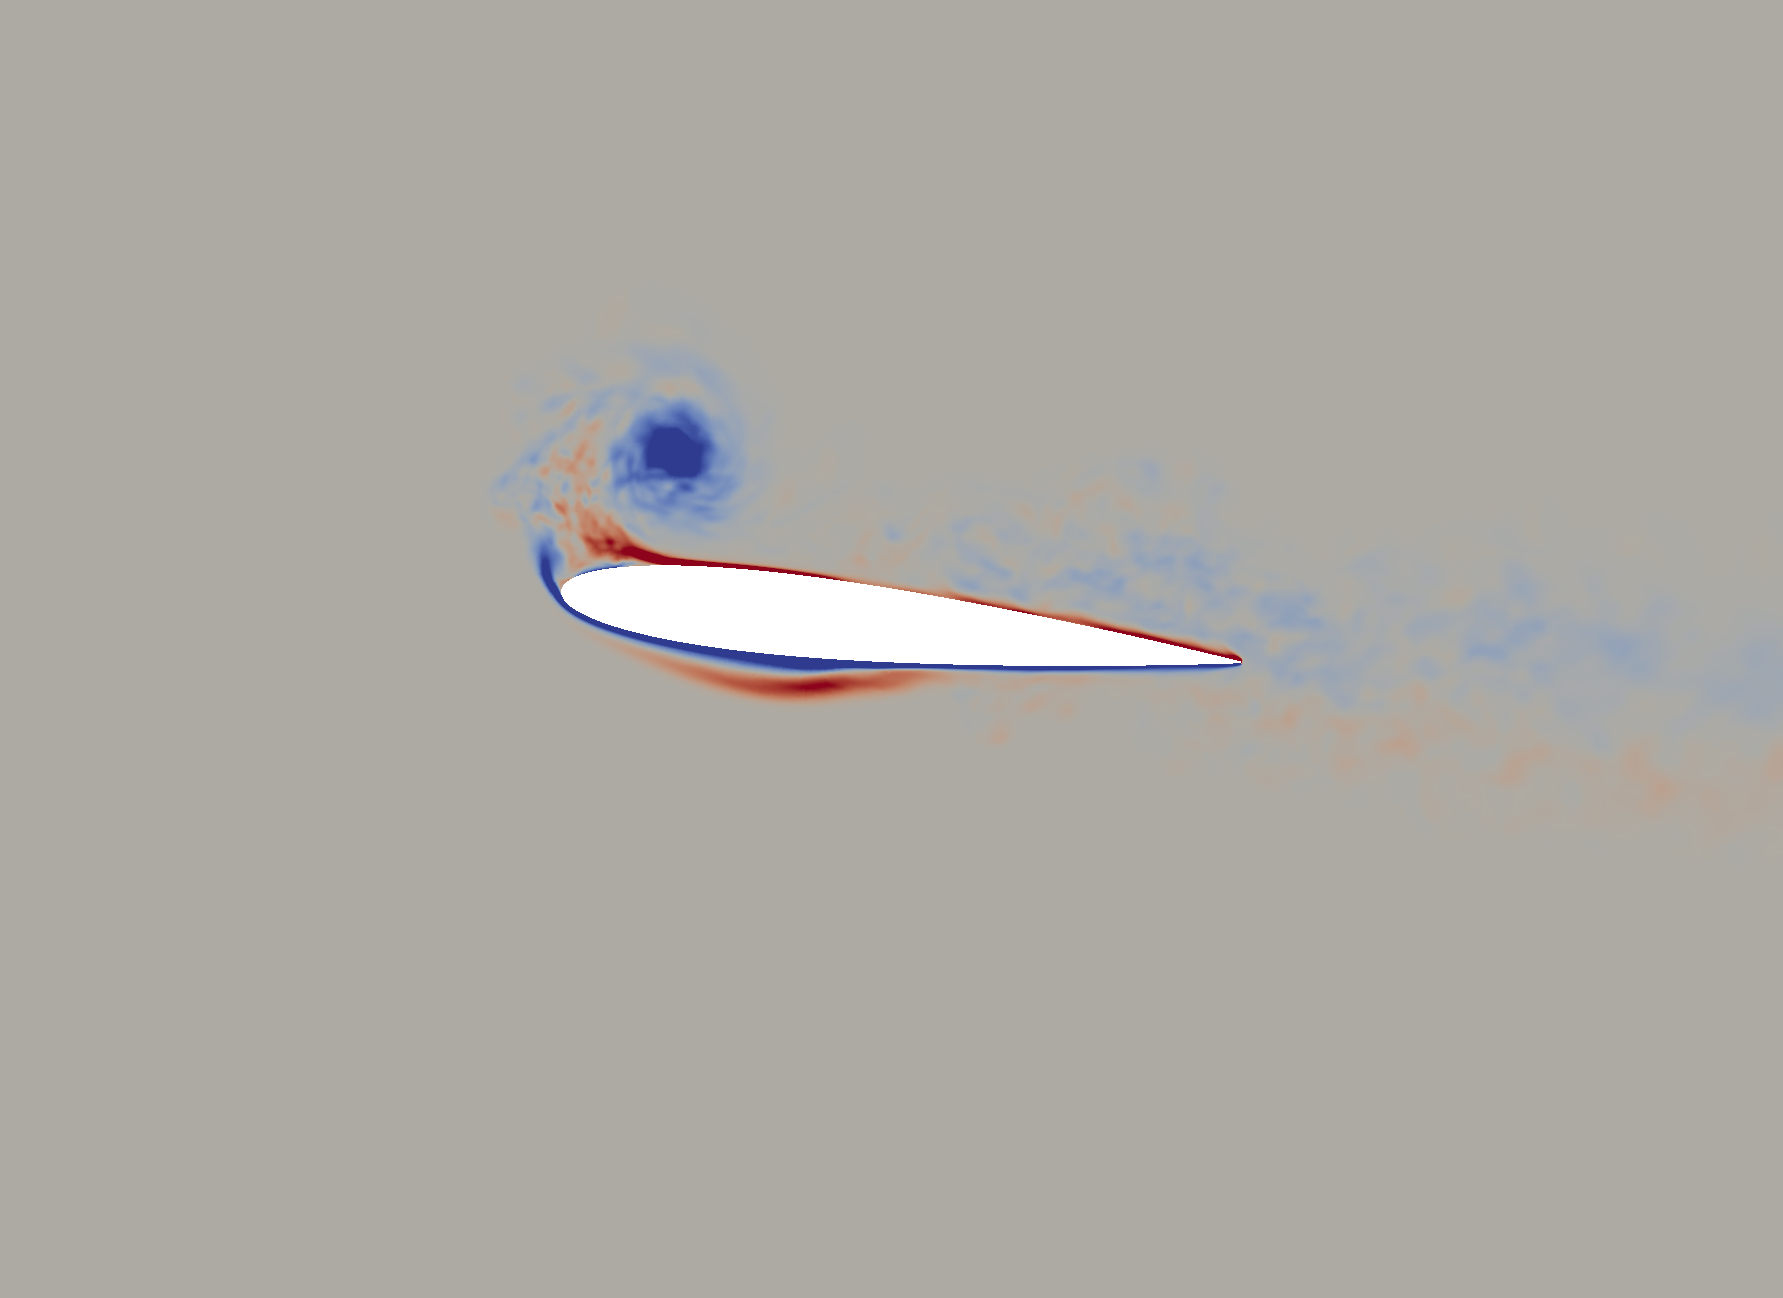
\includegraphics[width=1\textwidth]{figures/Vorticity_plots/Re_40k_1pt0/phase_270.png}
		\caption{$Re=4e4$, $\psi$ = $270^\circ$, $\tilde{t}=0.750$}
		\label{fig:Re_40k_1pt0_phi270}
	\end{subfigure}
	\begin{subfigure}[b]{0.32\textwidth}
		\centering
		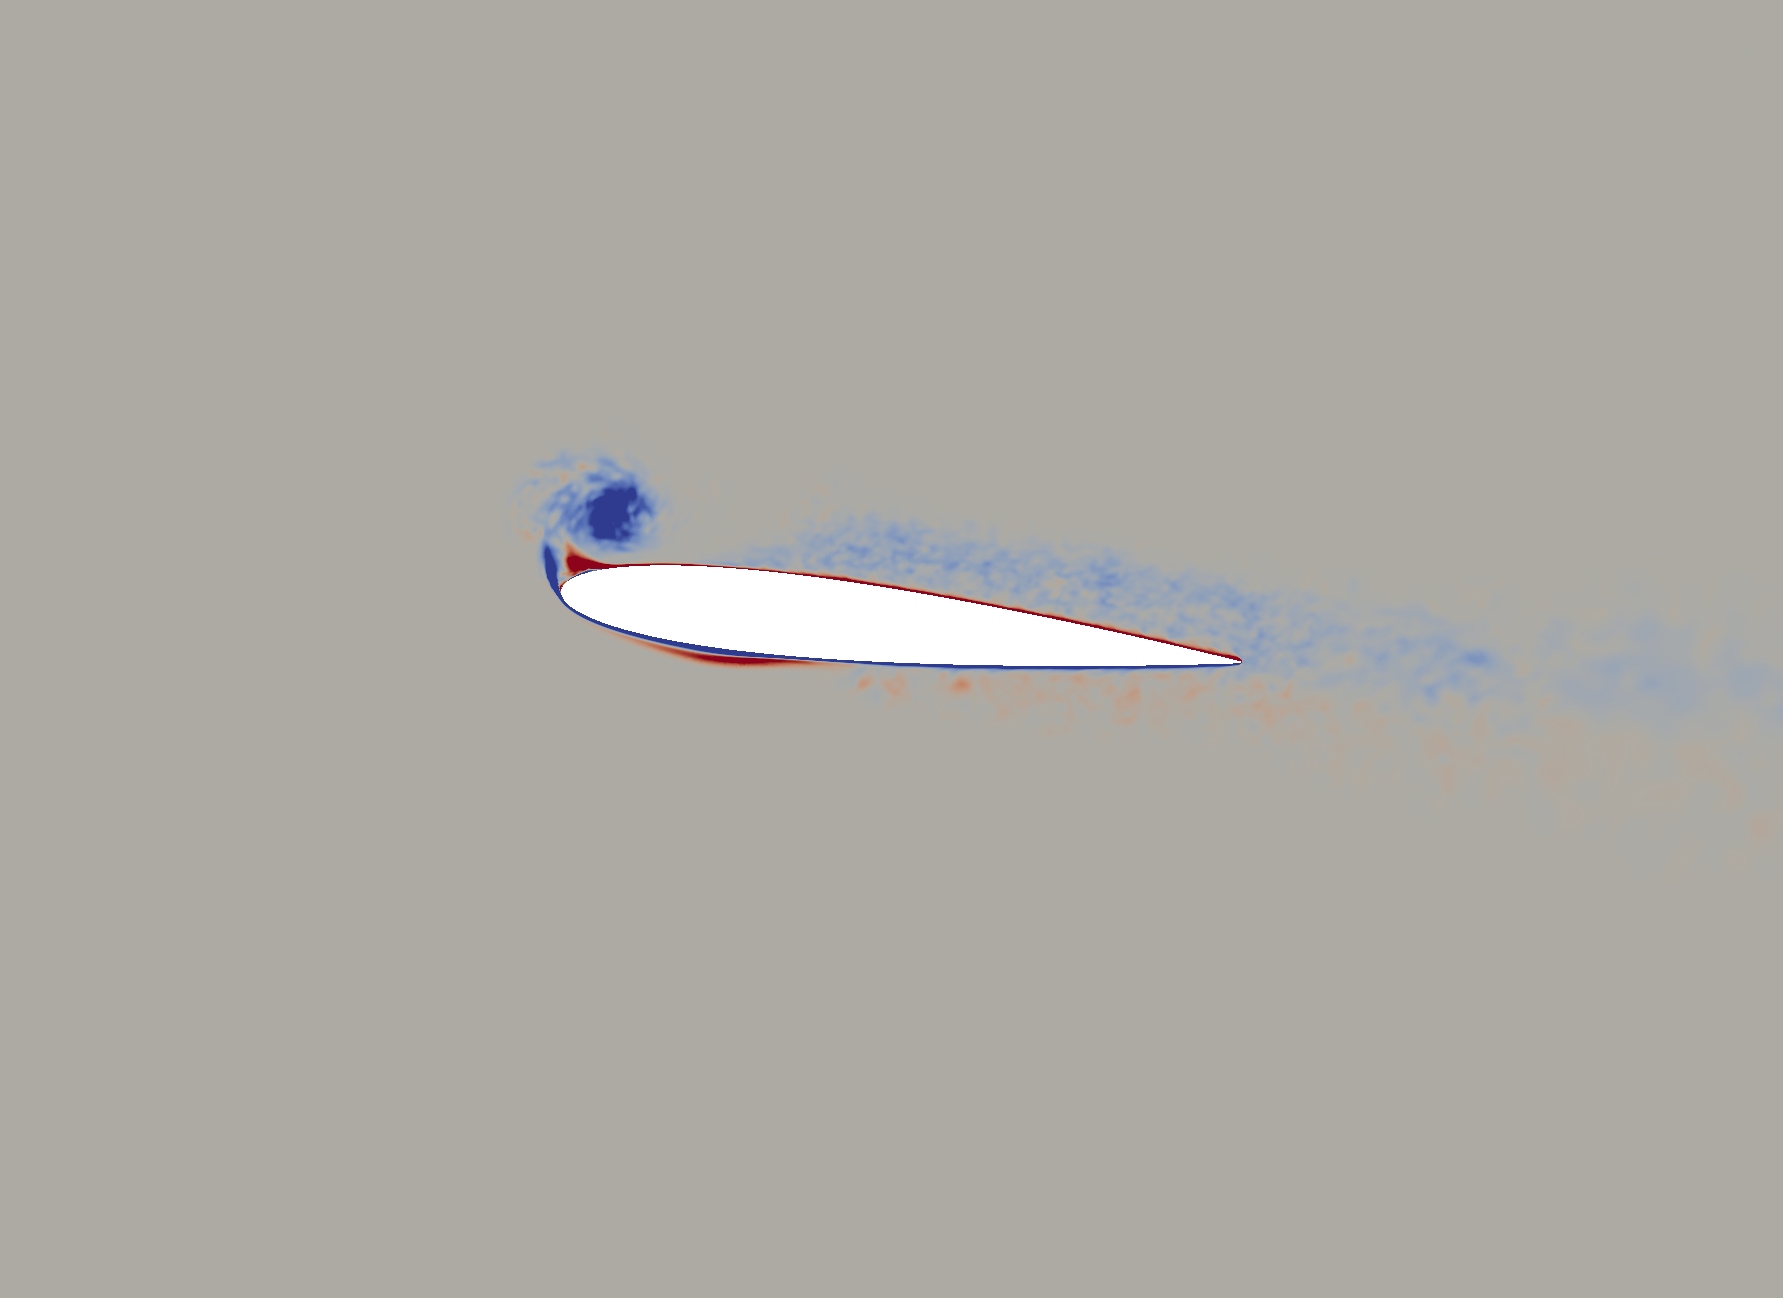
\includegraphics[width=1\textwidth]{figures/Vorticity_plots/Re_200k_1pt0/phase_270.png}
		\caption{$Re=2e5$, $\psi$ = $270^\circ$, $\tilde{t}=0.750$}
		\label{fig:Re_200k_1pt0_phi270}
	\end{subfigure}
	\begin{subfigure}[b]{0.32\textwidth}
		\centering
		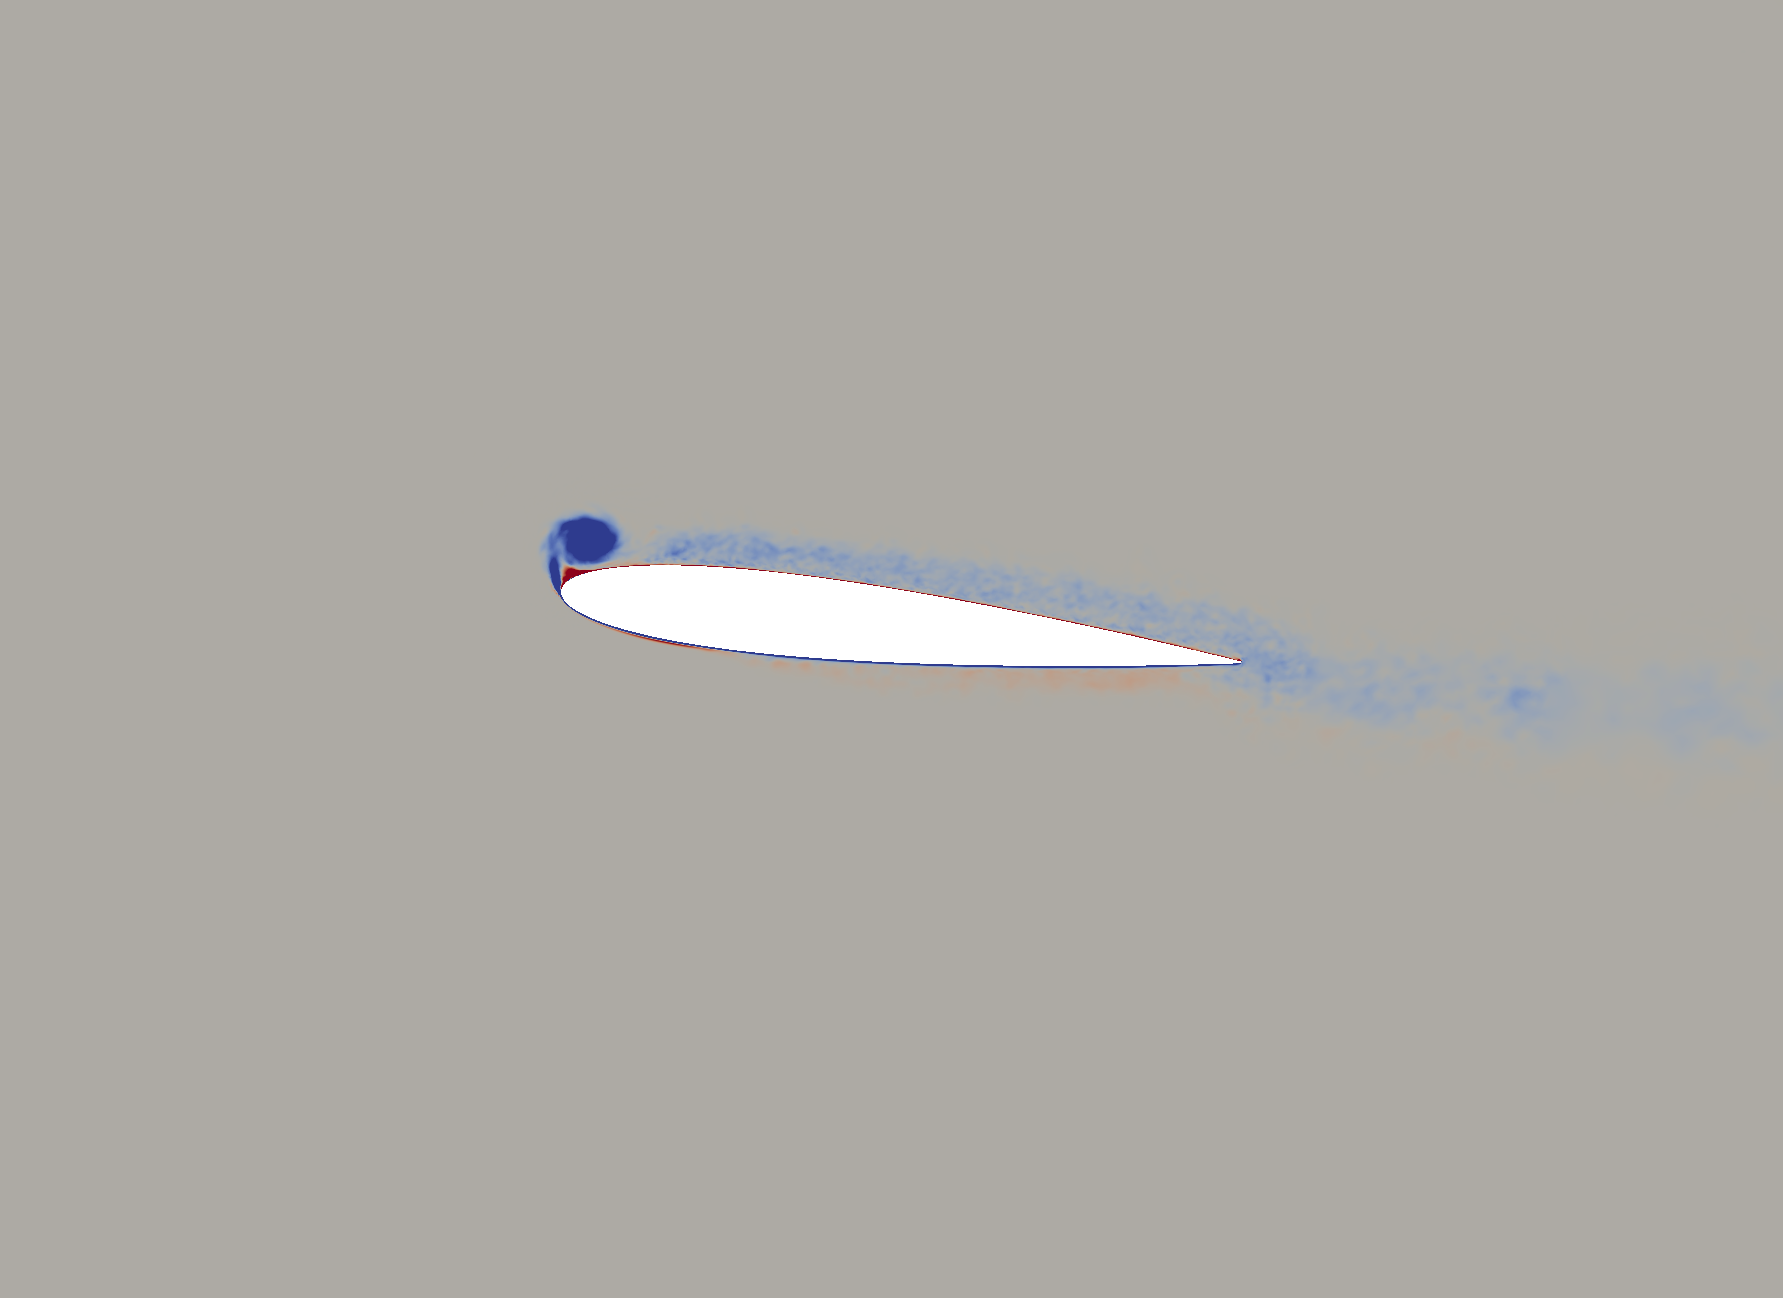
\includegraphics[width=1\textwidth]{figures/Vorticity_plots/Re_1m_1pt0/phase_270.png}
		\caption{$Re=1e6$, $\psi$ = $270^\circ$, $\tilde{t}=0.750$}
		\label{fig:Re_1m_1pt0_phi270}
	\end{subfigure}
	
	\begin{subfigure}[b]{0.32\textwidth}
		\centering
		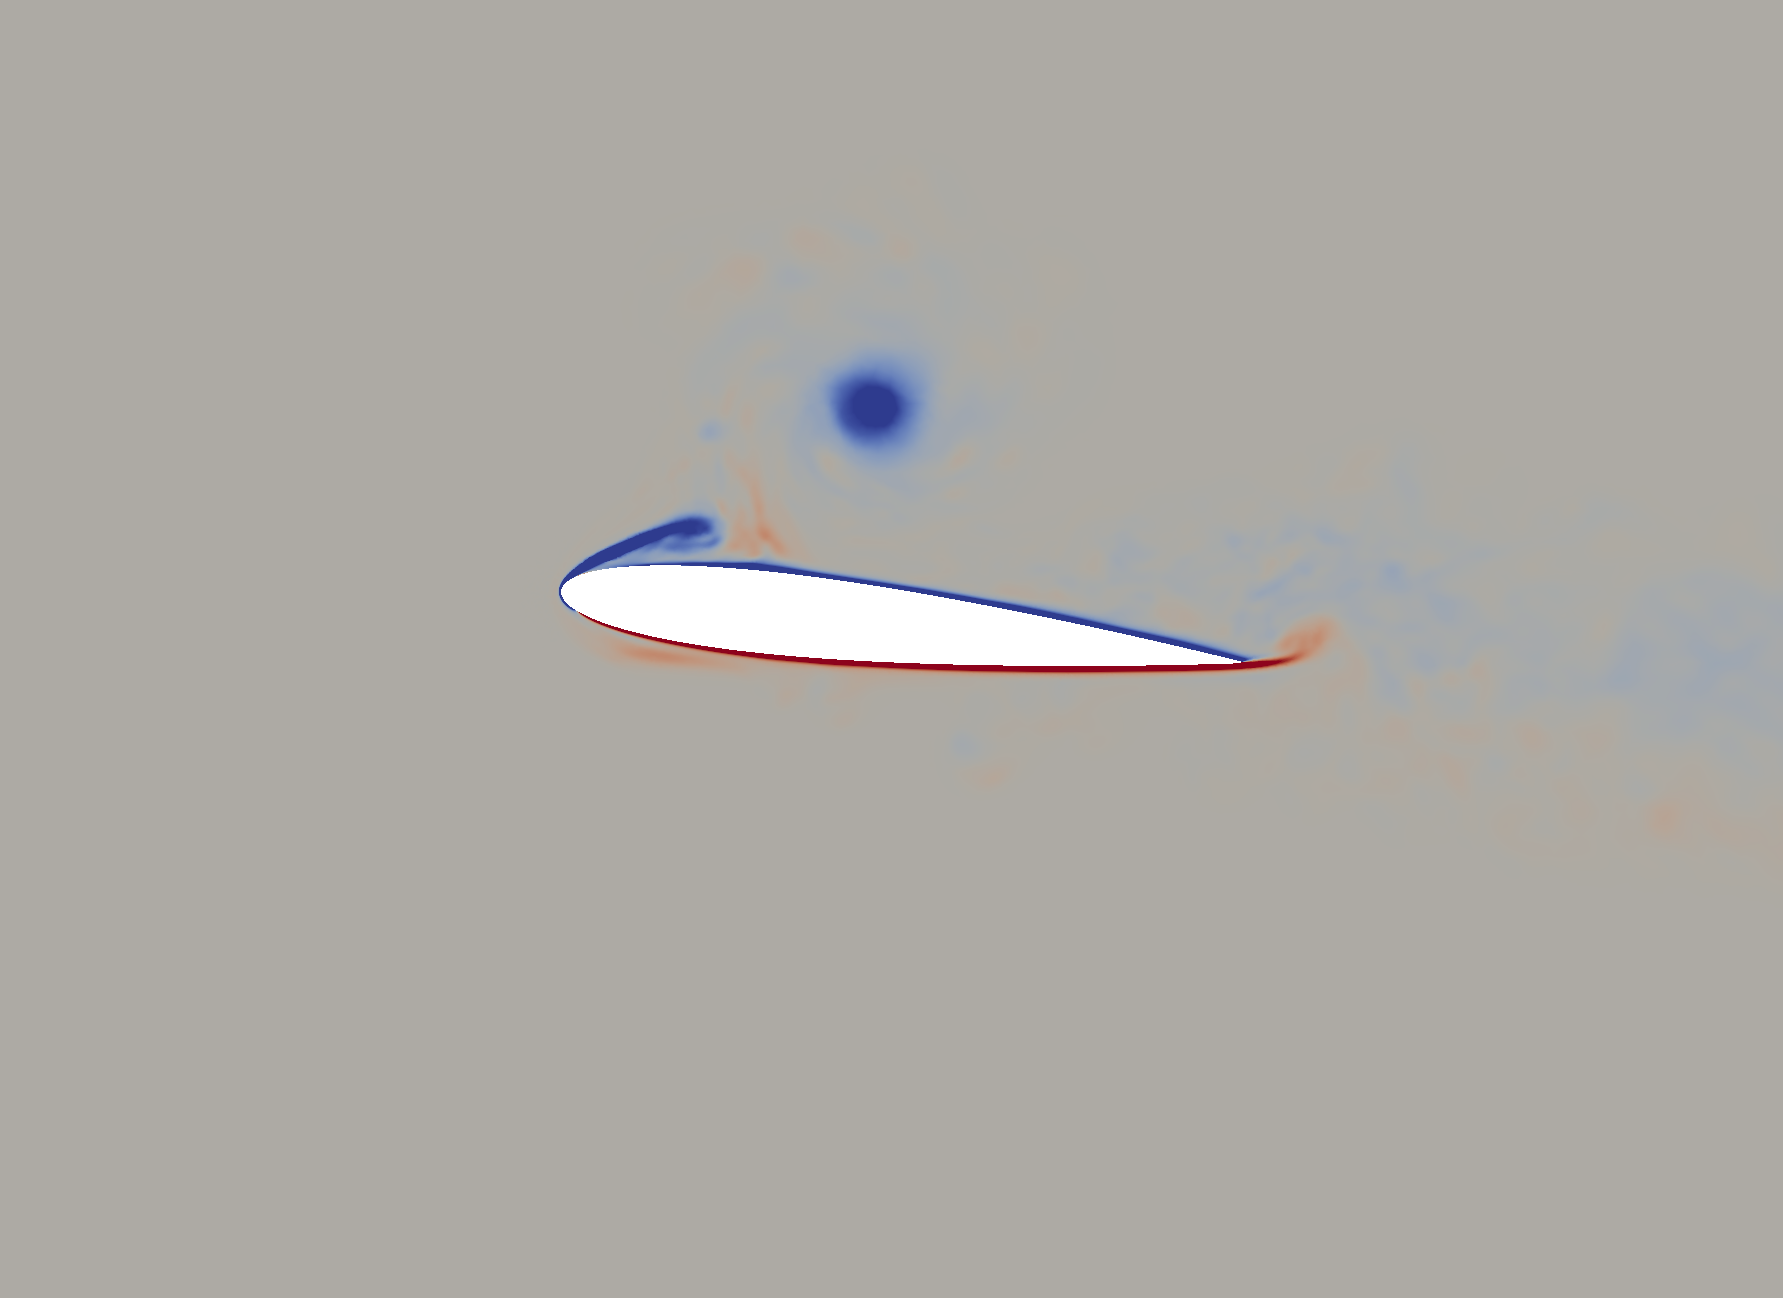
\includegraphics[width=1\textwidth]{figures/Vorticity_plots/Re_40k_1pt0/phase_315.png}
		\caption{$Re=4e4$, $\psi$ = $315^\circ$, $\tilde{t}=0.875$}
		\label{fig:Re_40k_1pt0_phi315}
	\end{subfigure}
	\begin{subfigure}[b]{0.32\textwidth}
		\centering
		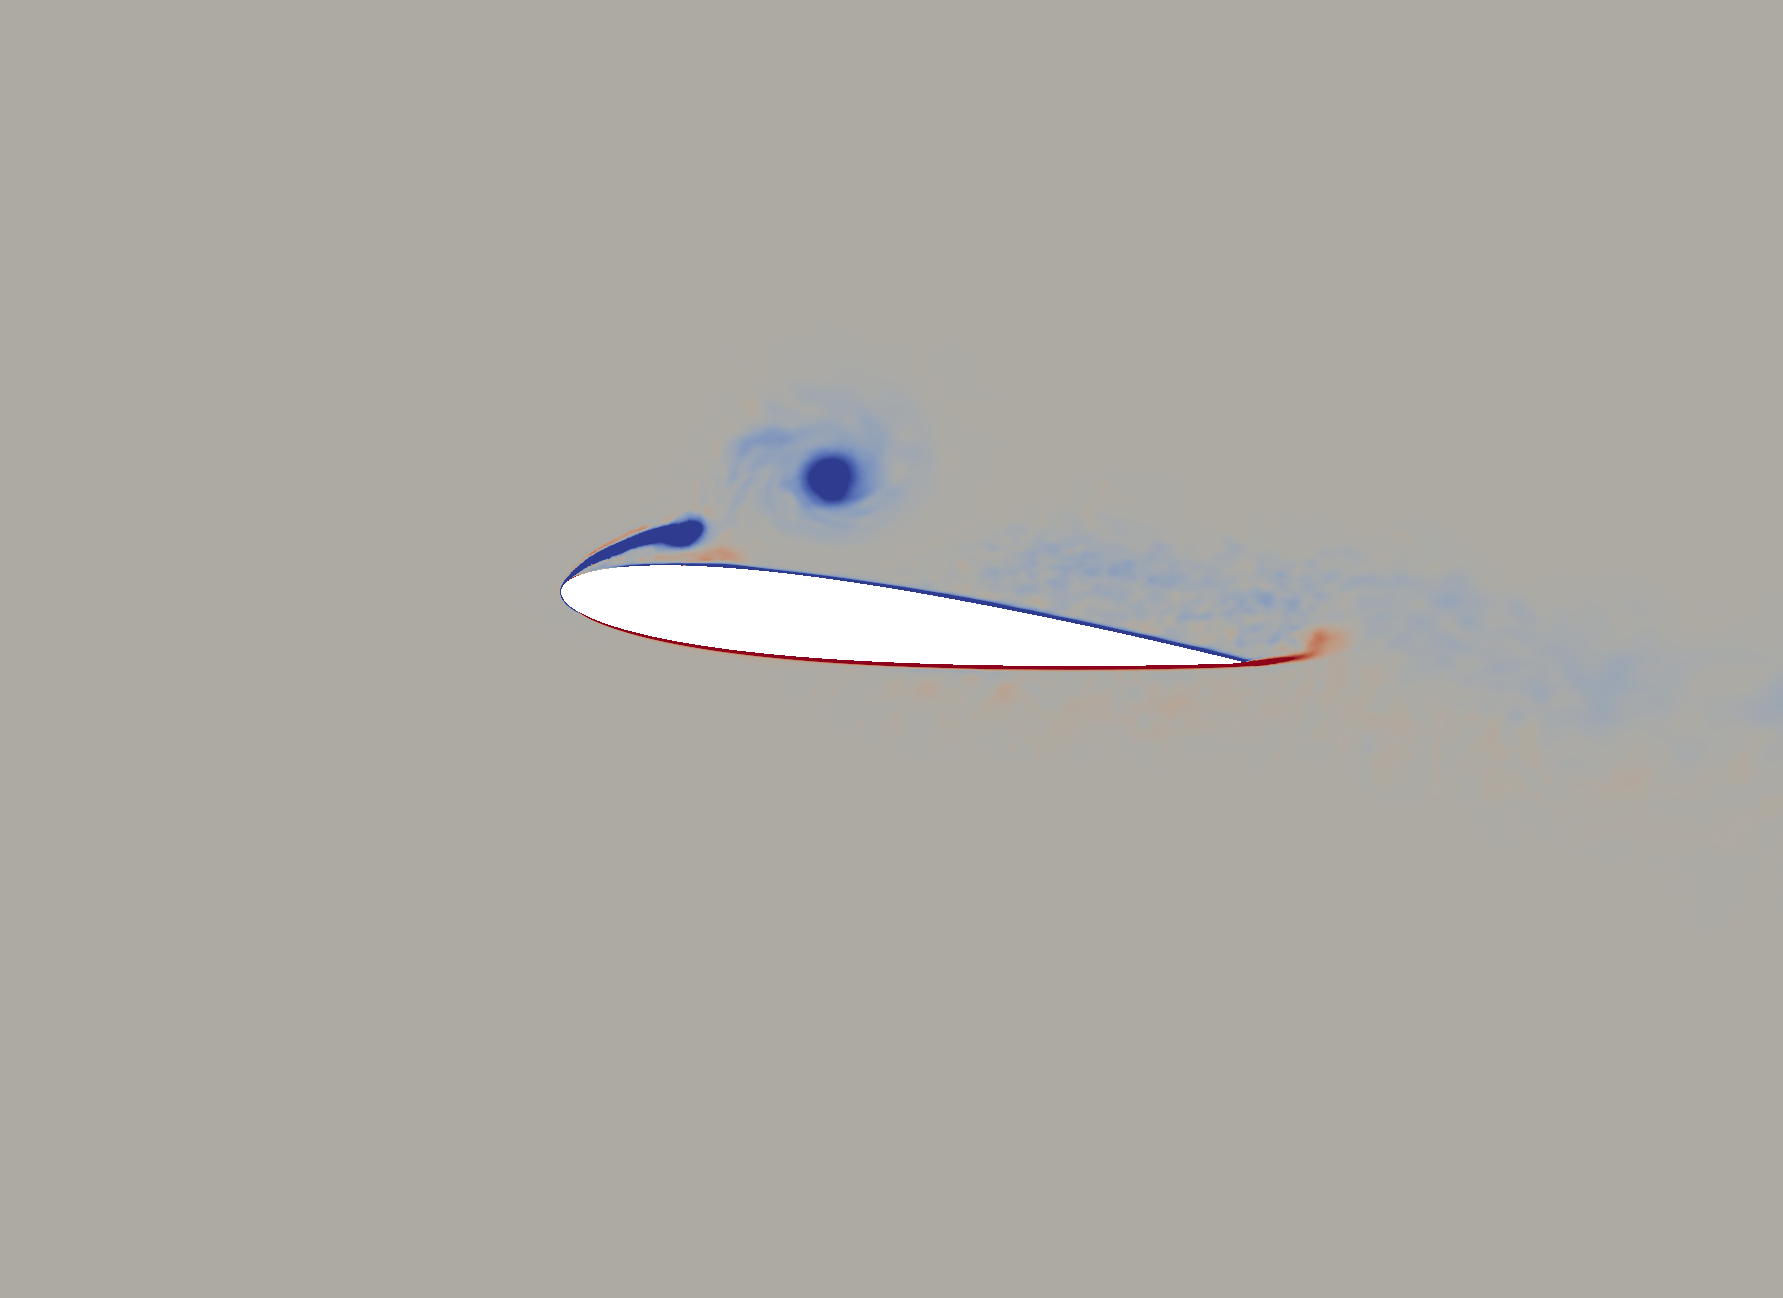
\includegraphics[width=1\textwidth]{figures/Vorticity_plots/Re_200k_1pt0/phase_315.png}
		\caption{$Re=2e5$, $\psi$ = $315^\circ$, $\tilde{t}=0.875$}
		\label{fig:Re_200k_1pt0_phi315}
	\end{subfigure}
	\begin{subfigure}[b]{0.32\textwidth}
		\centering
		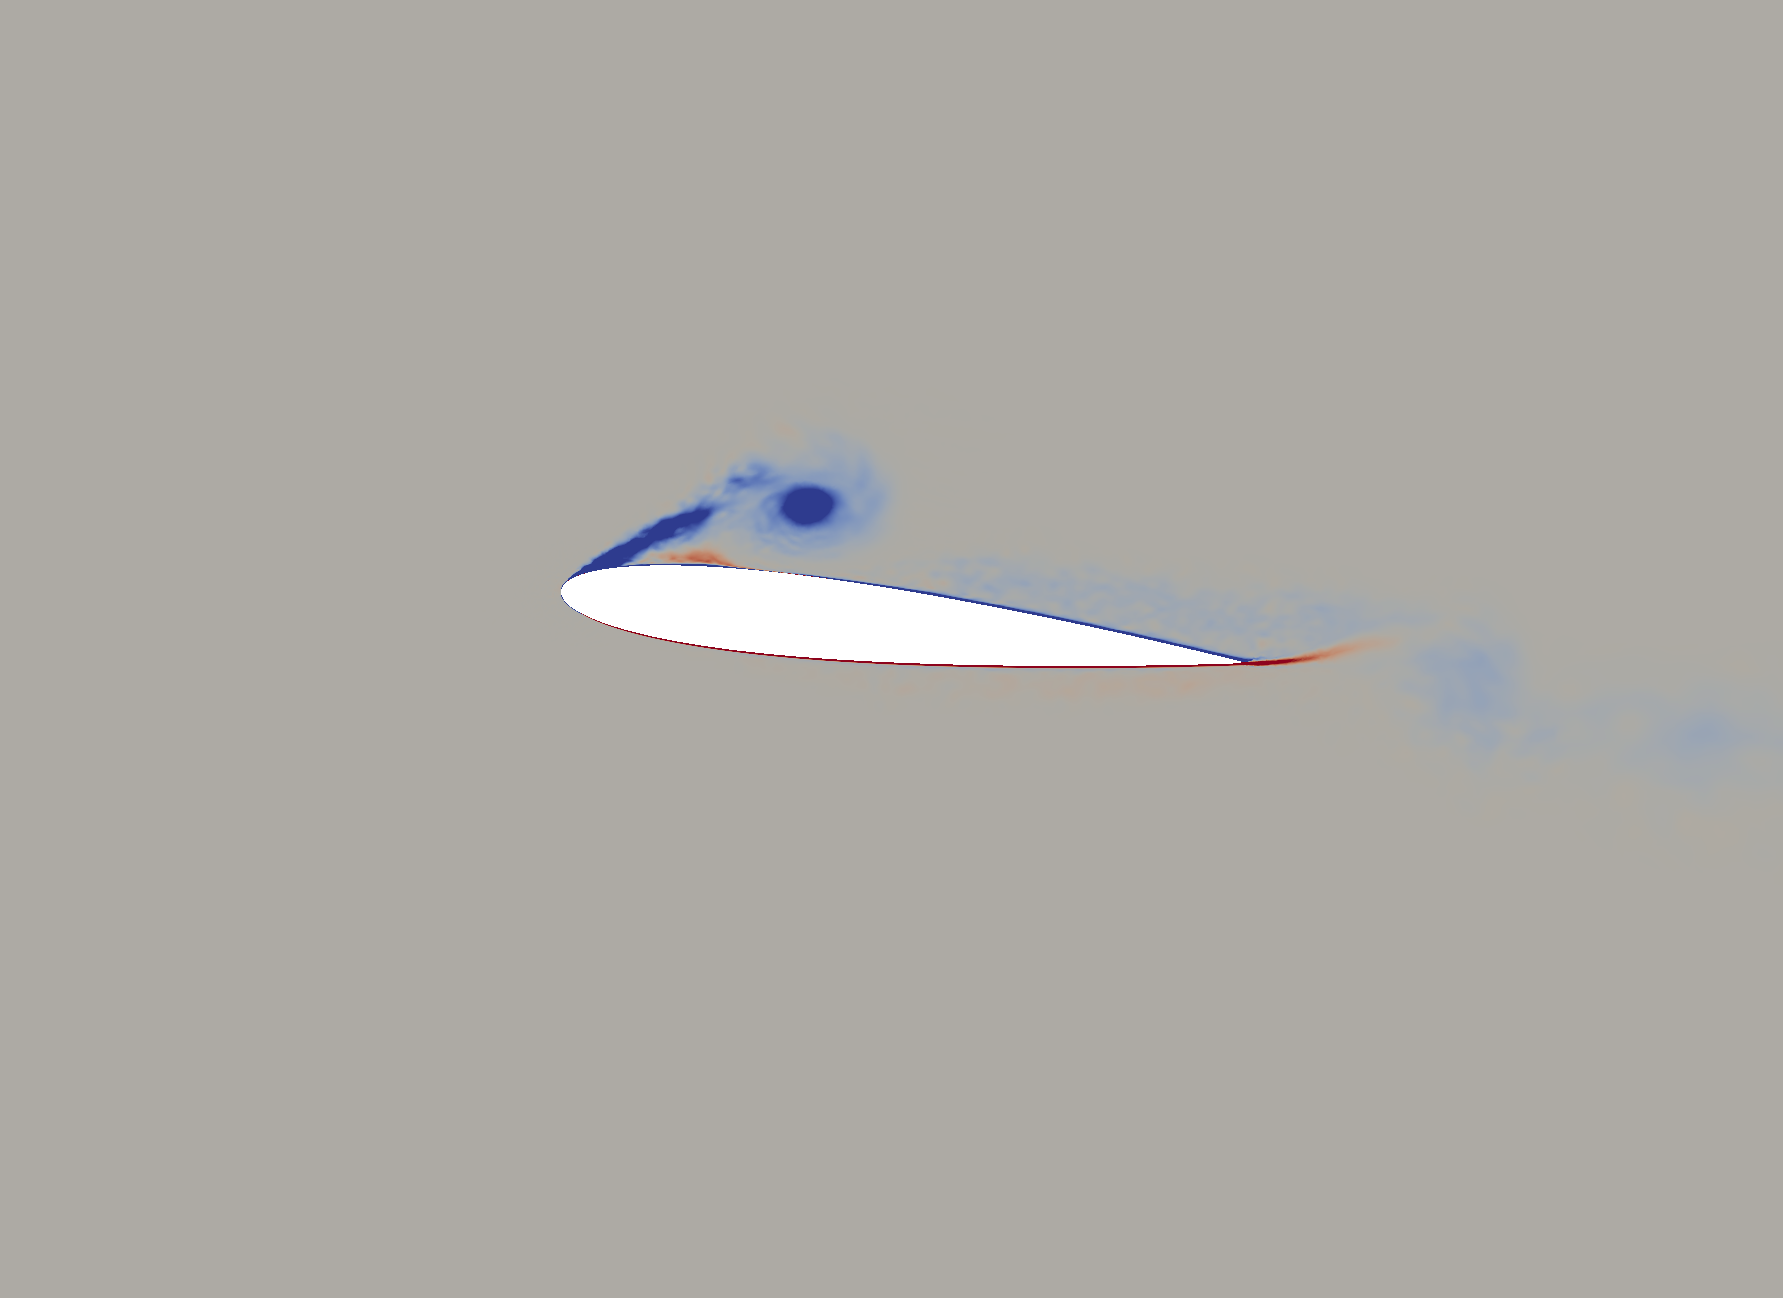
\includegraphics[width=1\textwidth]{figures/Vorticity_plots/Re_1m_1pt0/phase_315.png}
		\caption{$Re=1e6$, $\psi$ = $315^\circ$, $\tilde{t}=0.875$}
		\label{fig:Re_1m_1pt0_phi315}
	\end{subfigure}
	
	\begin{subfigure}[b]{0.32\textwidth}
		\centering
		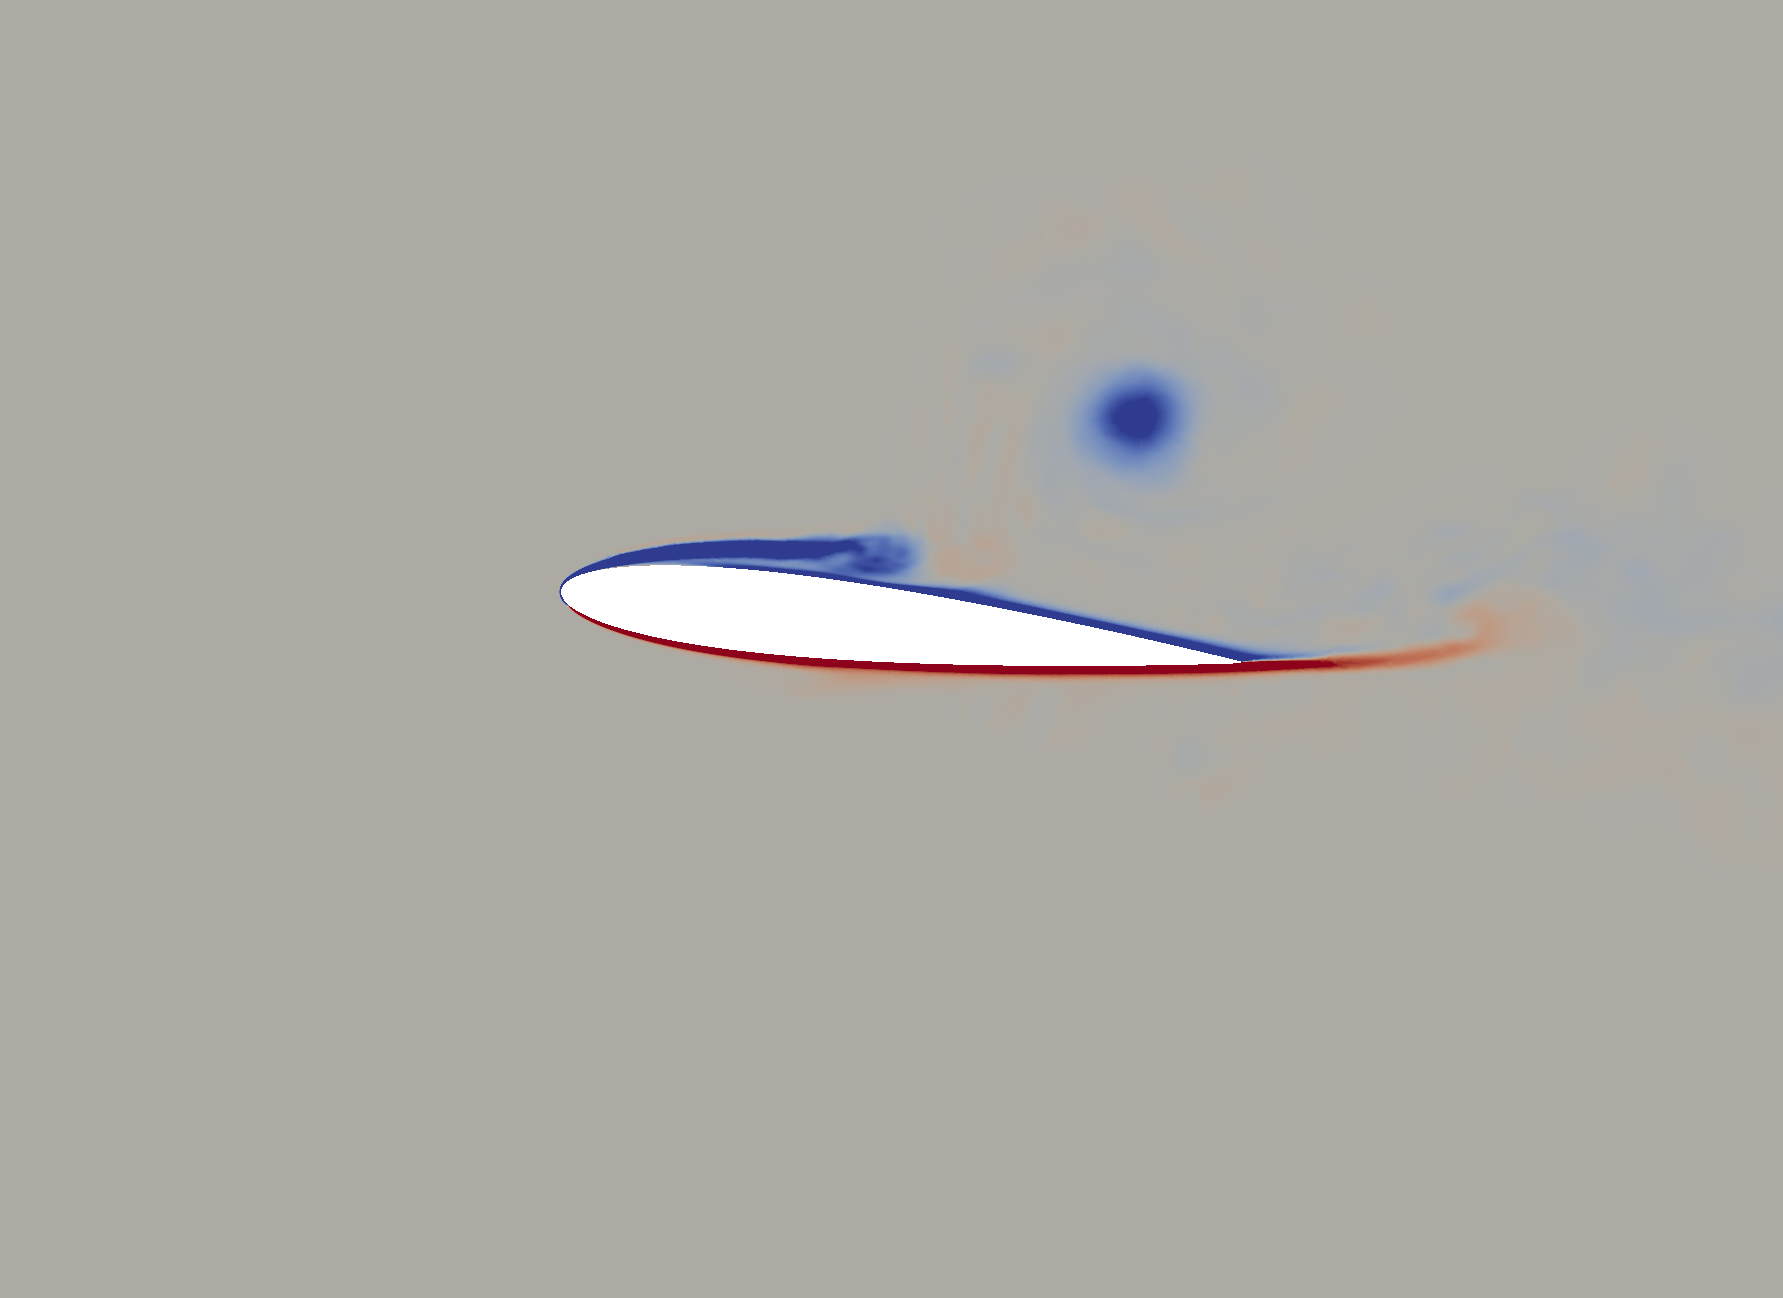
\includegraphics[width=1\textwidth]{figures/Vorticity_plots/Re_40k_1pt0/phase_330.png}
		\caption{$Re=4e4$, $\psi$ = $330^\circ$, $\tilde{t}=0.917$}
		\label{fig:Re_40k_1pt0_phi330}
	\end{subfigure}
	\begin{subfigure}[b]{0.32\textwidth}
		\centering
		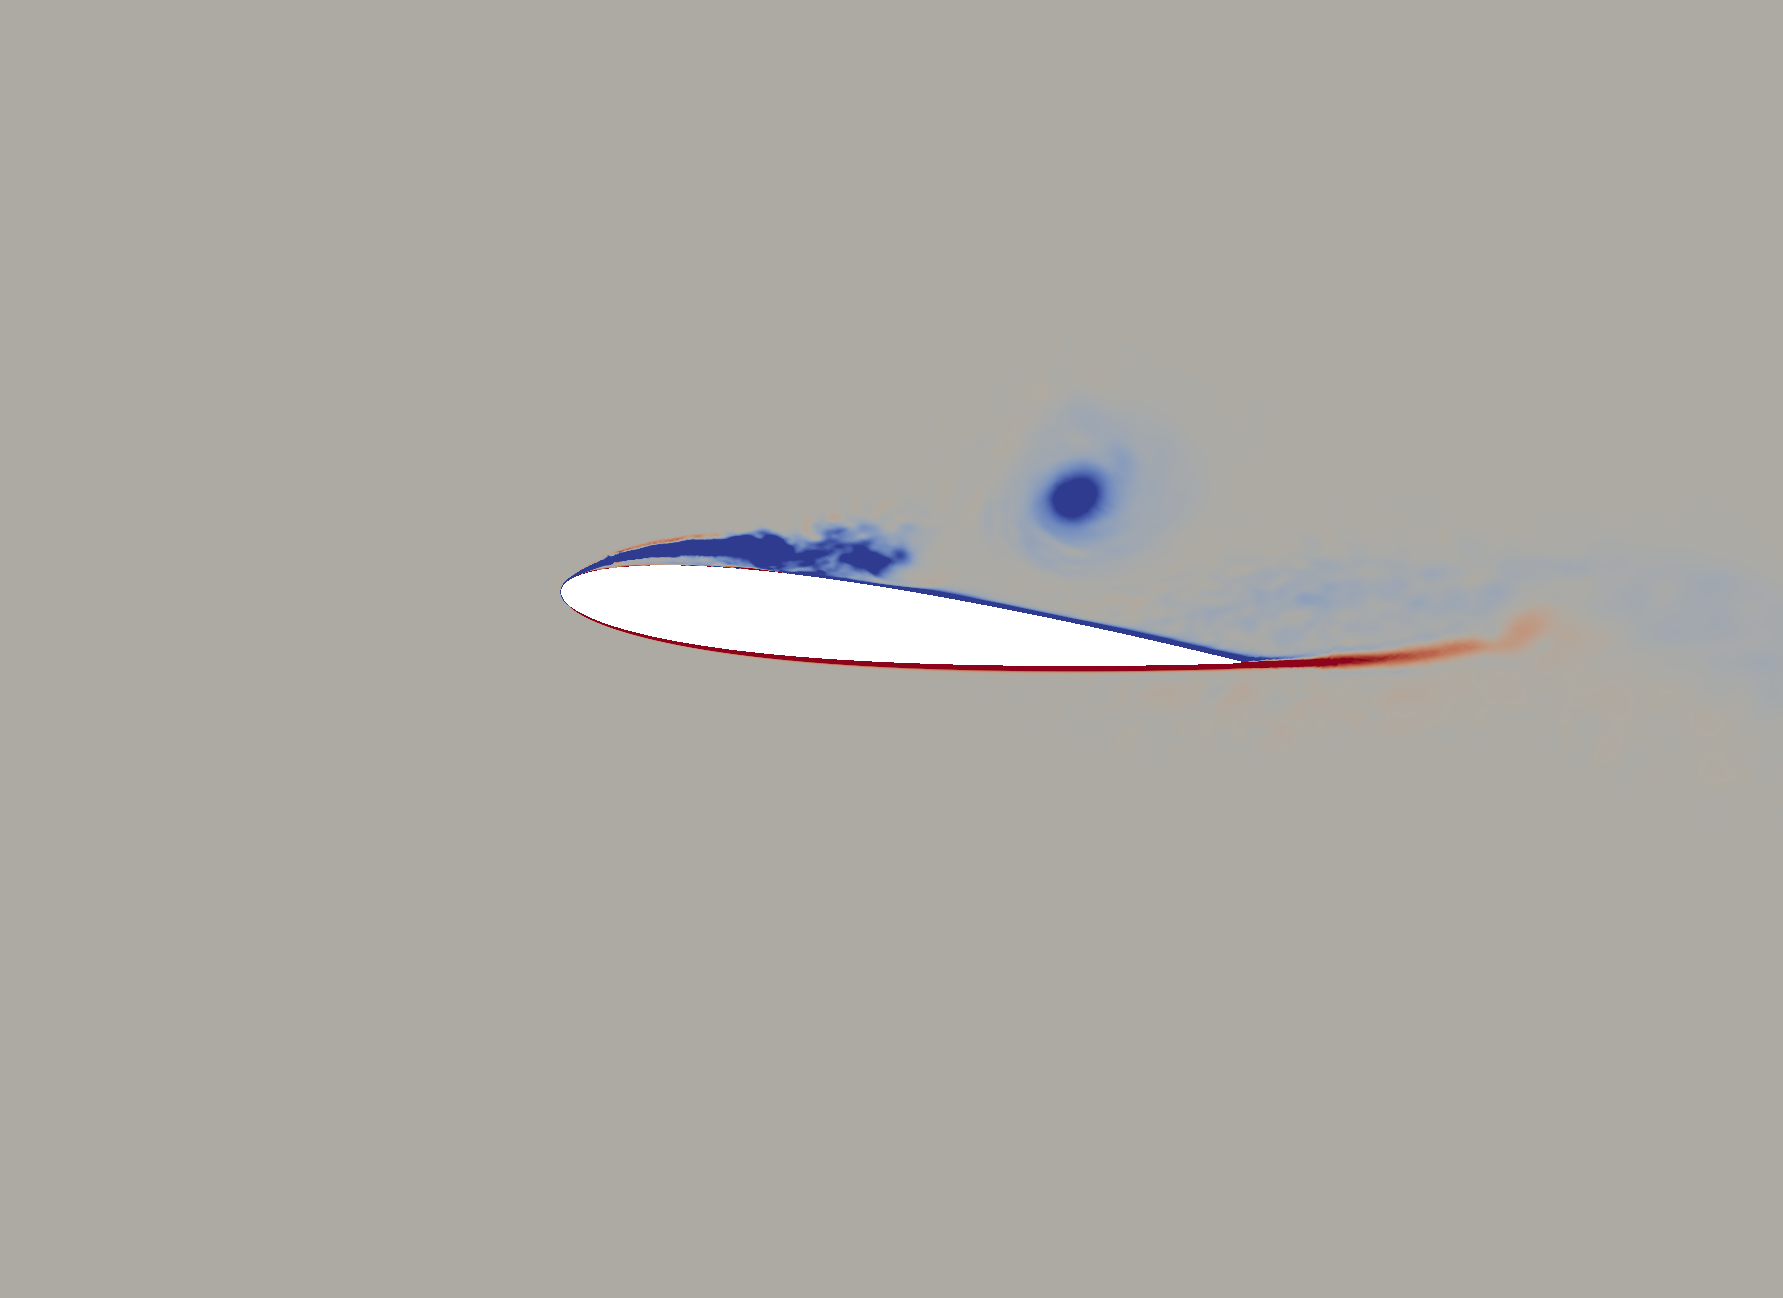
\includegraphics[width=1\textwidth]{figures/Vorticity_plots/Re_200k_1pt0/phase_330.png}
		\caption{$Re=2e5$, $\psi$ = $330^\circ$, $\tilde{t}=0.917$}
		\label{fig:Re_200k_1pt0_phi330}
	\end{subfigure}
	\begin{subfigure}[b]{0.32\textwidth}
		\centering
		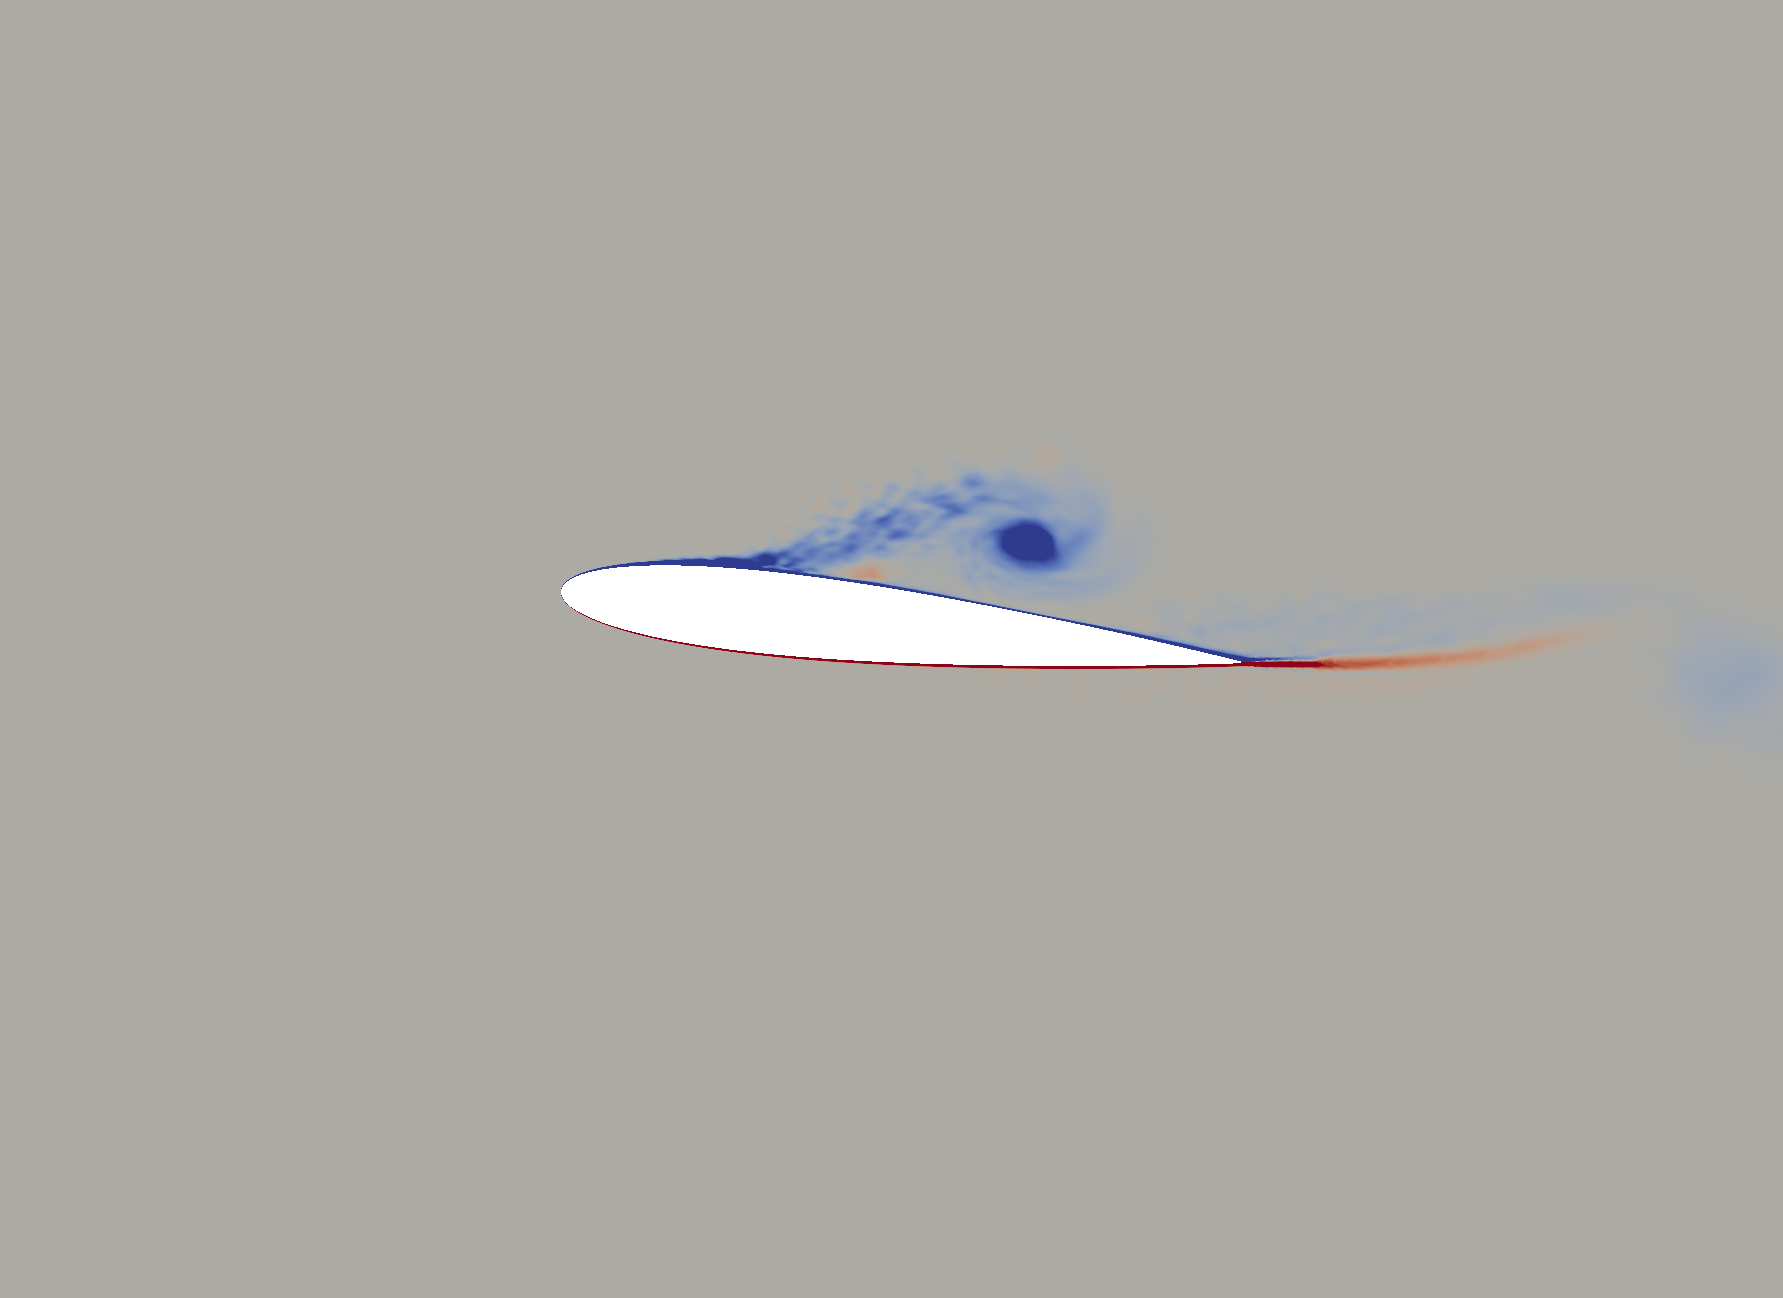
\includegraphics[width=1\textwidth]{figures/Vorticity_plots/Re_1m_1pt0/phase_330.png}
		\caption{$Re=1e6$,$\psi$ = $330^\circ$, $\tilde{t}=0.917$}
		\label{fig:Re_1m_1pt0_phi330}
	\end{subfigure}
	
	\begin{subfigure}[b]{0.32\textwidth}
		\centering
		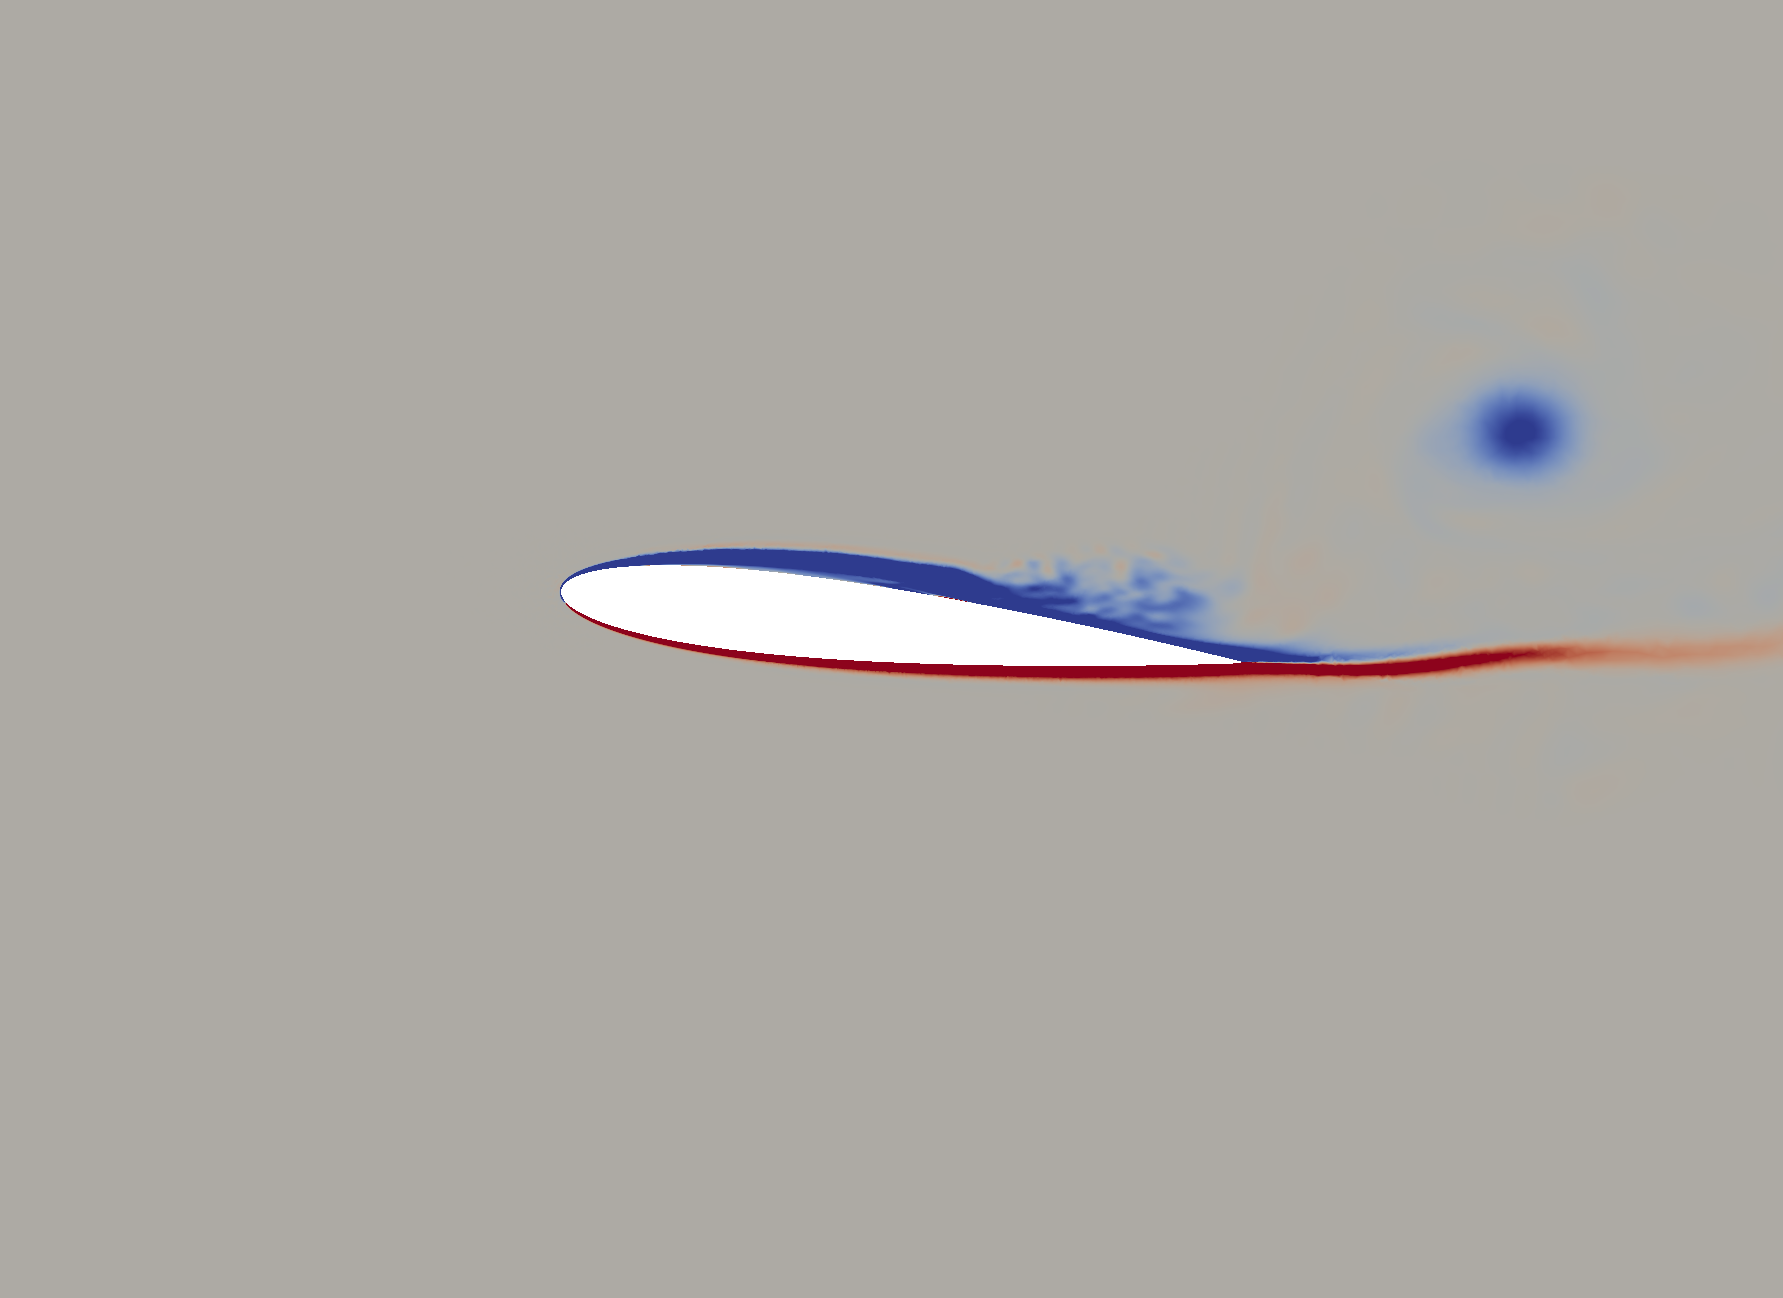
\includegraphics[width=1\textwidth]{figures/Vorticity_plots/Re_40k_1pt0/phase_345.png}
		\caption{$Re=4e4$, $\psi$ = $345^\circ$, $\tilde{t}=0.958$}
		\label{fig:Re_40k_1pt0_phi345}
	\end{subfigure}
	\begin{subfigure}[b]{0.32\textwidth}
		\centering
		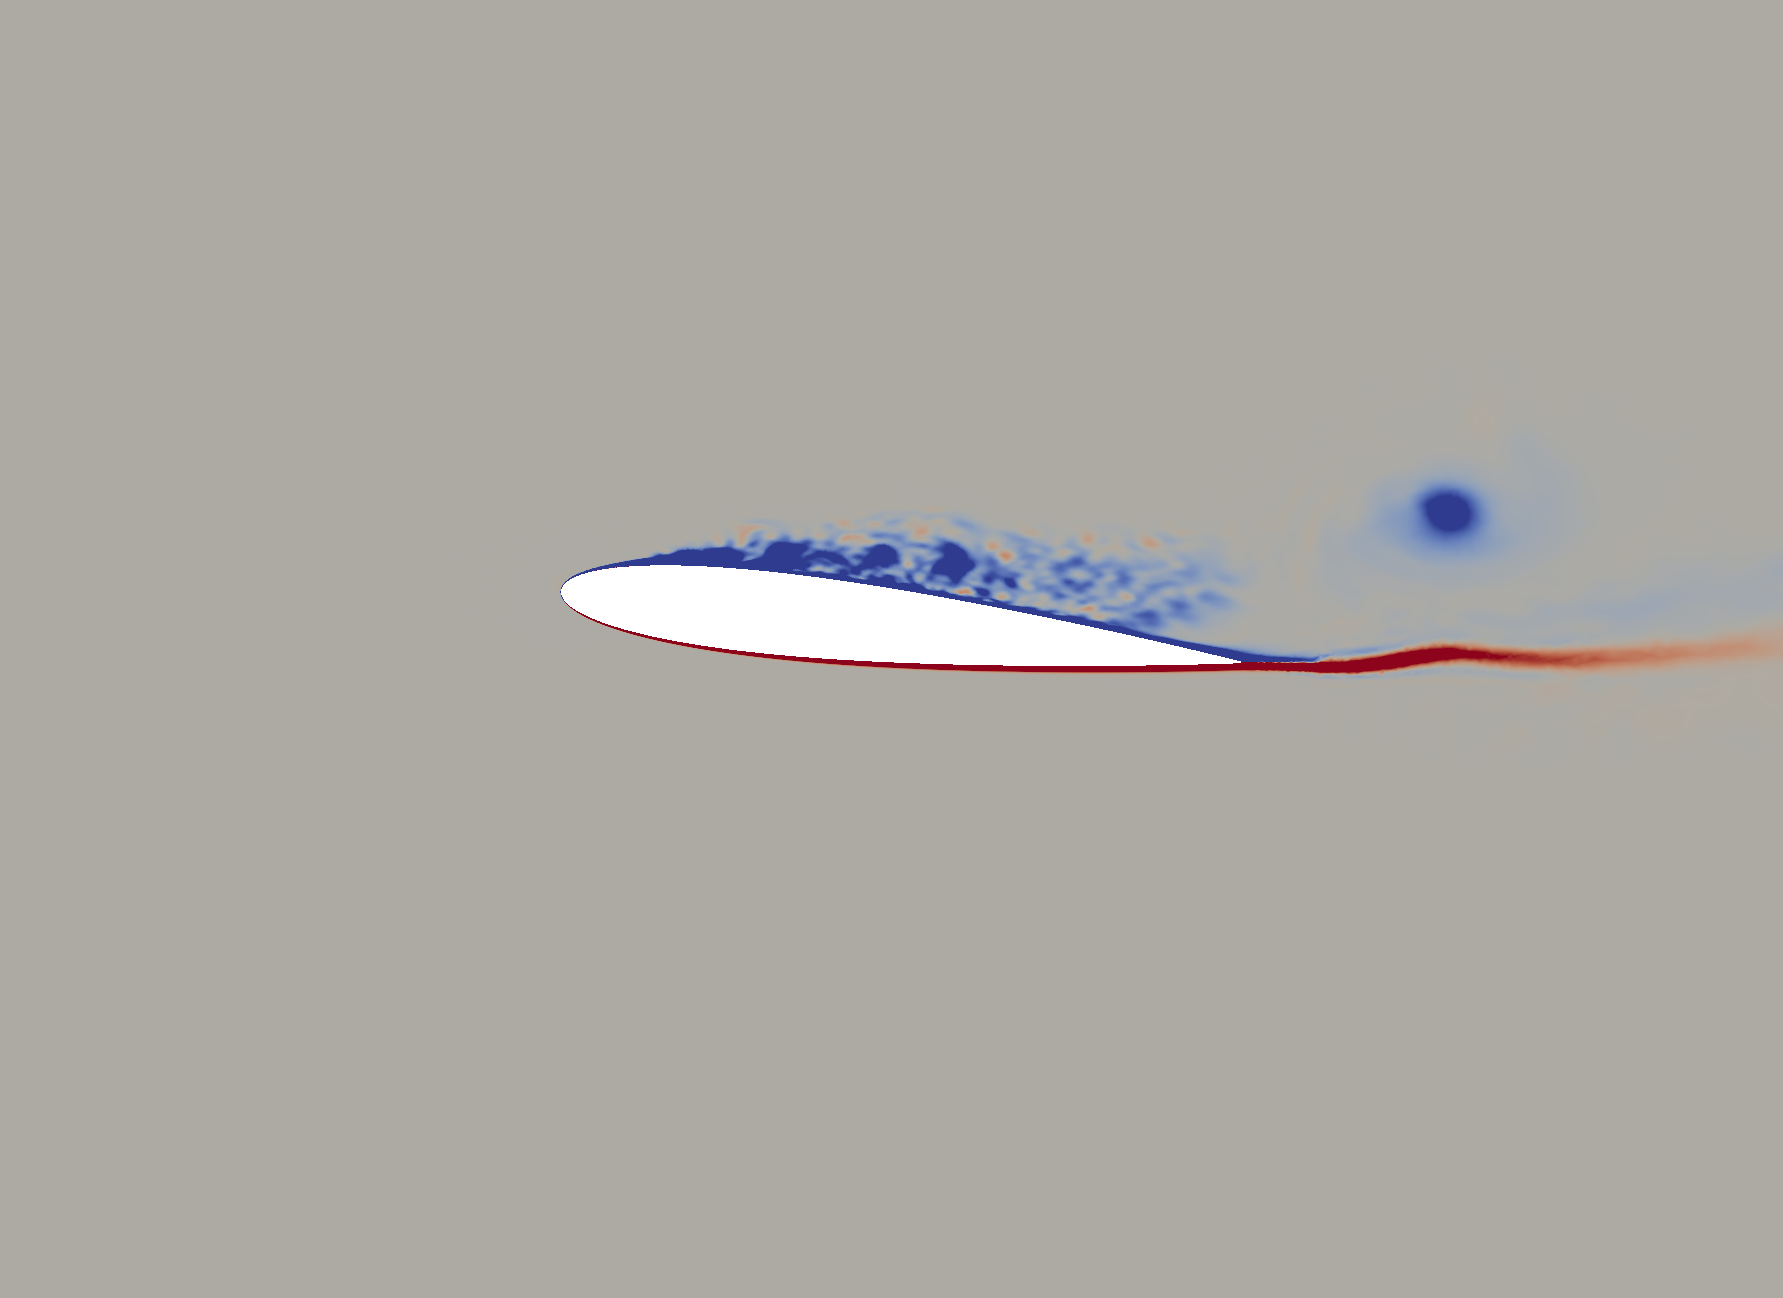
\includegraphics[width=1\textwidth]{figures/Vorticity_plots/Re_200k_1pt0/phase_345.png}
		\caption{$Re=2e5$, $\psi$ = $345^\circ$, $\tilde{t}=0.958$}
		\label{fig:Re_200k_1pt0_phi345}
	\end{subfigure}
	\begin{subfigure}[b]{0.32\textwidth}
		\centering
		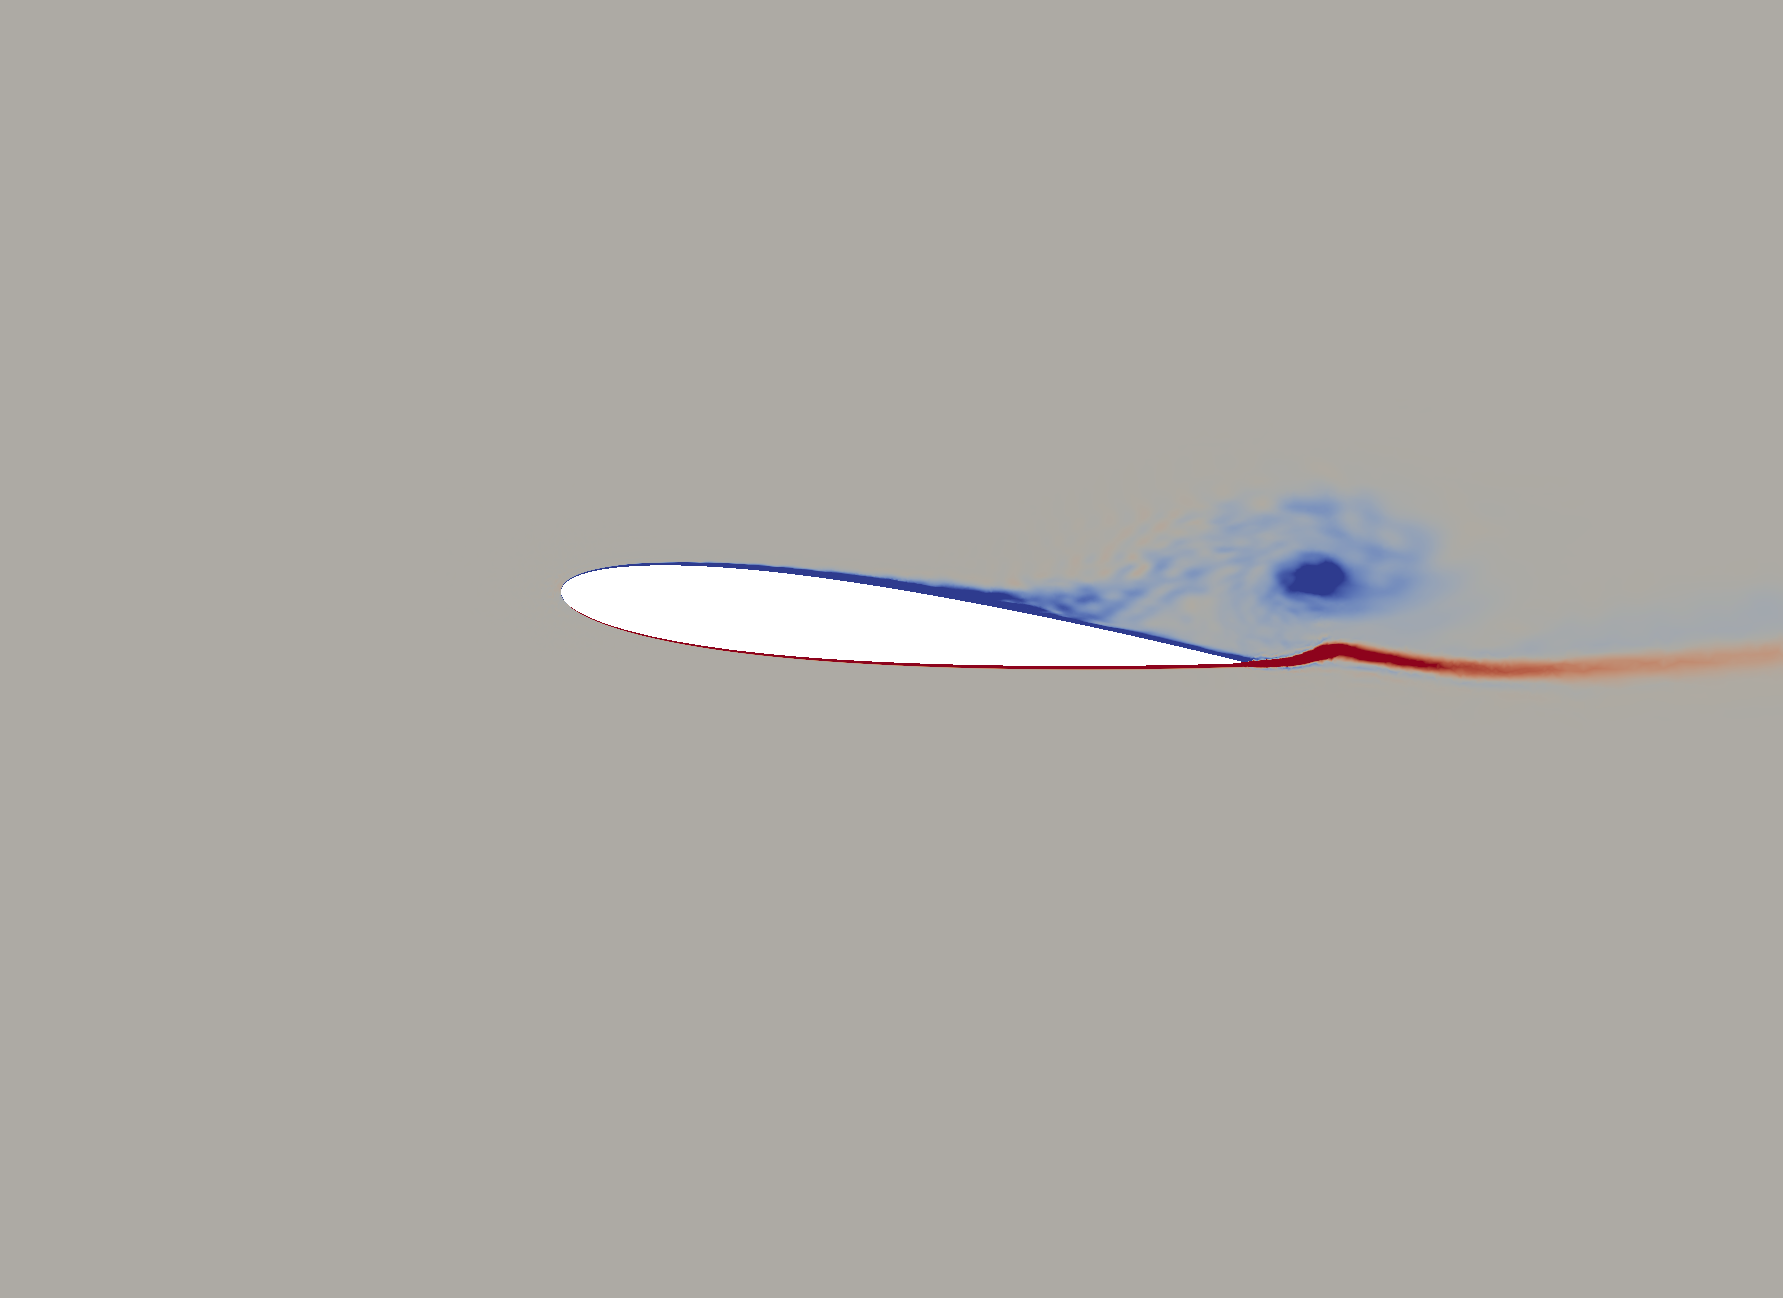
\includegraphics[width=1\textwidth]{figures/Vorticity_plots/Re_1m_1pt0/phase_345.png}
		\caption{$Re=1e6$, $\psi$ = $345^\circ$, $\tilde{t}=0.958$}
		\label{fig:Re_1m_1pt0_phi345}
	\end{subfigure}	
\caption{Spanwise vorticity at 8 different phases for $Re$=40,000 (left column), 200,000 (middle column) and 1,000,000 (right column) at $\lambda$ = 1.0}
\label{fig:vortScreen_1pt0}
\end{figure}


At $\psi$=$225^\circ$, the flow is separated near the leading edge for the lowest Reynolds number of $Re$=40,000 and the separated shear layer rolls up into an LEV, see Figure~\ref{fig:Re_200k_1pt0_phi225}
For the other two higher Reynolds number, the flow remains attached.
Similarly, at $Re$=200,000 the separated shear layer rolls up into a small LEV at $\psi$=$240^\circ$, while for $Re$=1,000,000 this occurs at $\psi$=$270^\circ$ (see Figure \ref{fig:Re_1m_1pt0_phi270}).
As the Reynolds number increases the LEV is formed later in the cycle.
In summary, as the airfoil retreats vorticity accumulates around the airfoil and separated shear layer rolls up into a distinct vortex near the leading edge (i.e., an LEV) over the suction or upper side of the airfoil.

In subsequent phases, LEV is ejected into the outer flow and advects.
The flow on the suction or upper side reattaches as the leading edge vortex passes over the airfoil.
Flow also separates and reattaches on the pressure or lower side, e.g., see marginal flow separation at the trailing edge on the lower side in Fig \ref{fig:Re_40k_1pt0_phi225}.

It is important to note the differences in LEV evolution with different Reynolds number even though the overall trend of the LEV evolution is similar between different Reynolds number.
As already noted, the phase at which the LEV is formed changes with Reynolds number.
Further, the size and vertical position of the LEV also changes significantly with Reynolds number.
This aspect is discussed in Section \ref{sec:LEV}.

Figure \ref{fig:vortScreen_1pt2} shows the spanwise vorticity for the higher advance ratio of $\mu_{sect}$=1.2.
3 different phases over the retreating phase of the cycle are shown and the range is selected to be [-10,10]$\times U_\infty /C$.
As in the $\mu_{sect}=1.0$ case, at $\psi$=$195^\circ$ the flow over the airfoil is mostly attached in the $\mu_{sect}=1.2$ case.
As before, the boundary layer is much thicker for the lowest Reynolds number of $Re$=40,000 as compared to the other two higher Reynolds number.

At $\psi$=$225^\circ$, the flow is fully separated for the lowest Reynolds number of $Re$=40,000 and the separated shear layer is rolled up into an LEV, see Figure~\ref{fig:Re_40k_1pt2_phi225}.
Similarly, at $Re$=200,000 a small LEV is seen at $\psi$=$225^\circ$ (see Figure \ref{fig:Re_200k_1pt2_phi225}) while for $Re$=1,000,000 LEV is observed at $\psi$=$240^\circ$.
As before, as the Reynolds number increases the LEV is formed later in the cycle.
On the other hand, as the advance ratio increases it is formed earlier in the cycle (for a given Reynolds number).
For example, for $Re$=1,000,000, the LEV is formed at an earlier phase for $\mu_{sect}=1.2$ as compared to $\mu_{sect}=1.0$.
Again, as the airfoil retreats vorticity accumulates and shear layer rolls up into a distinct LEV over the suction or upper side of the airfoil.

In subsequent phases, LEV is ejected into the outer flow and advects while the flow reattaches.
However, at the higher advance ratio of $\mu_{sect}$=1.2 the LEV initially moves to the left past the (geometric) leading edge of the airfoil.
This is because at $\mu_{sect}$=1.2 the relative flow velocity becomes negative and a reversed flow condition is reached.
Again, it is important to note the differences in LEV evolution with different Reynolds number for the advance ratio of $\mu_{sect}=1.2$.
As already noted, the size, position and phase of formation of LEV changes significantly with Reynolds number.
This aspect is discussed further in Section \ref{sec:LEV}.

\begin{figure}[H]
	\centering
	
	\begin{subfigure}[b]{0.32\textwidth}
		\centering
		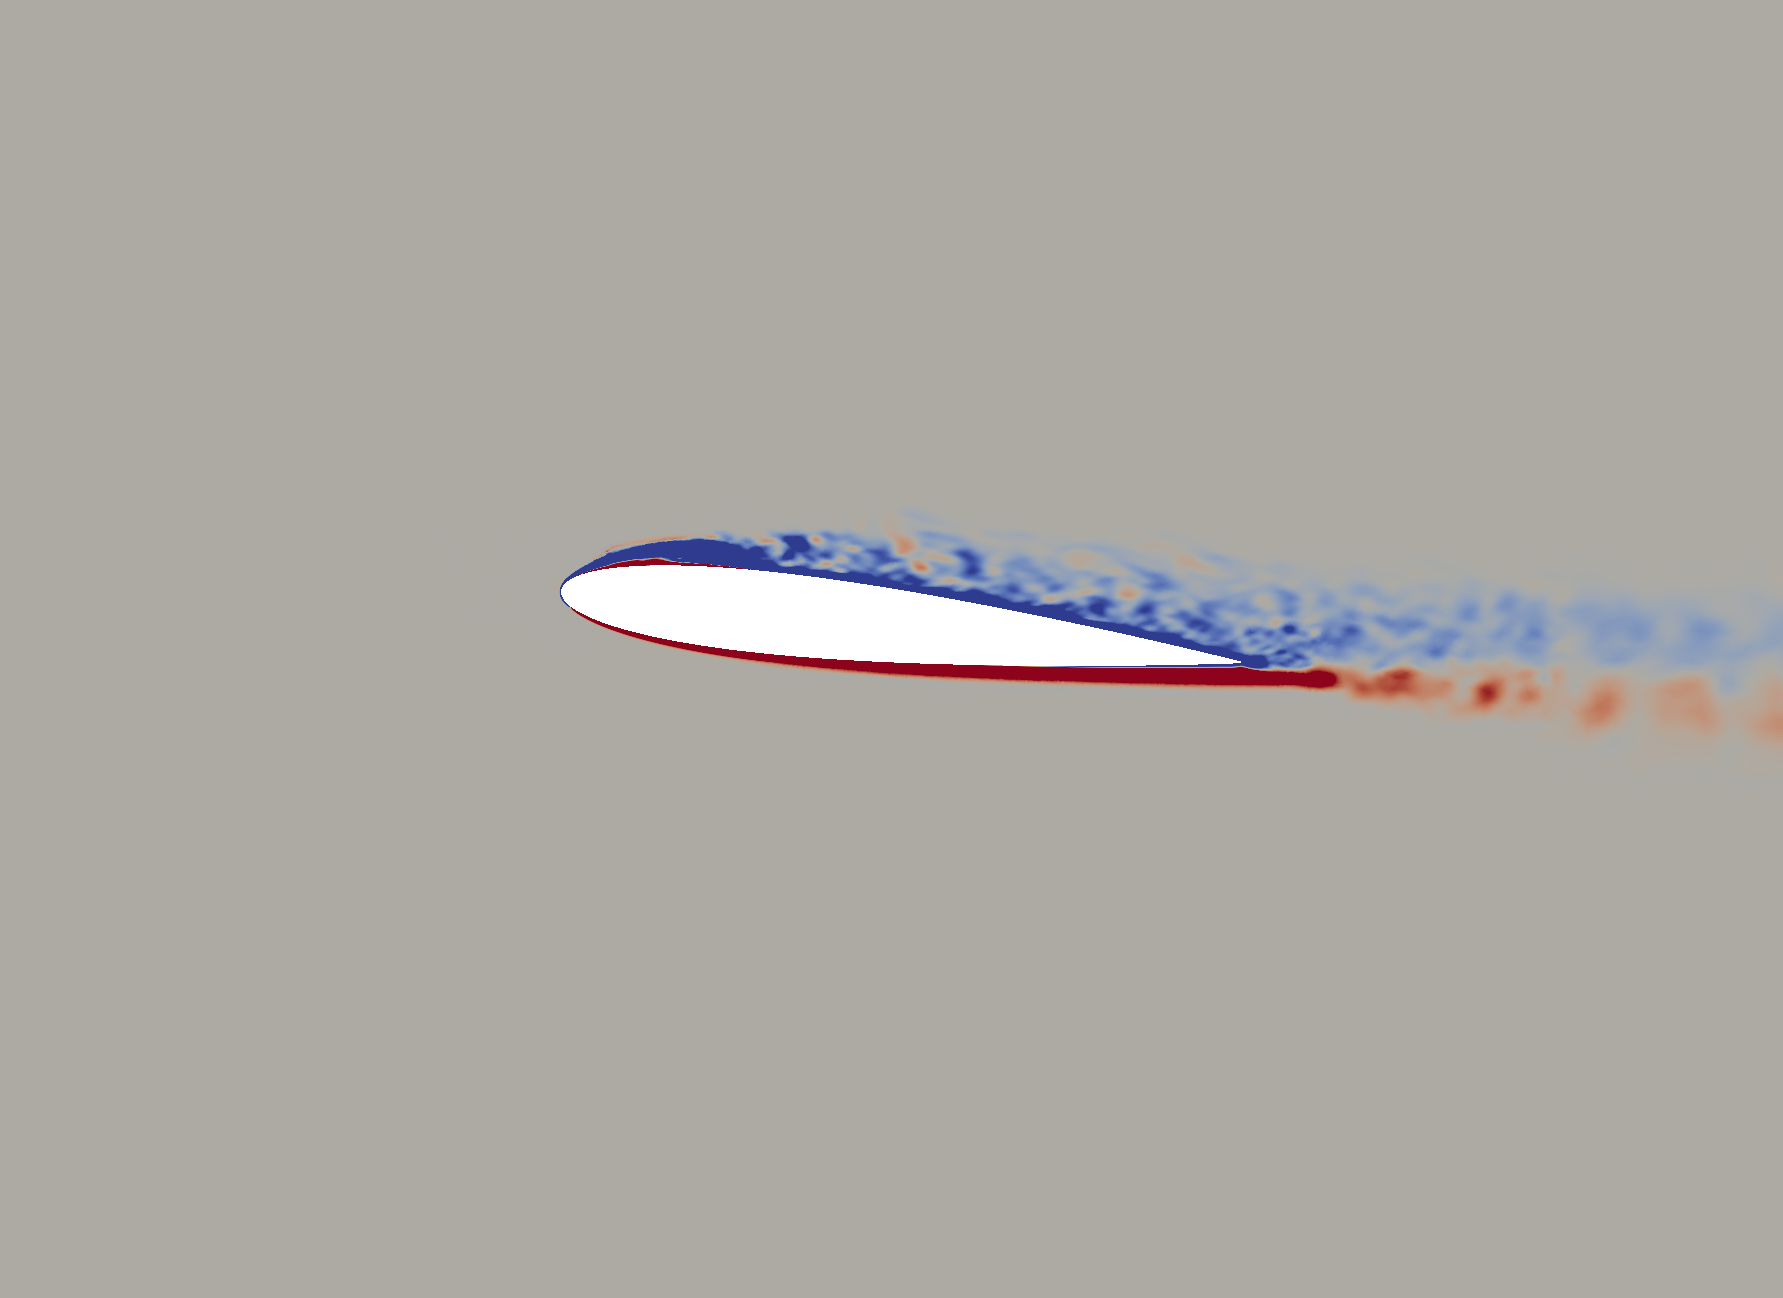
\includegraphics[width=1\textwidth]{figures/Vorticity_plots/Re_40k_1pt2/phase_195.png}
		\caption{$Re= 4e4$, $\psi$ = $195^\circ$, $\tilde{t}=0.542$}
		\label{fig:Re_40k_1pt2_phi195}
	\end{subfigure}
	\begin{subfigure}[b]{0.32\textwidth}
		\centering
		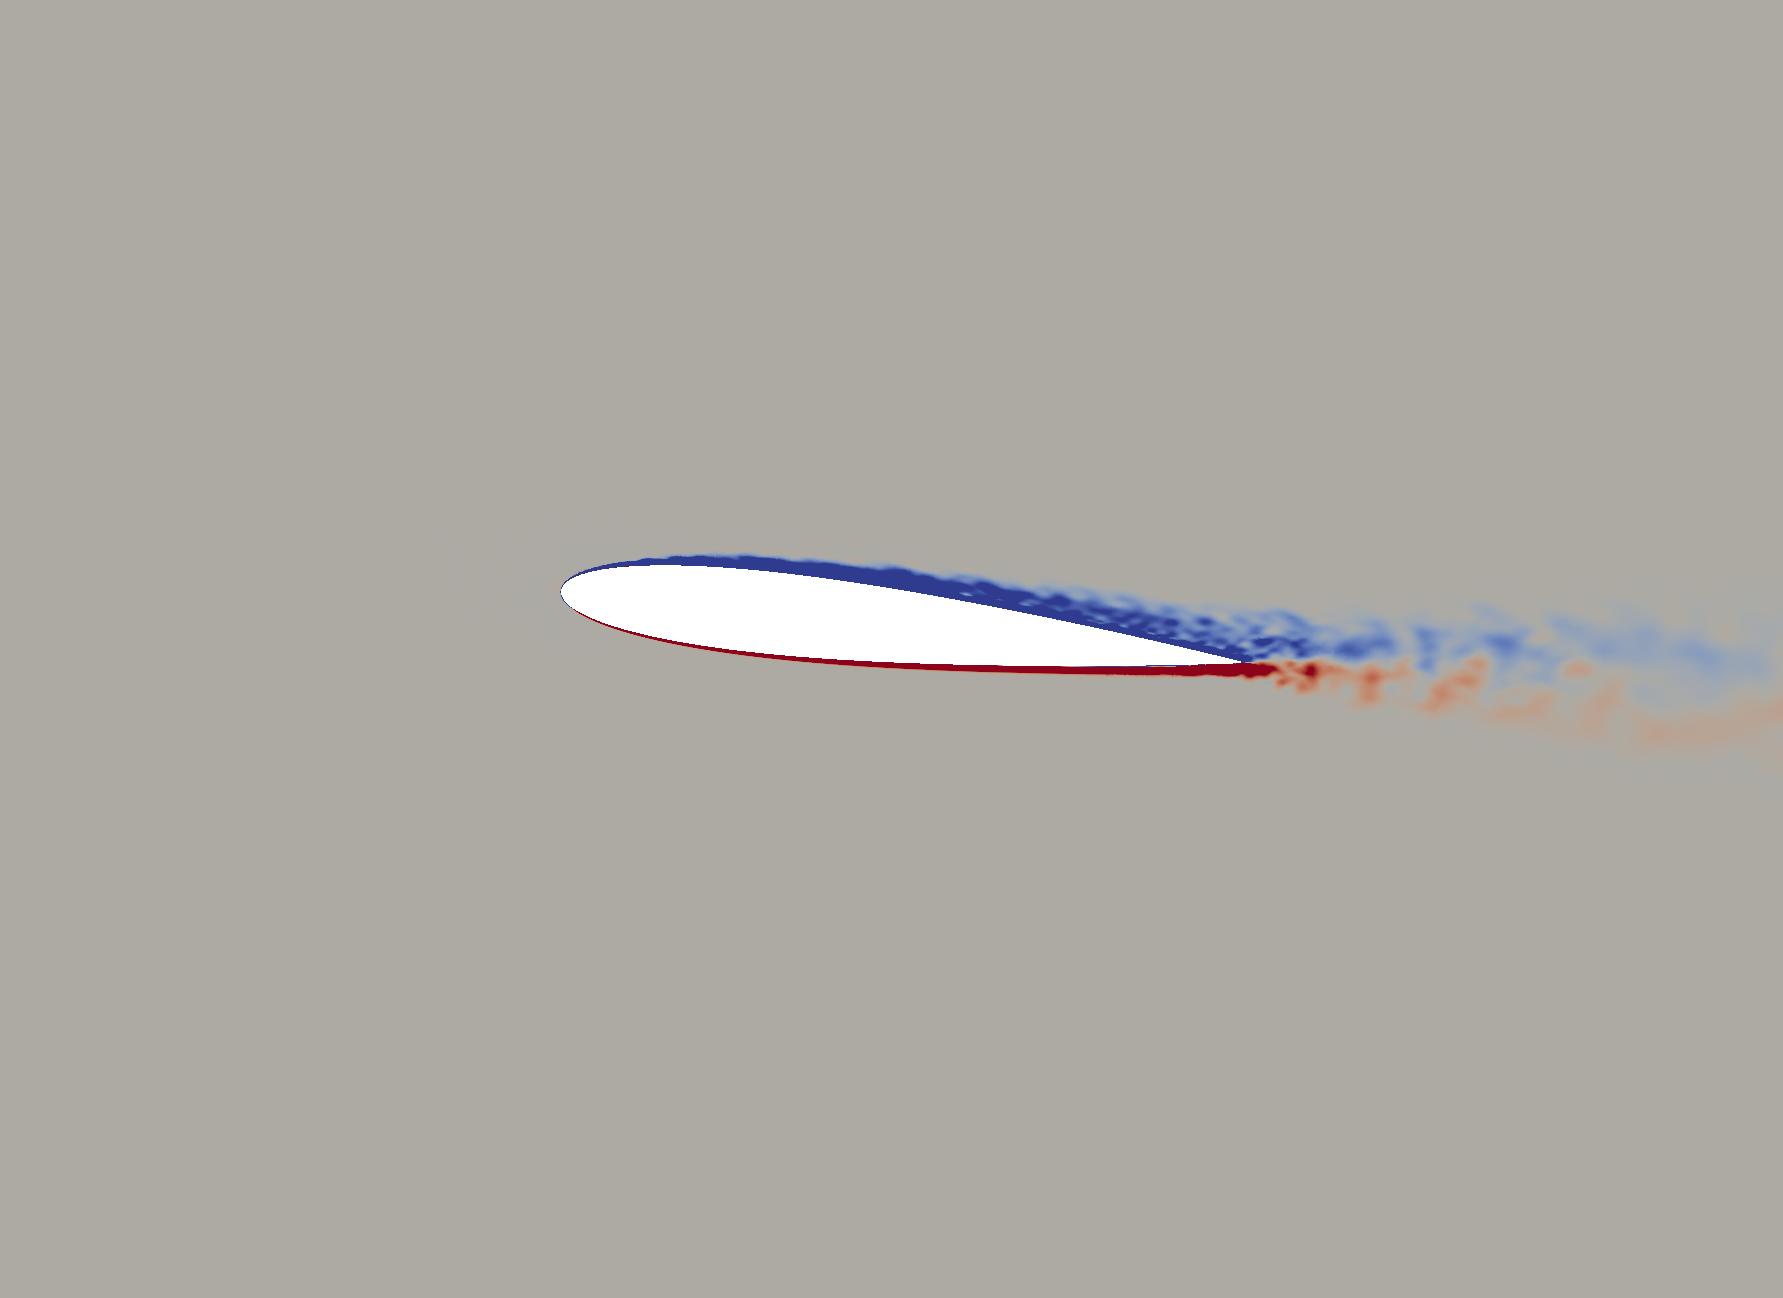
\includegraphics[width=1\textwidth]{figures/Vorticity_plots/Re_200k_1pt2/phase_195.png}
		\caption{$Re=2e5$, $\psi$ = $195^\circ$, $\tilde{t}=0.542$}
		\label{fig:Re_200k_1pt2_phi195}
	\end{subfigure}
	\begin{subfigure}[b]{0.32\textwidth}
		\centering
		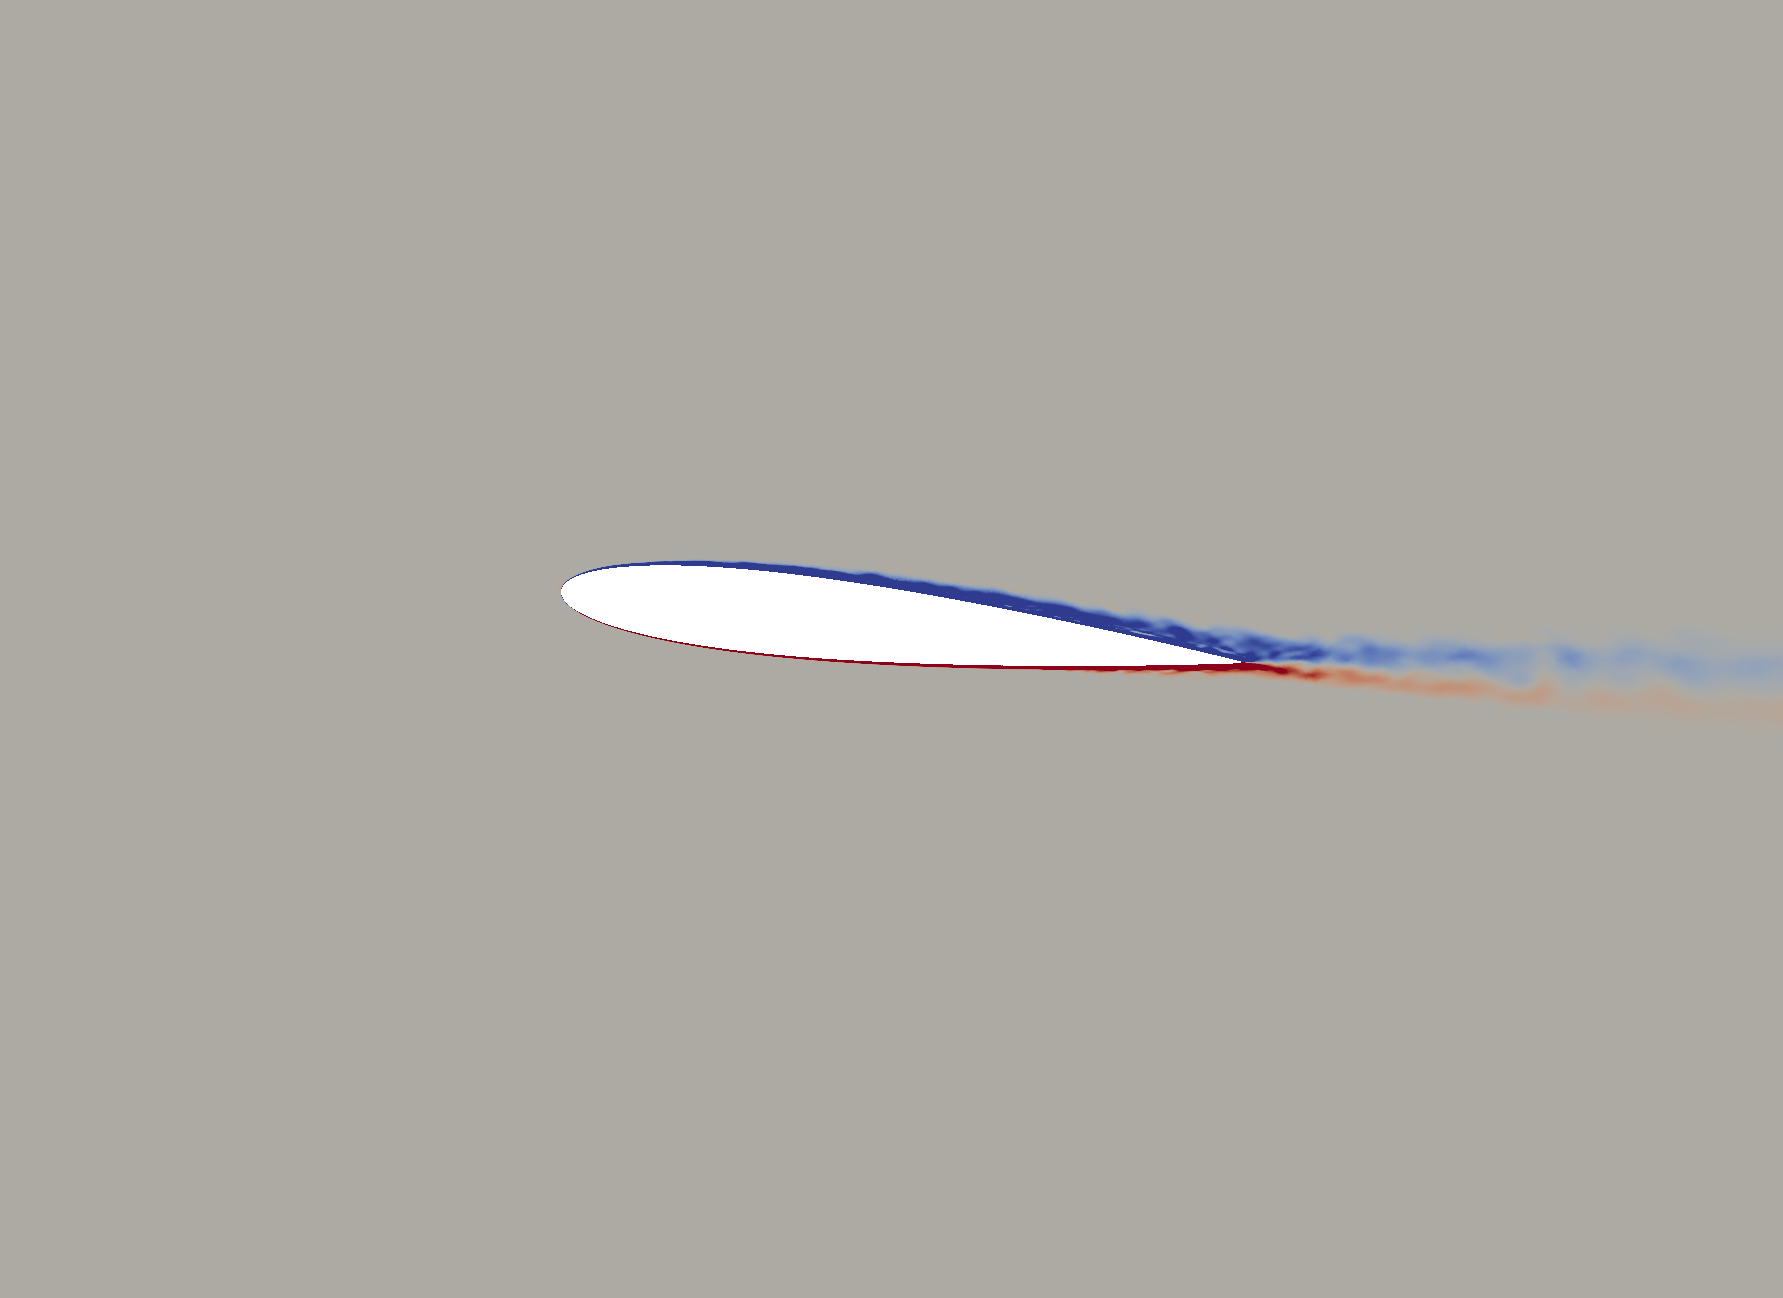
\includegraphics[width=1\textwidth]{figures/Vorticity_plots/Re_1m_1pt2/phase_195.png}
		\caption{$Re= 1e6$, $\psi$ = $195^\circ$, $\tilde{t}=0.542$}
		\label{fig:Re_1m_1pt2_phi195}
	\end{subfigure}
	
	\begin{subfigure}[b]{0.32\textwidth}
		\centering
		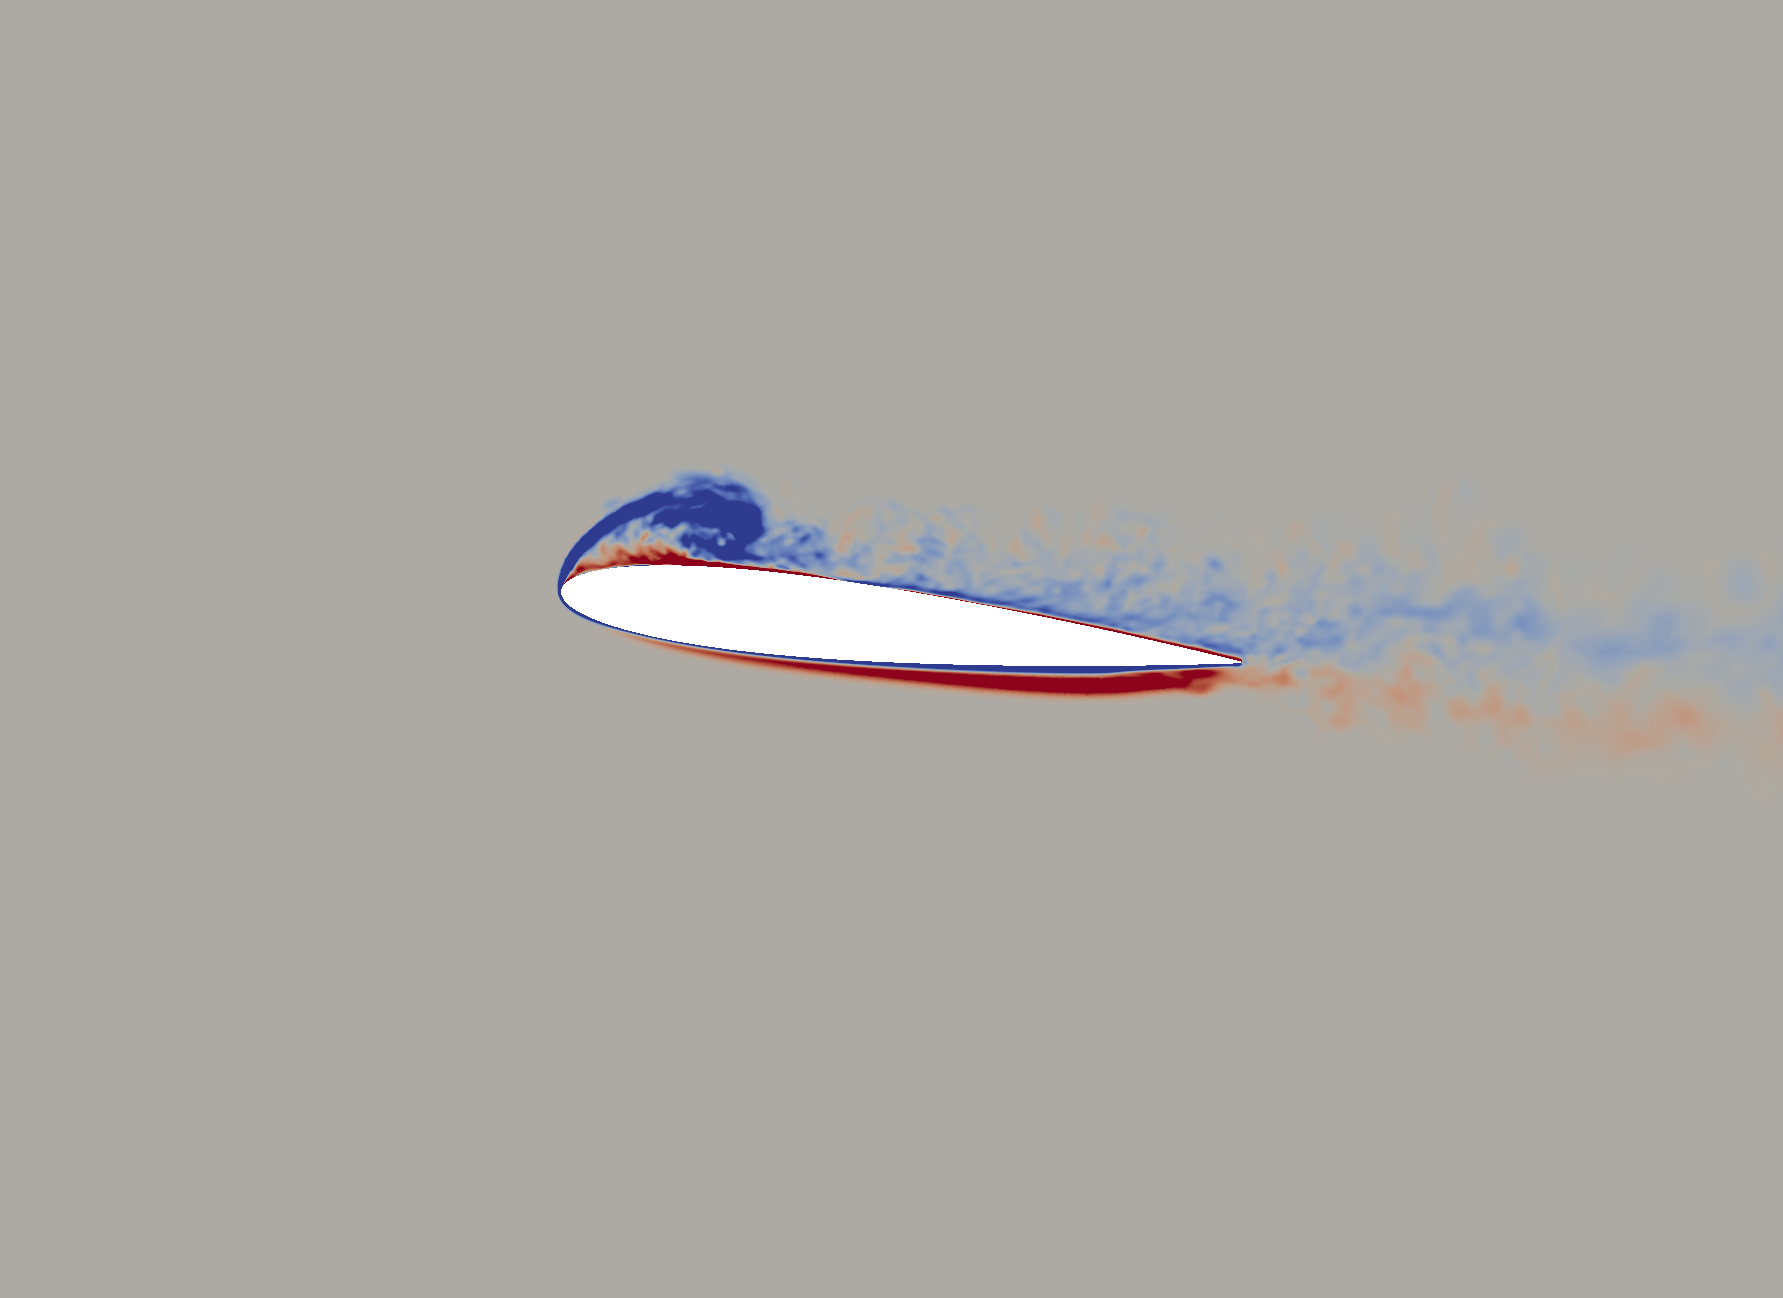
\includegraphics[width=1\textwidth]{figures/Vorticity_plots/Re_40k_1pt2/phase_225.png}
		\caption{$Re=4e4$, $\psi$ = $225^\circ$, $\tilde{t}=0.625$}
		\label{fig:Re_40k_1pt2_phi225}
	\end{subfigure}
	\begin{subfigure}[b]{0.32\textwidth}
		\centering
		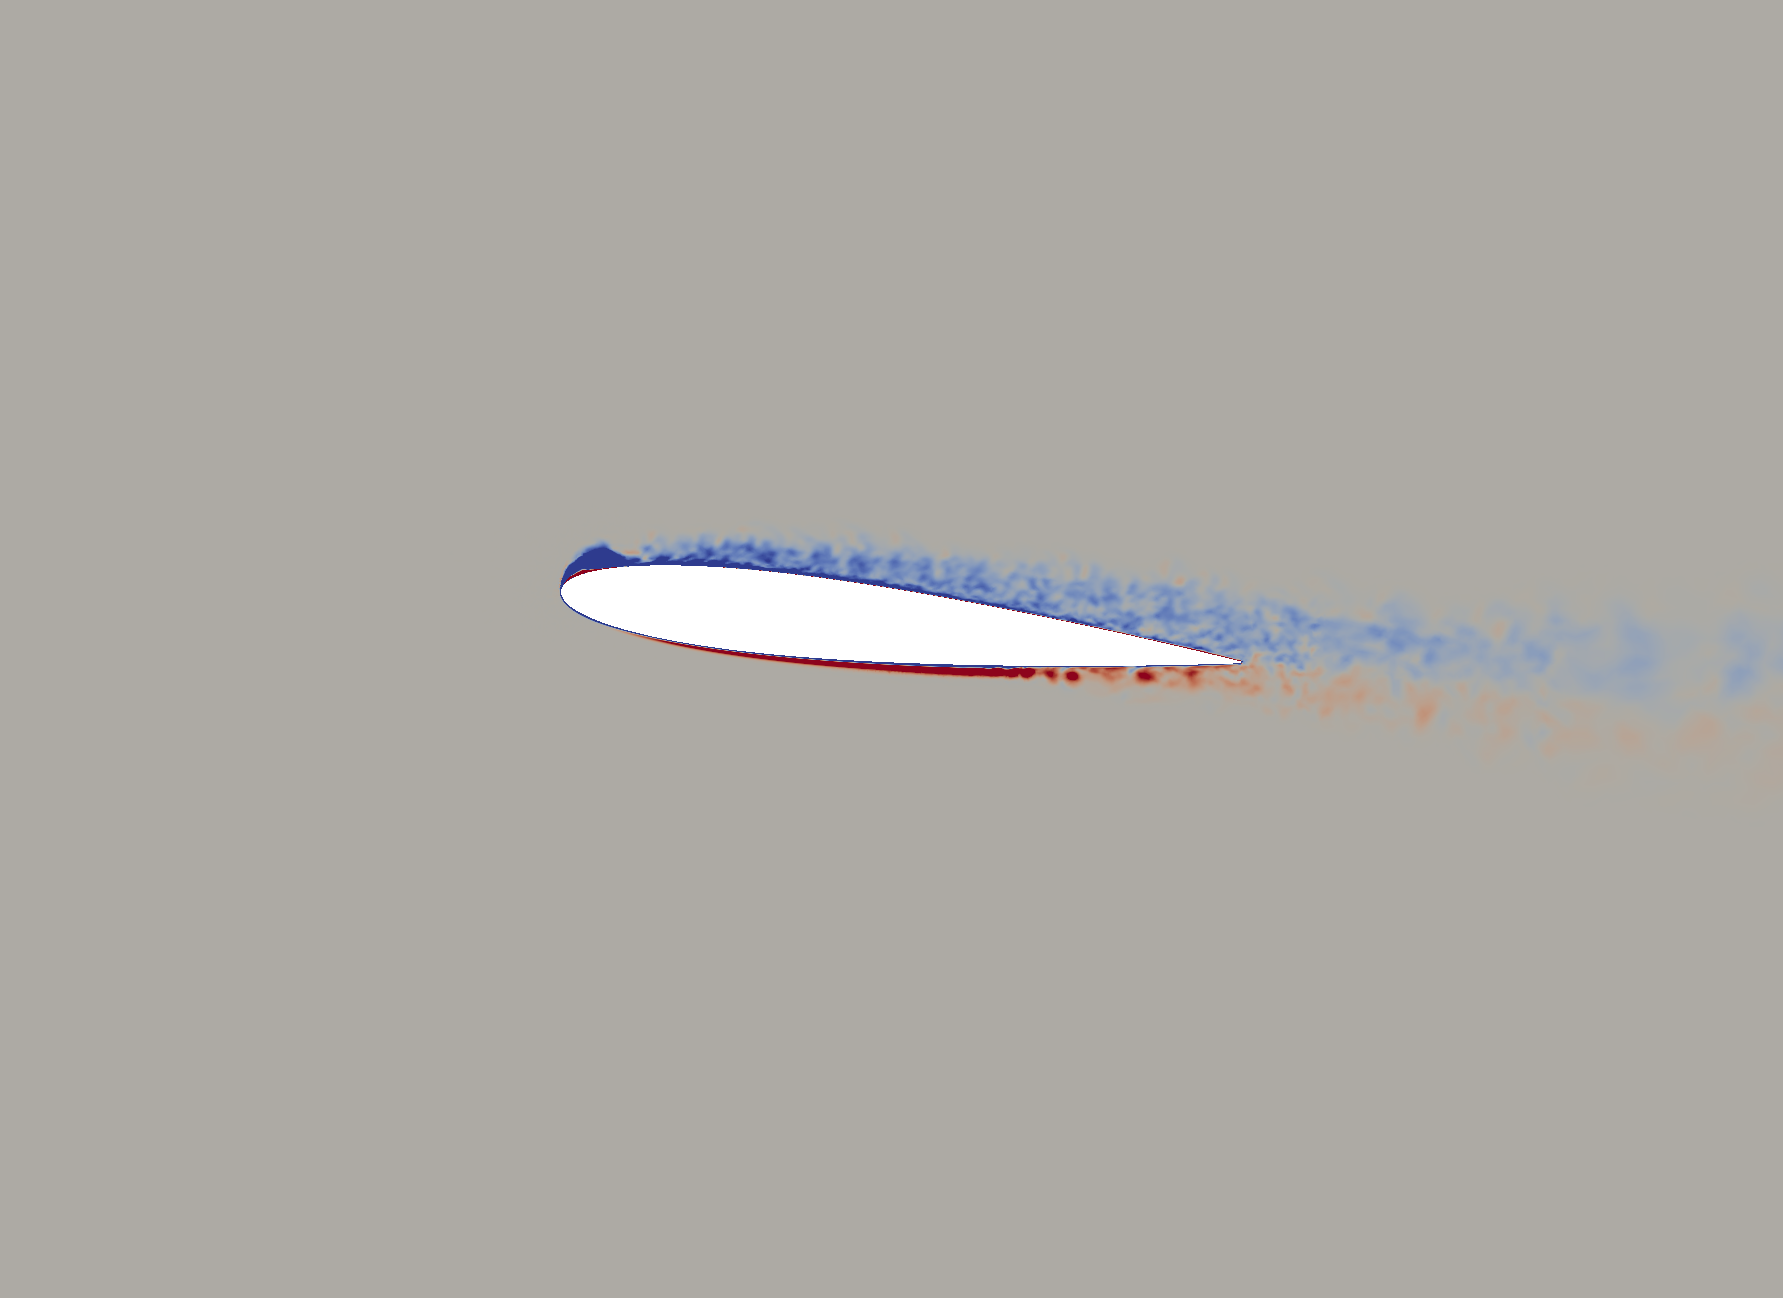
\includegraphics[width=1\textwidth]{figures/Vorticity_plots/Re_200k_1pt2/phase_225.png}
		\caption{$Re=2e5$, $\psi$ = $225^\circ$, $\tilde{t}=0.625$}
		\label{fig:Re_200k_1pt2_phi225}
	\end{subfigure}
	\begin{subfigure}[b]{0.32\textwidth}
		\centering
		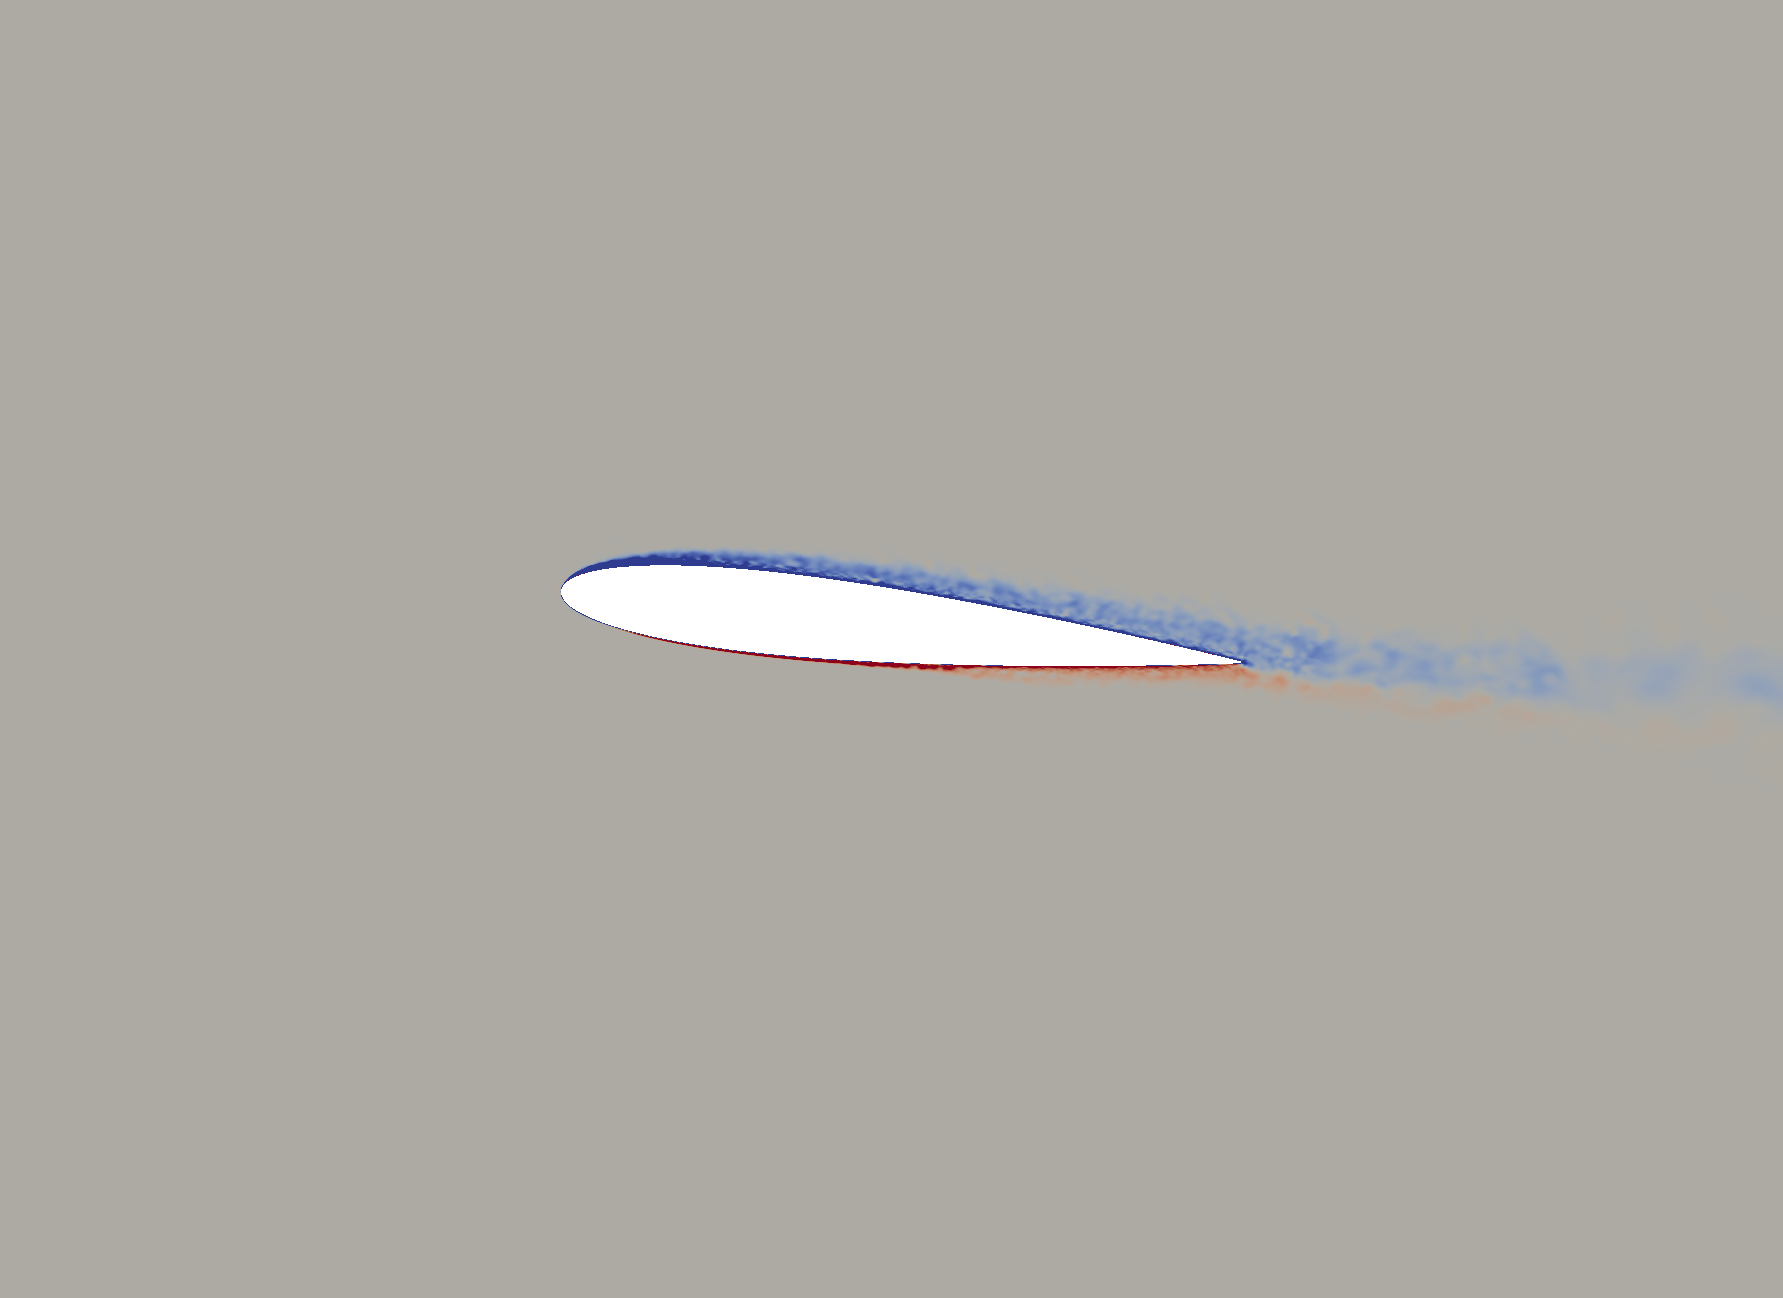
\includegraphics[width=1\textwidth]{figures/Vorticity_plots/Re_1m_1pt2/phase_225.png}
		\caption{$Re=1e6$, $\psi$ = $225^\circ$, $\tilde{t}=0.625$}
		\label{fig:Re_1m_1pt2_phi225}
	\end{subfigure}
	
	\begin{subfigure}[b]{0.32\textwidth}
		\centering
		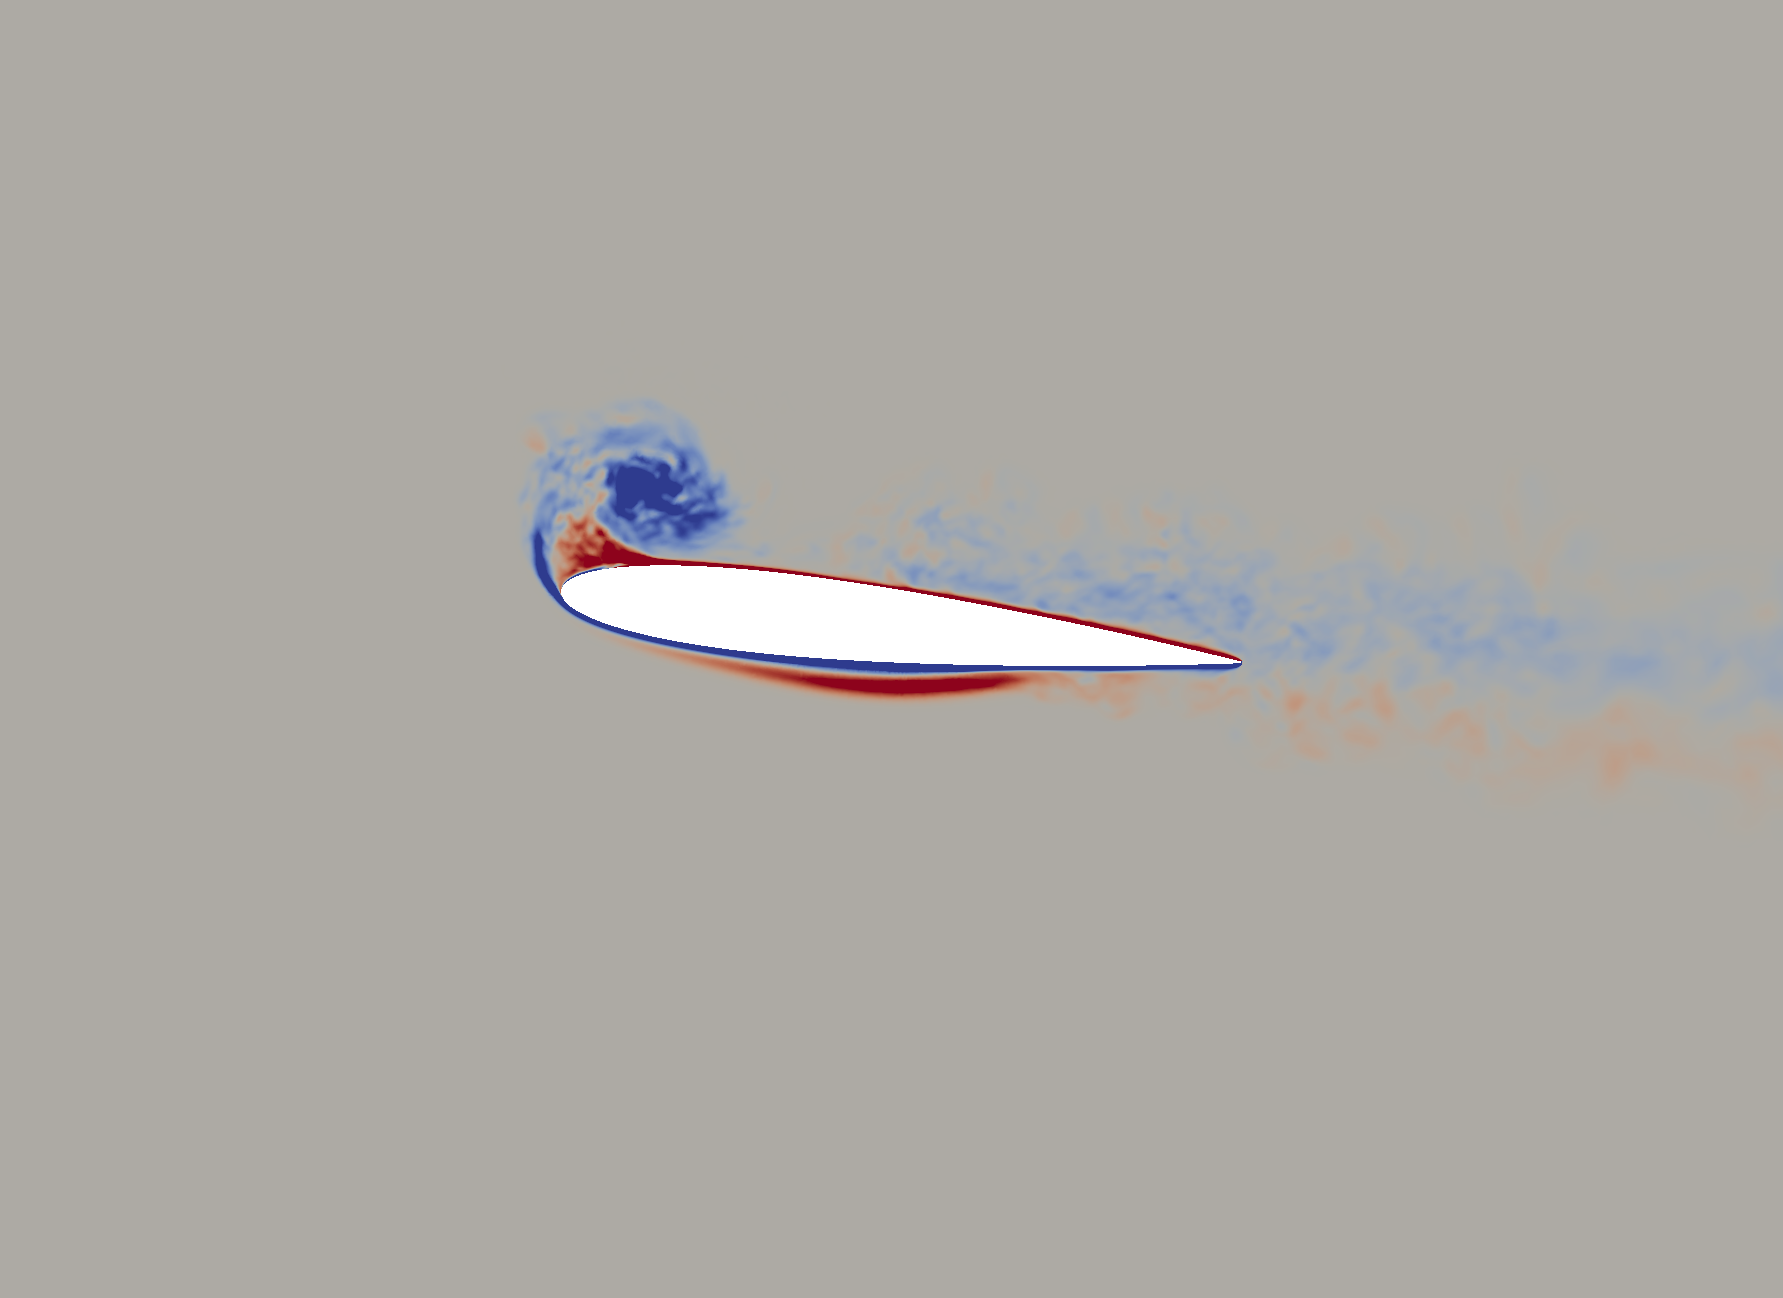
\includegraphics[width=1\textwidth]{figures/Vorticity_plots/Re_40k_1pt2/phase_240.png}
		\caption{$Re=4e4$, $\psi$ = $240^\circ$, $\tilde{t}=0.667$}
		\label{fig:Re_40k_1pt2_phi240}
	\end{subfigure}
	\begin{subfigure}[b]{0.32\textwidth}
		\centering
		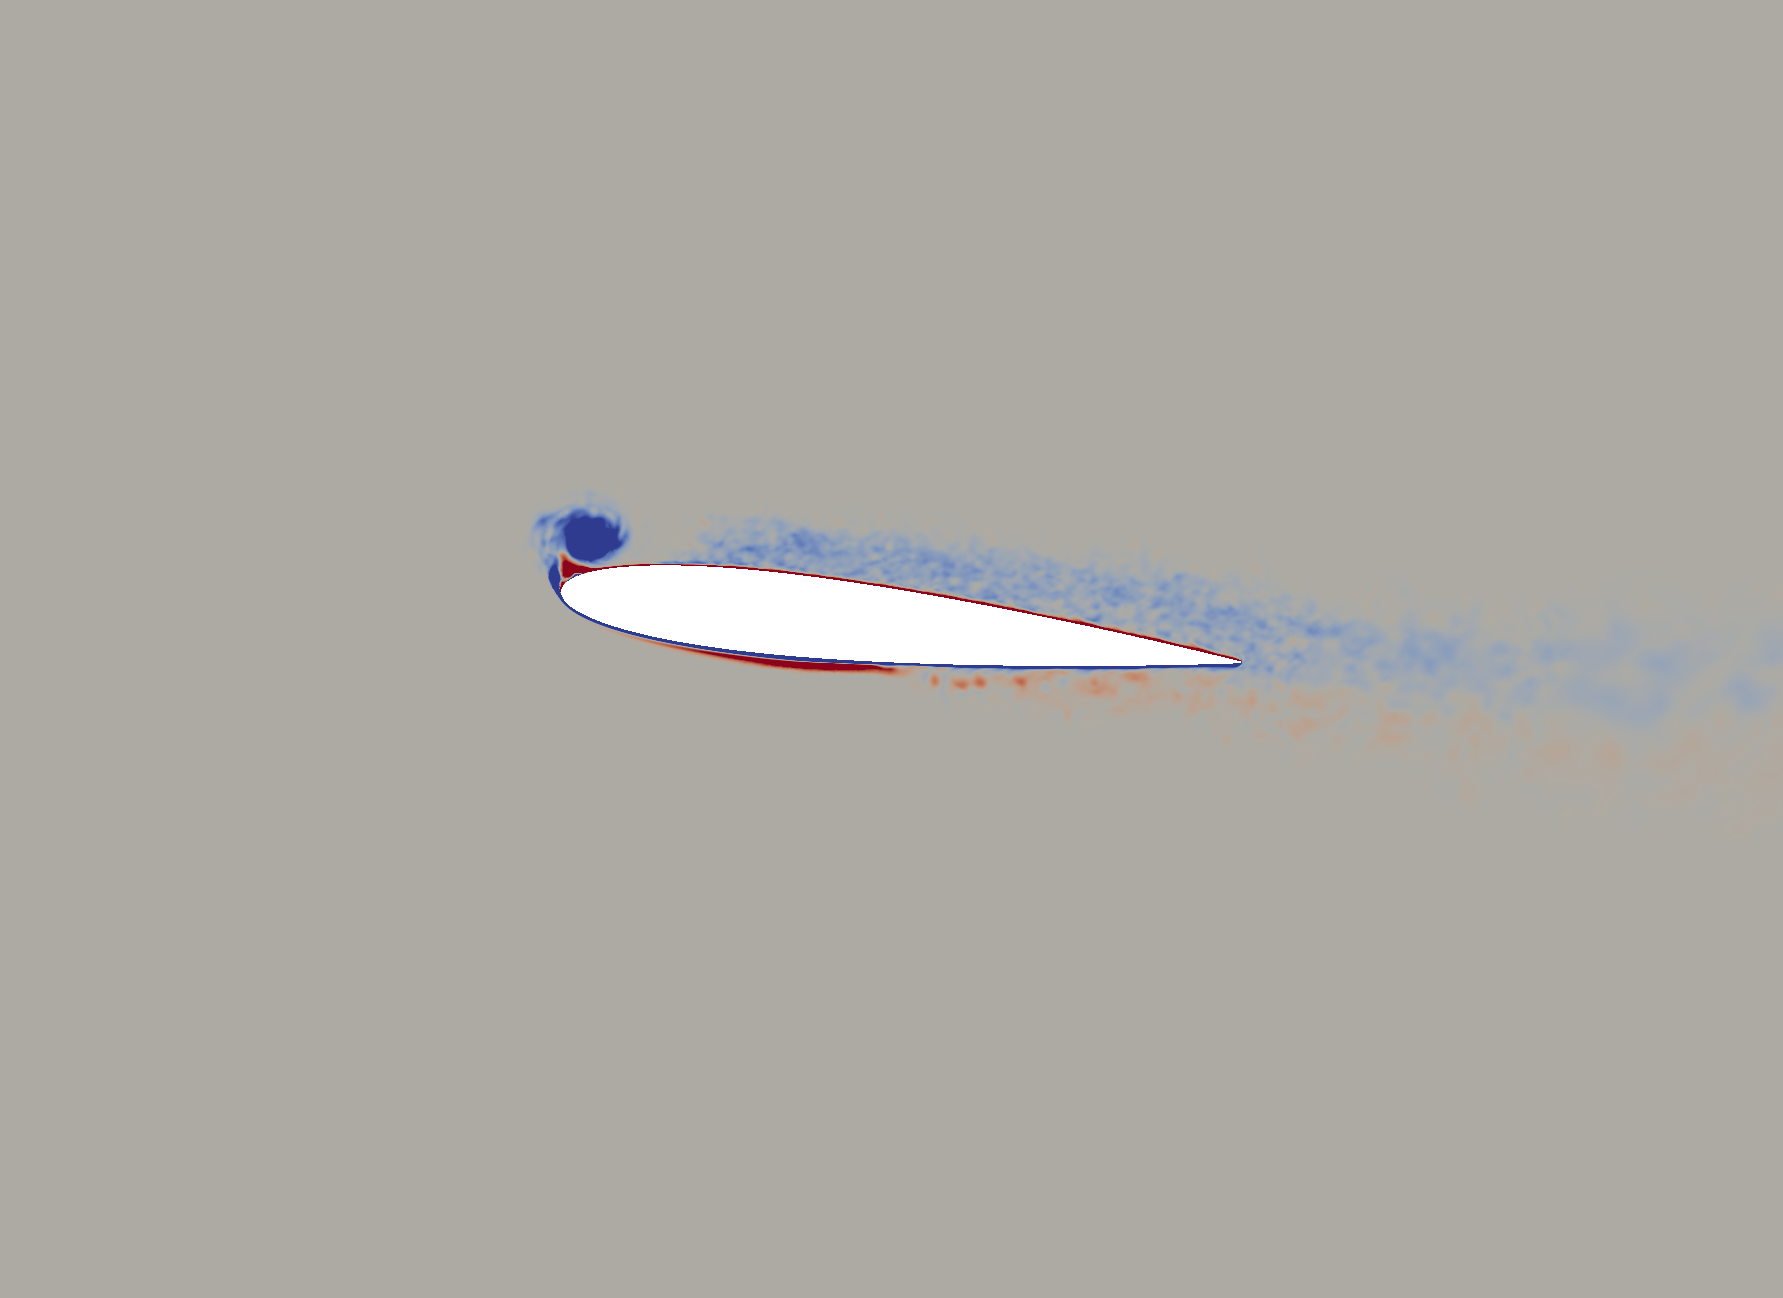
\includegraphics[width=1\textwidth]{figures/Vorticity_plots/Re_200k_1pt2/phase_240.png}
		\caption{$Re=2e5$, $\psi$ = $240^\circ$, $\tilde{t}=0.667$}
		\label{fig:Re_200k_1pt2_phi240}
	\end{subfigure}
	\begin{subfigure}[b]{0.32\textwidth}
		\centering
		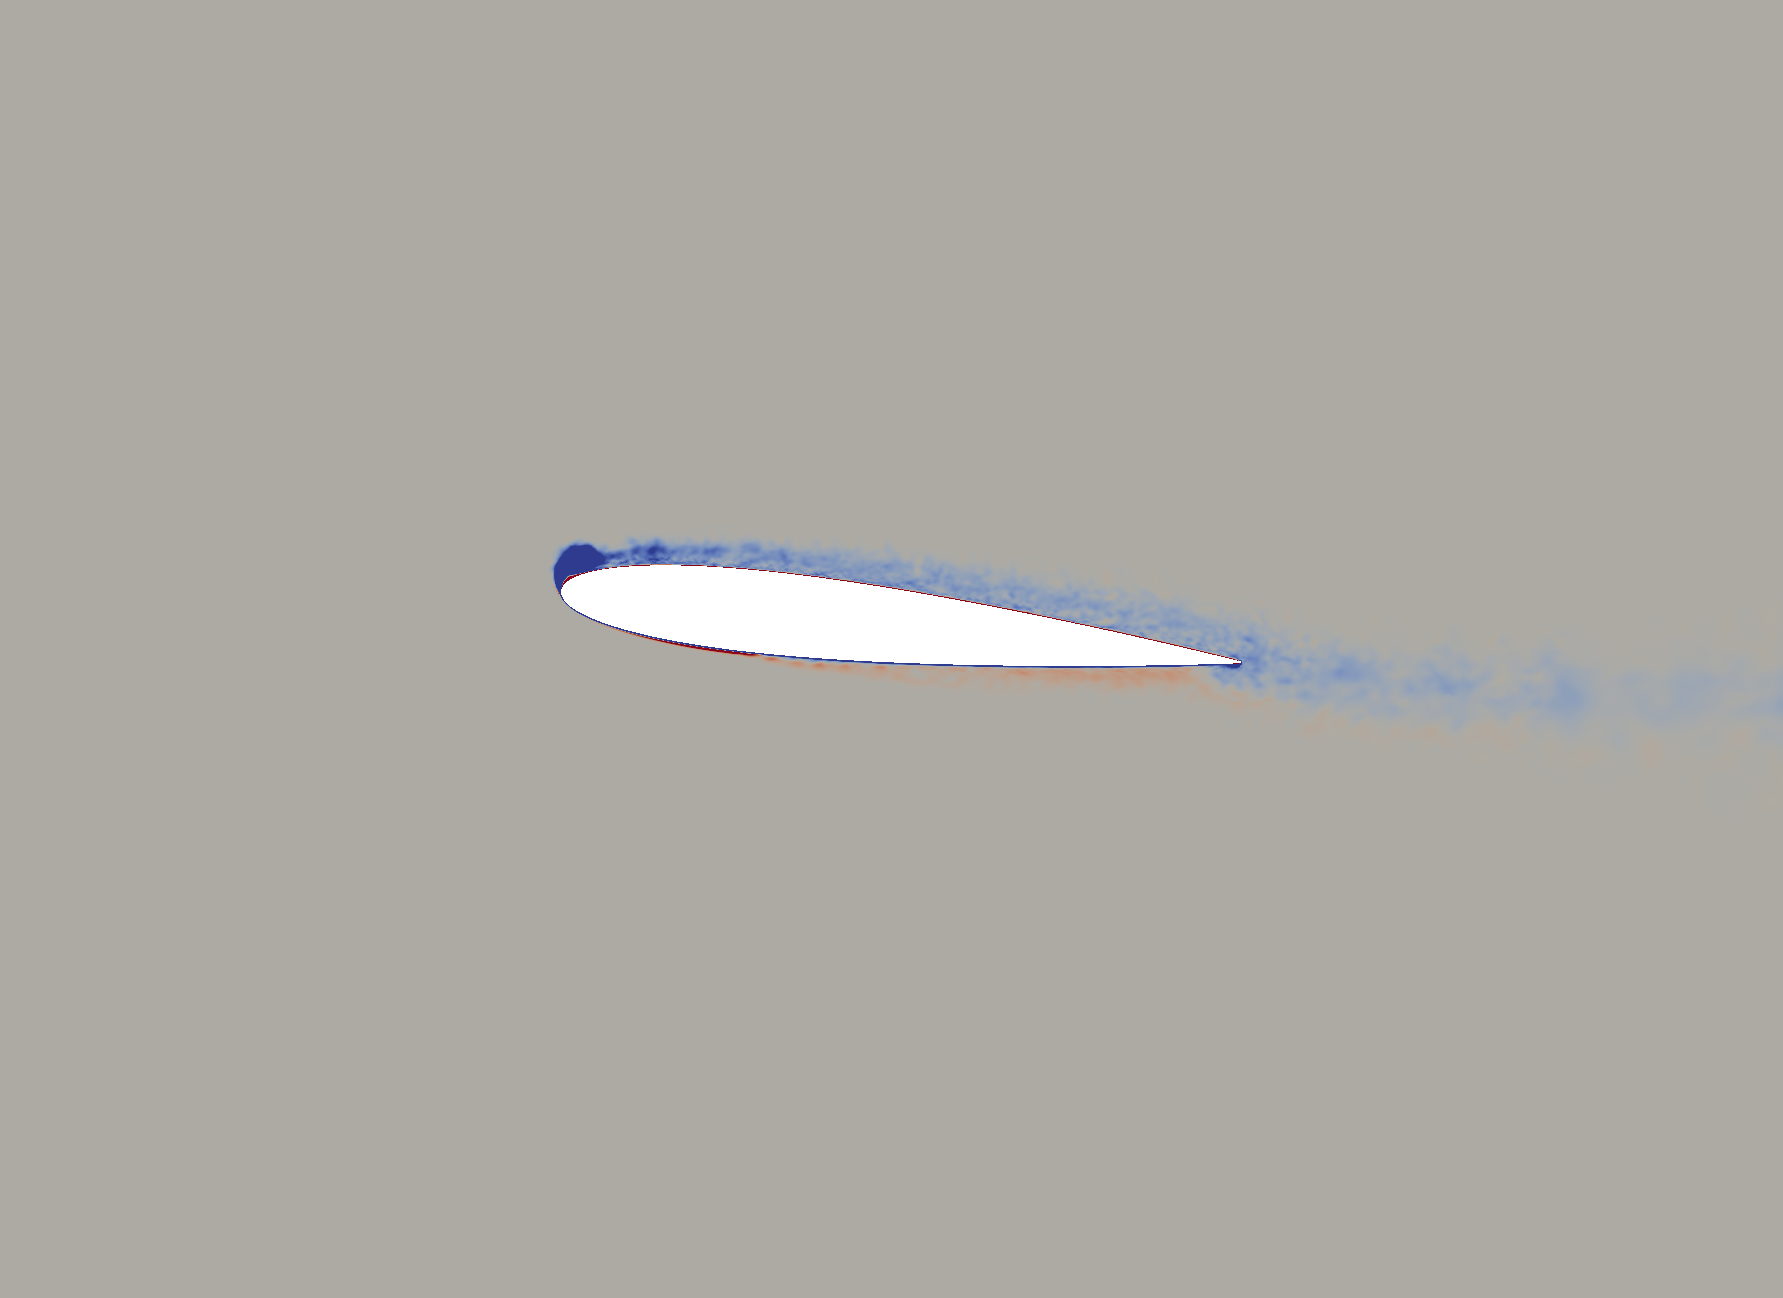
\includegraphics[width=1\textwidth]{figures/Vorticity_plots/Re_1m_1pt2/phase_240.png}
		\caption{$Re=1e6$, $\psi$ = $240^\circ$, $\tilde{t}=0.667$}
		\label{fig:Re_1m_1pt2_phi240}
	\end{subfigure}
	
	\begin{subfigure}[b]{0.32\textwidth}
		\centering
		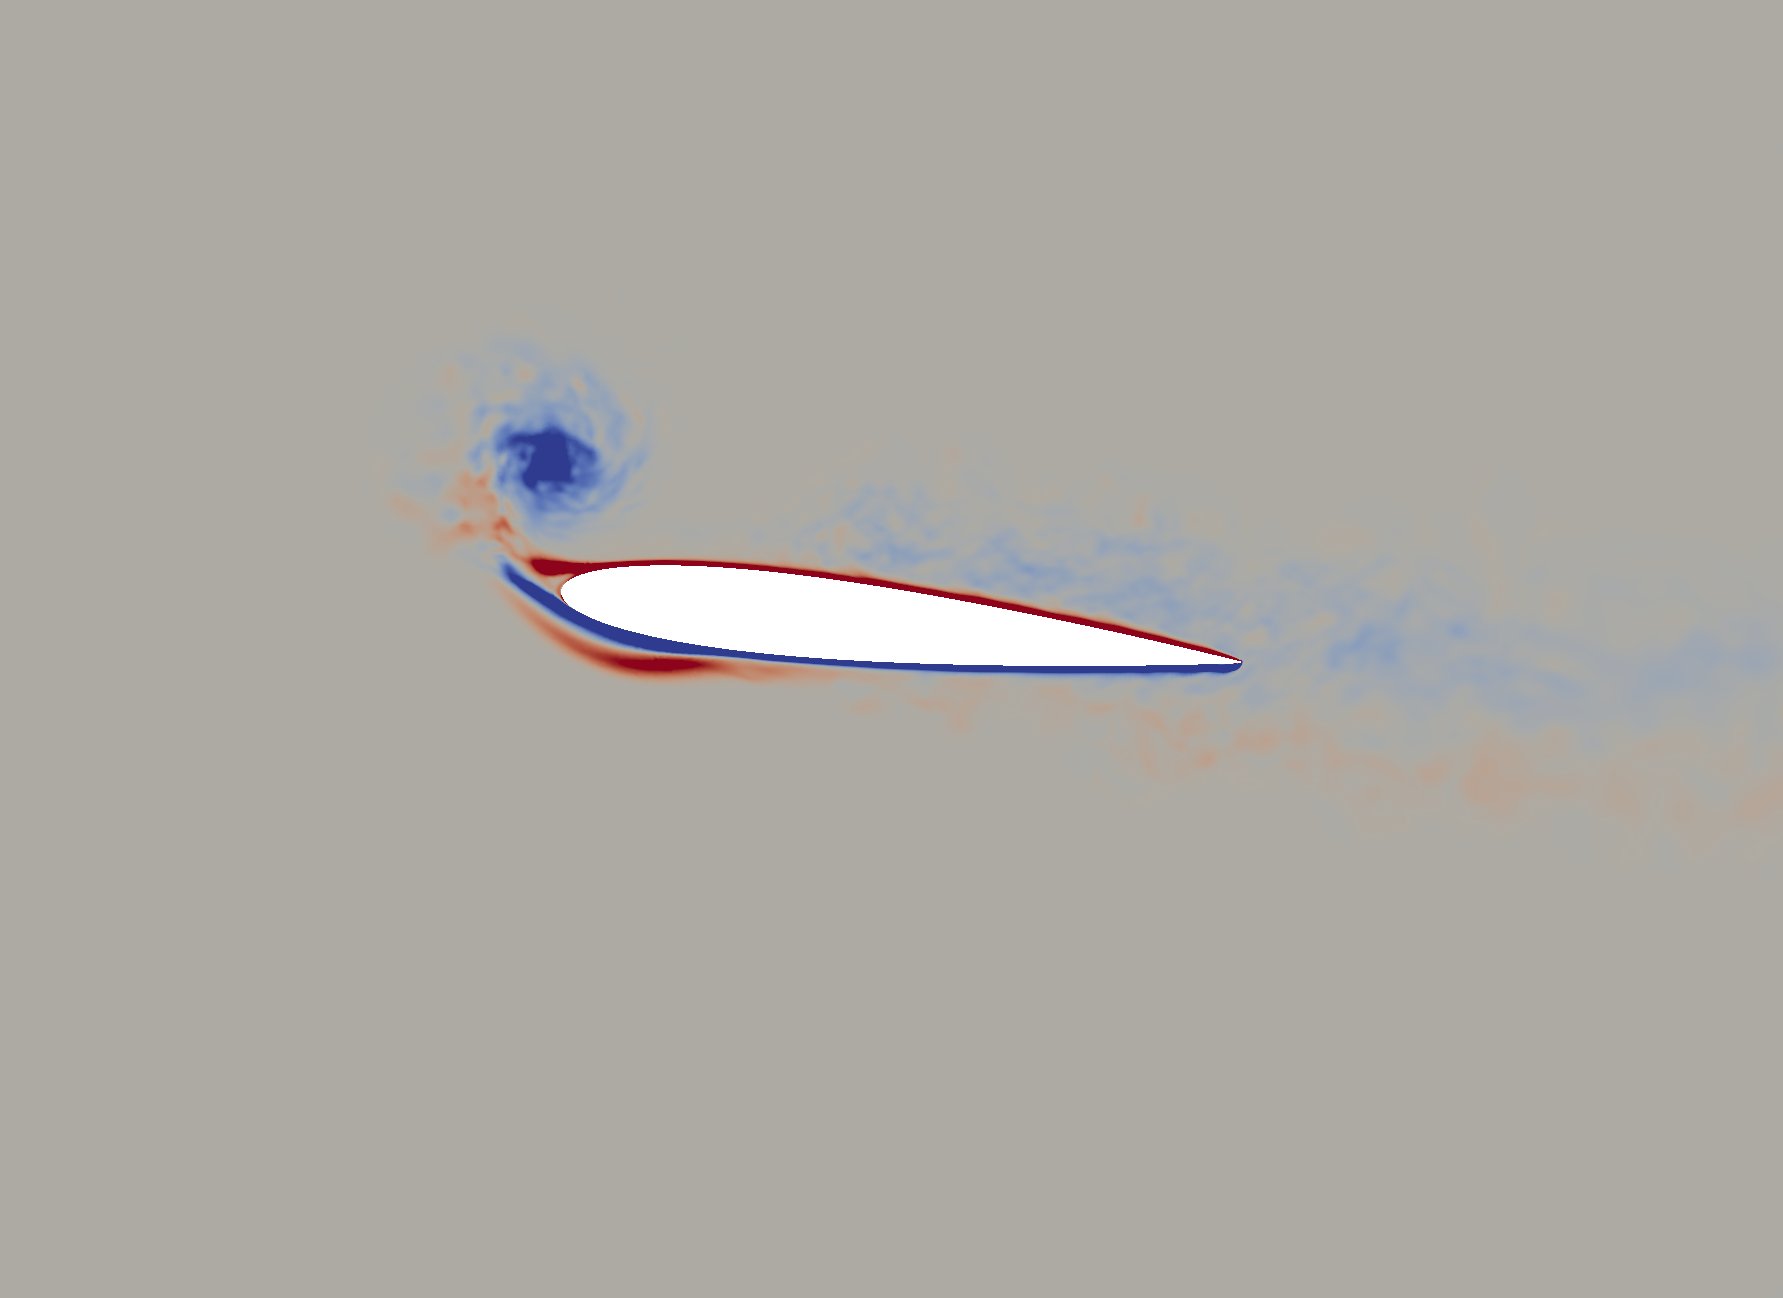
\includegraphics[width=1\textwidth]{figures/Vorticity_plots/Re_40k_1pt2/phase_255.png}
		\caption{$Re=4e4$, $\psi$ = $255^\circ$, $\tilde{t}=0.708$}
		\label{fig:Re_40k_1pt2_phi255}
	\end{subfigure}
	\begin{subfigure}[b]{0.32\textwidth}
		\centering
		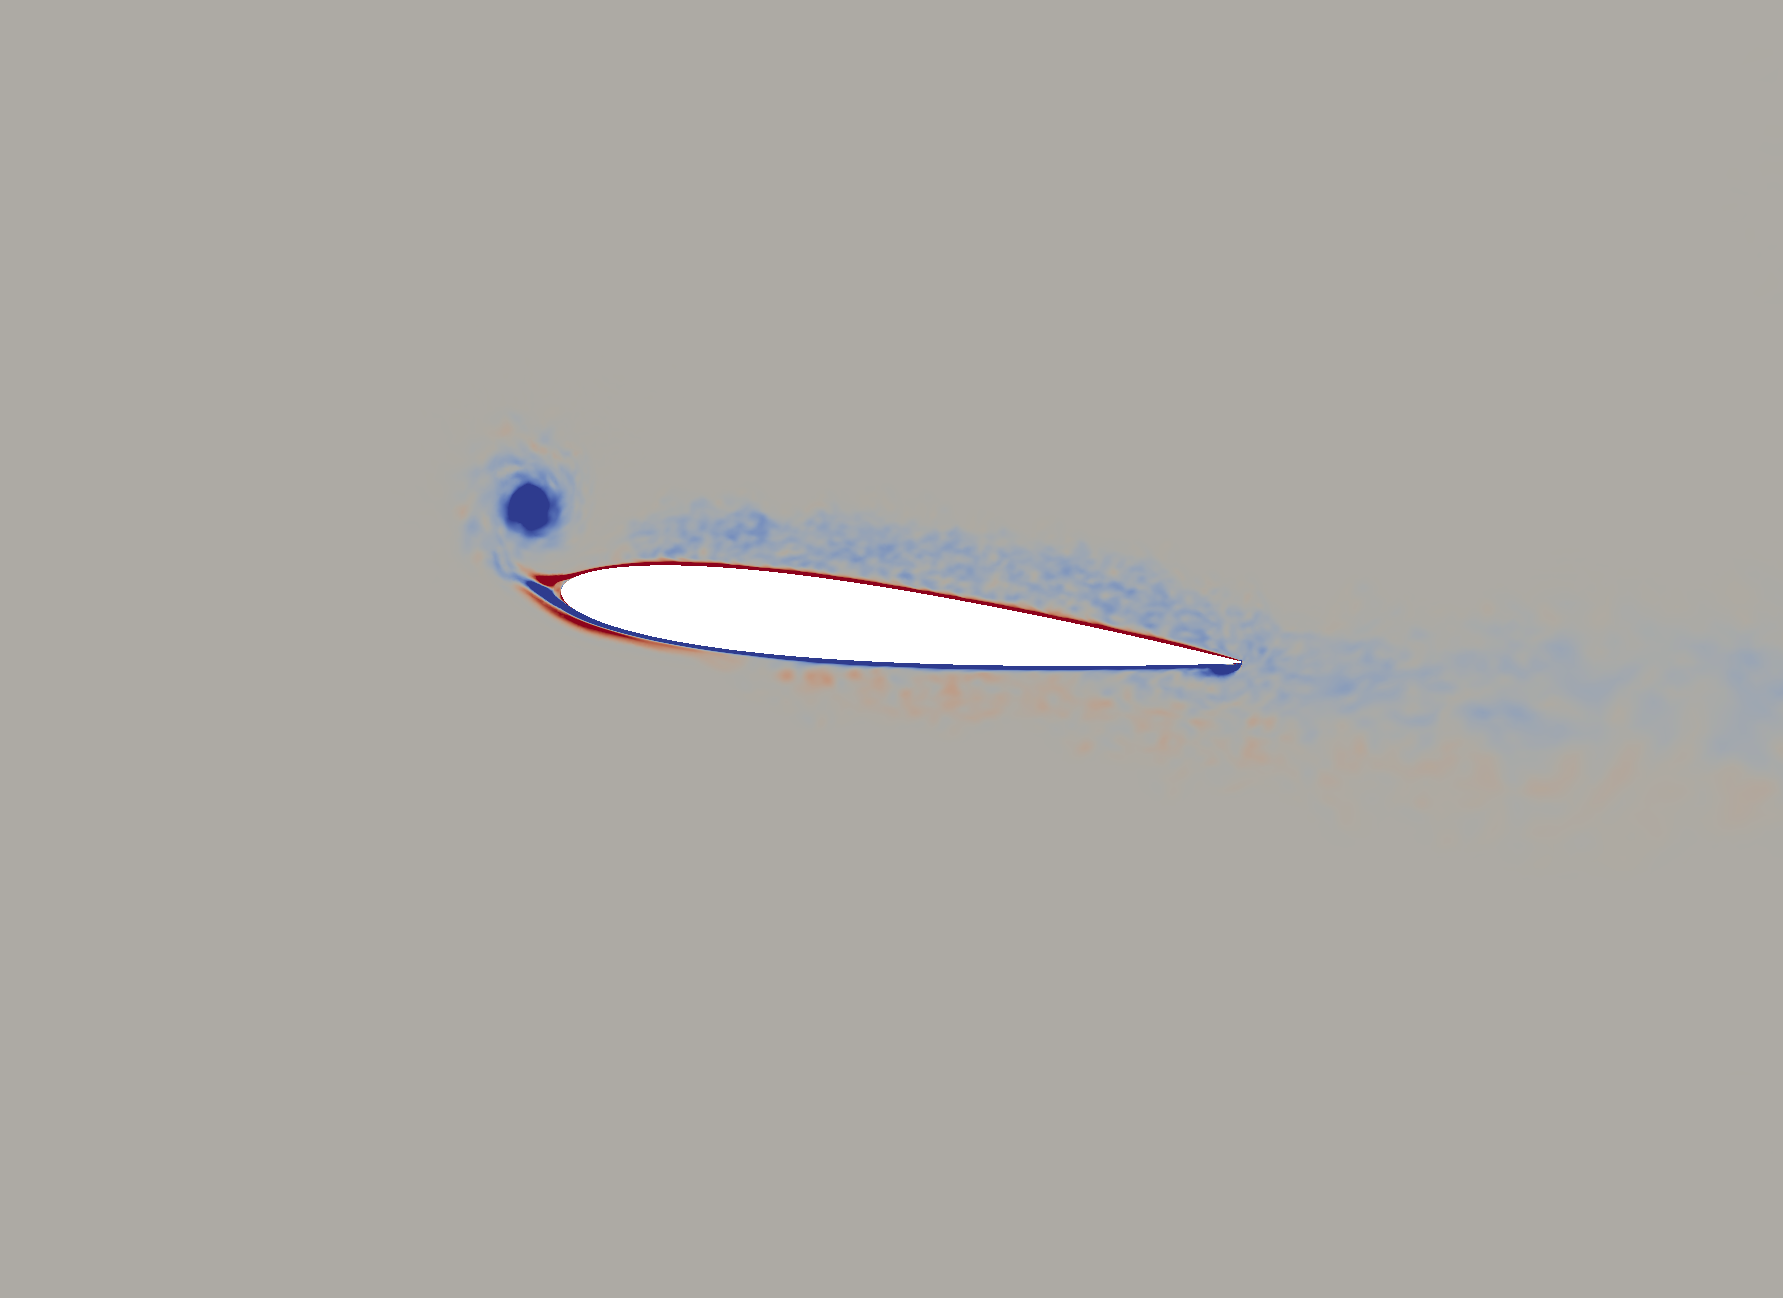
\includegraphics[width=1\textwidth]{figures/Vorticity_plots/Re_200k_1pt2/phase_255.png}
		\caption{$Re=2e5$, $\psi$ = $255^\circ$, $\tilde{t}=0.708$}
		\label{fig:Re_200k_1pt2_phi255}
	\end{subfigure}
	\begin{subfigure}[b]{0.32\textwidth}
		\centering
		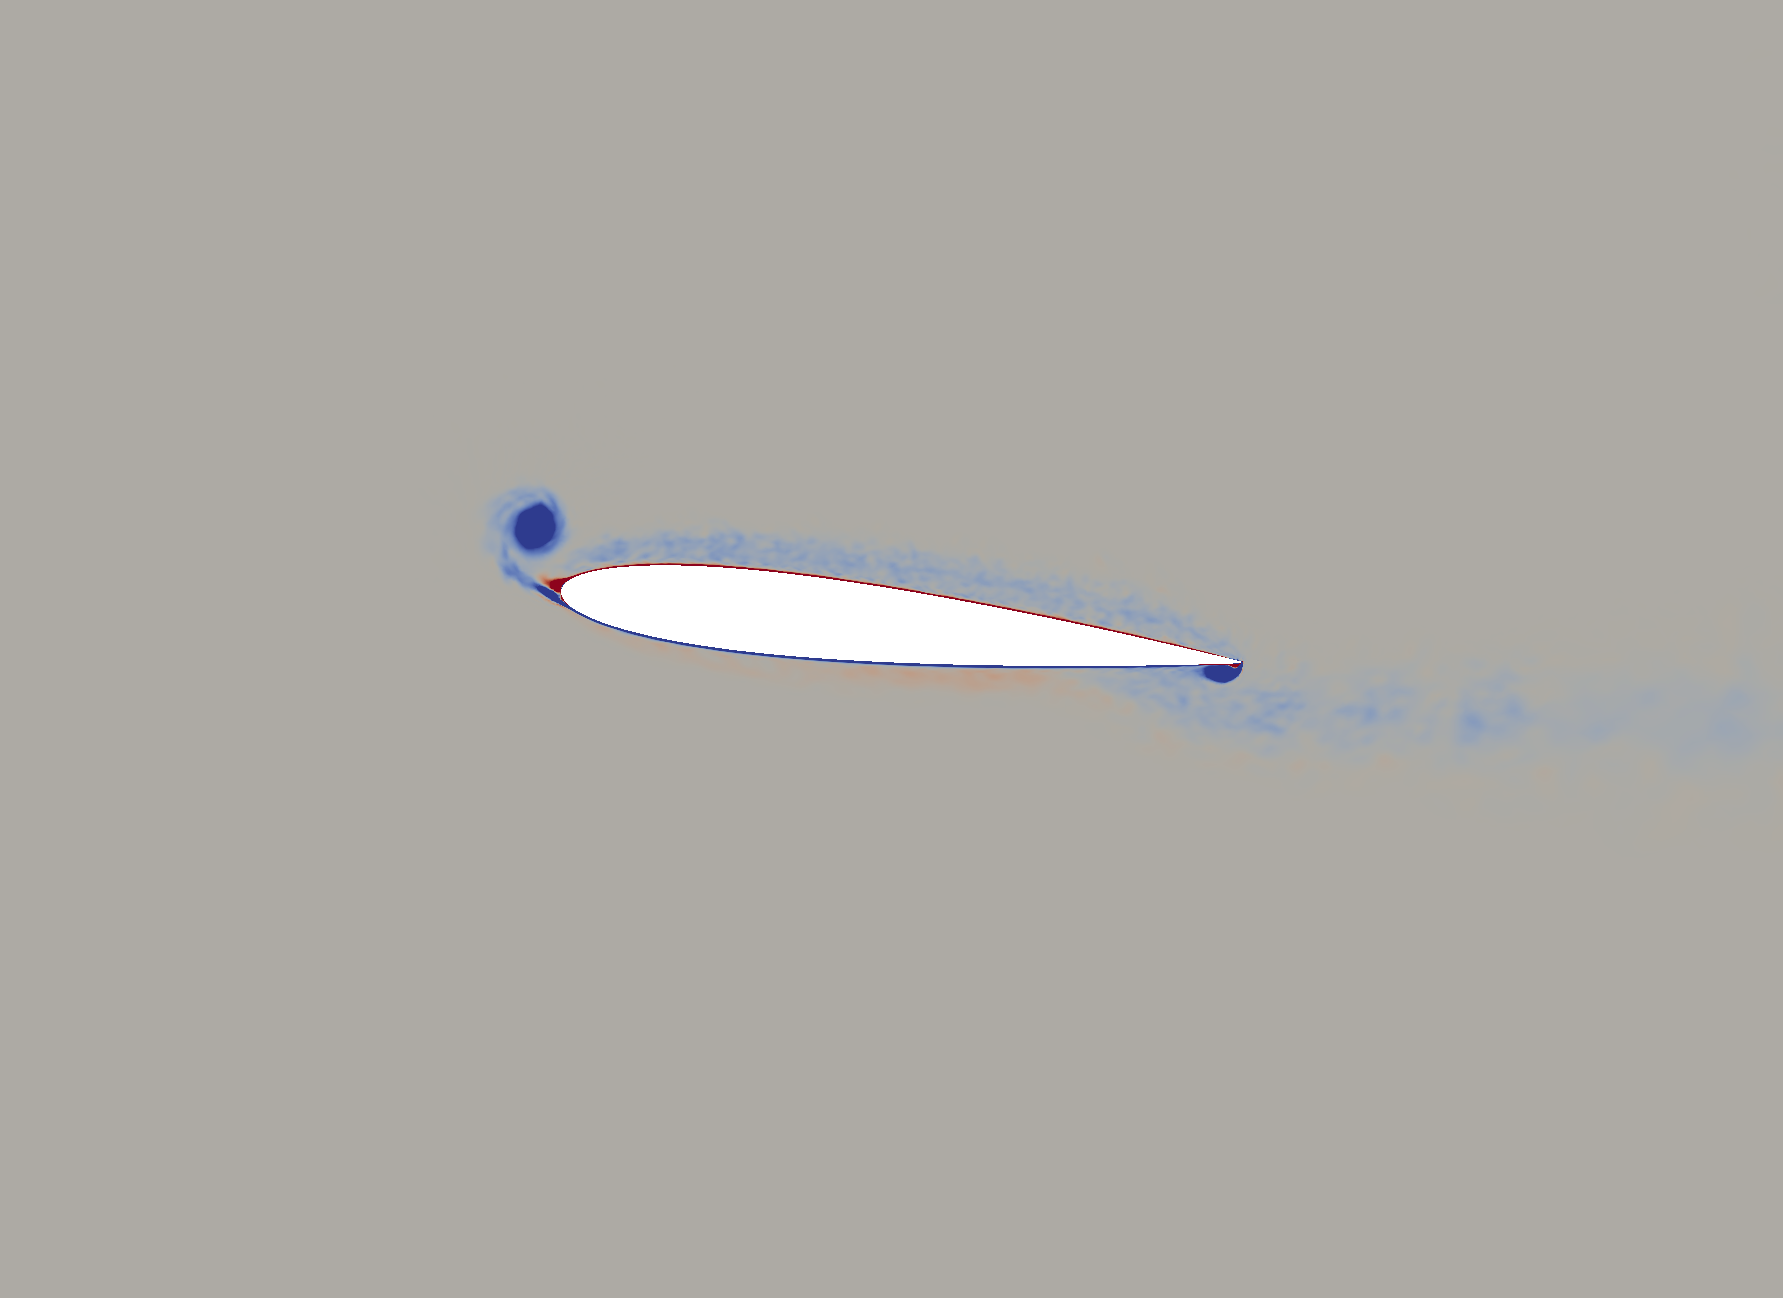
\includegraphics[width=1\textwidth]{figures/Vorticity_plots/Re_1m_1pt2/phase_255.png}
		\caption{$Re=1e6$, $\psi$ = $255^\circ$, $\tilde{t}=0.708$}
		\label{fig:Re_1m_1pt2_phi255}
	\end{subfigure}
	
	\caption{Spanwise vorticity at 8 different phases for $Re$=40,000 (left column), 200,000 (middle column) and 1,000,000 (right column) at $\lambda$ = 1.2}
%	\label{fig:vortScreen_1pt2}
\end{figure}


\begin{figure}[H]\ContinuedFloat
	\centering
	\begin{subfigure}[b]{0.32\textwidth}
		\centering
		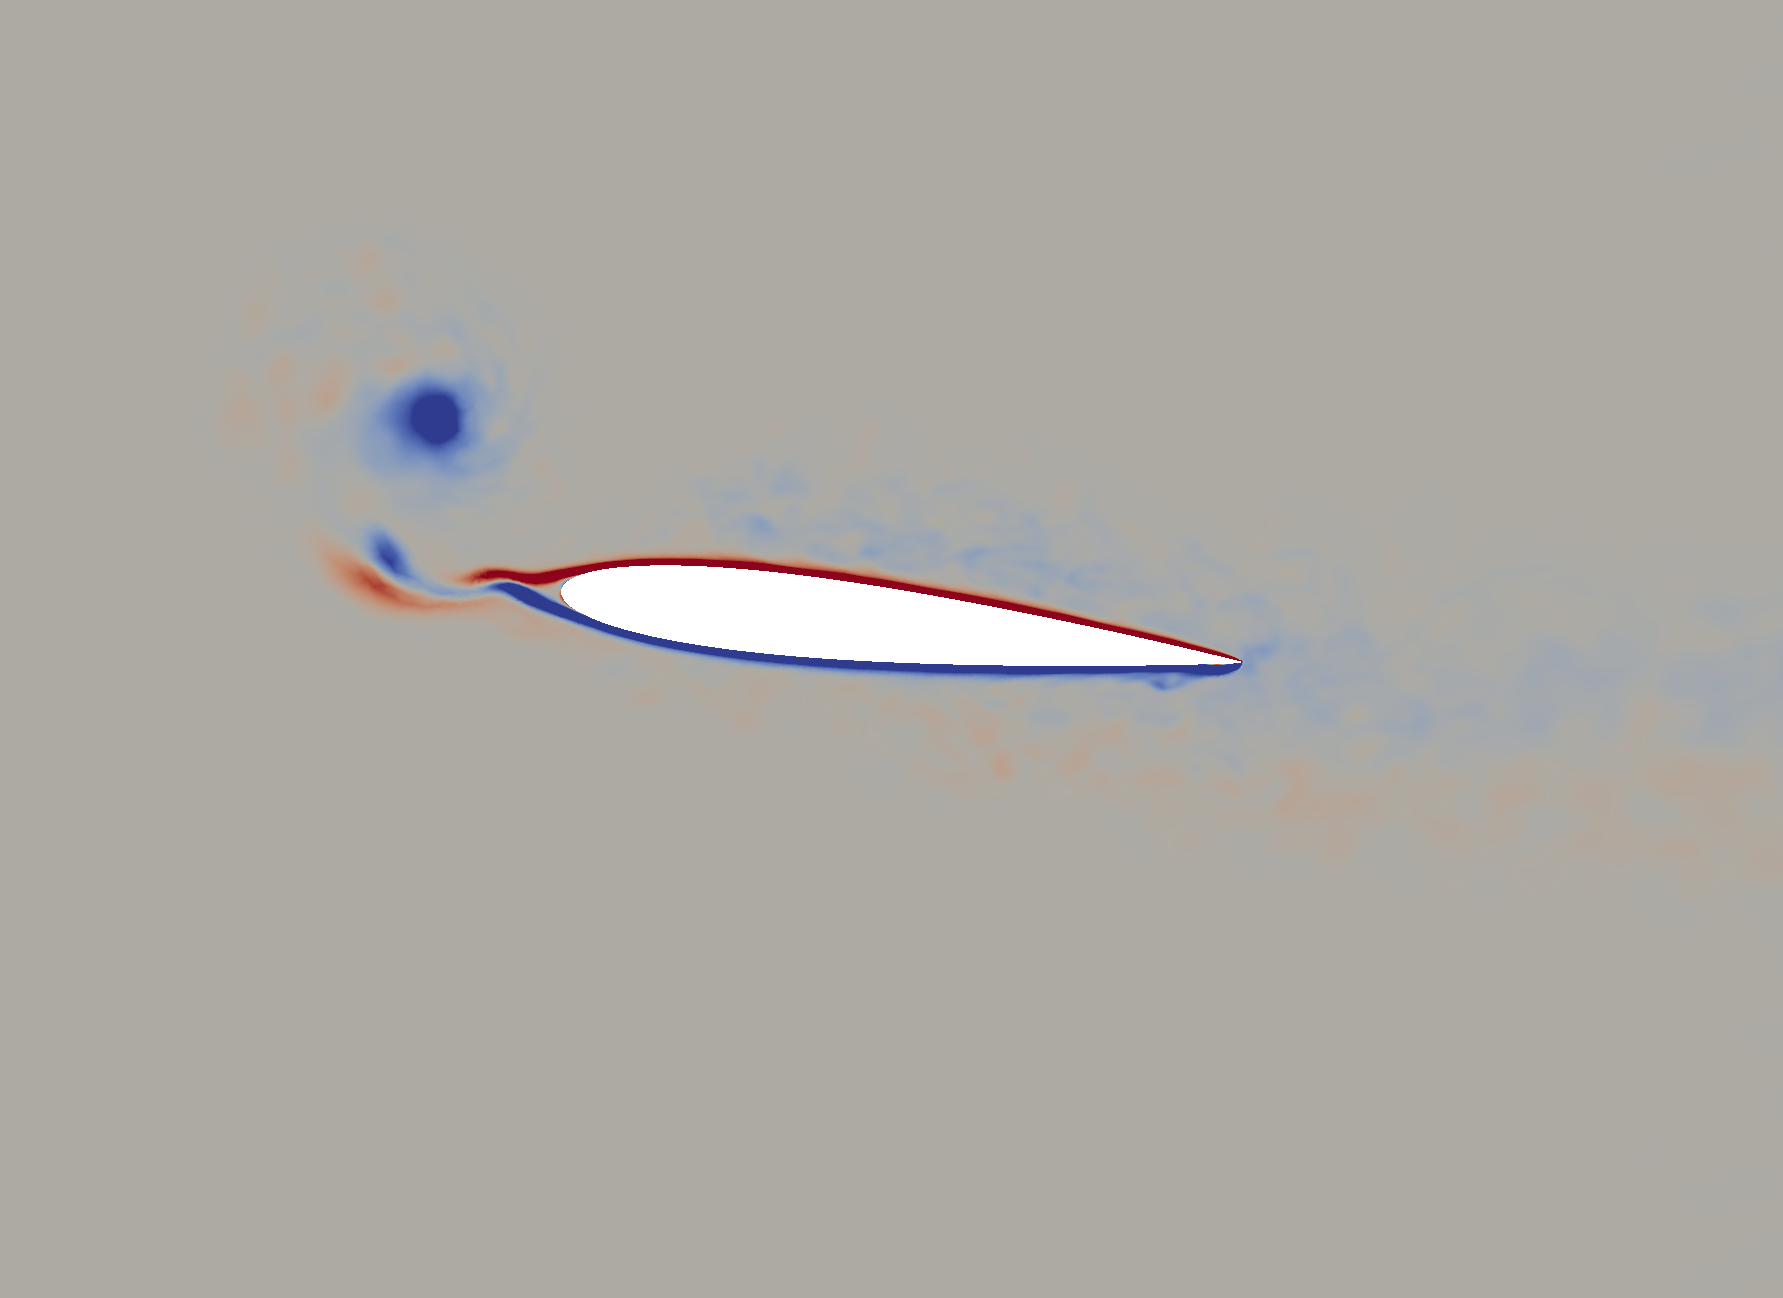
\includegraphics[width=1\textwidth]{figures/Vorticity_plots/Re_40k_1pt2/phase_270.png}
		\caption{$Re=4e4$, $\psi$ = $270^\circ$, $\tilde{t}=0.750$}
		\label{fig:Re_40k_1pt2_phi270}
	\end{subfigure}
	\begin{subfigure}[b]{0.32\textwidth}
		\centering
		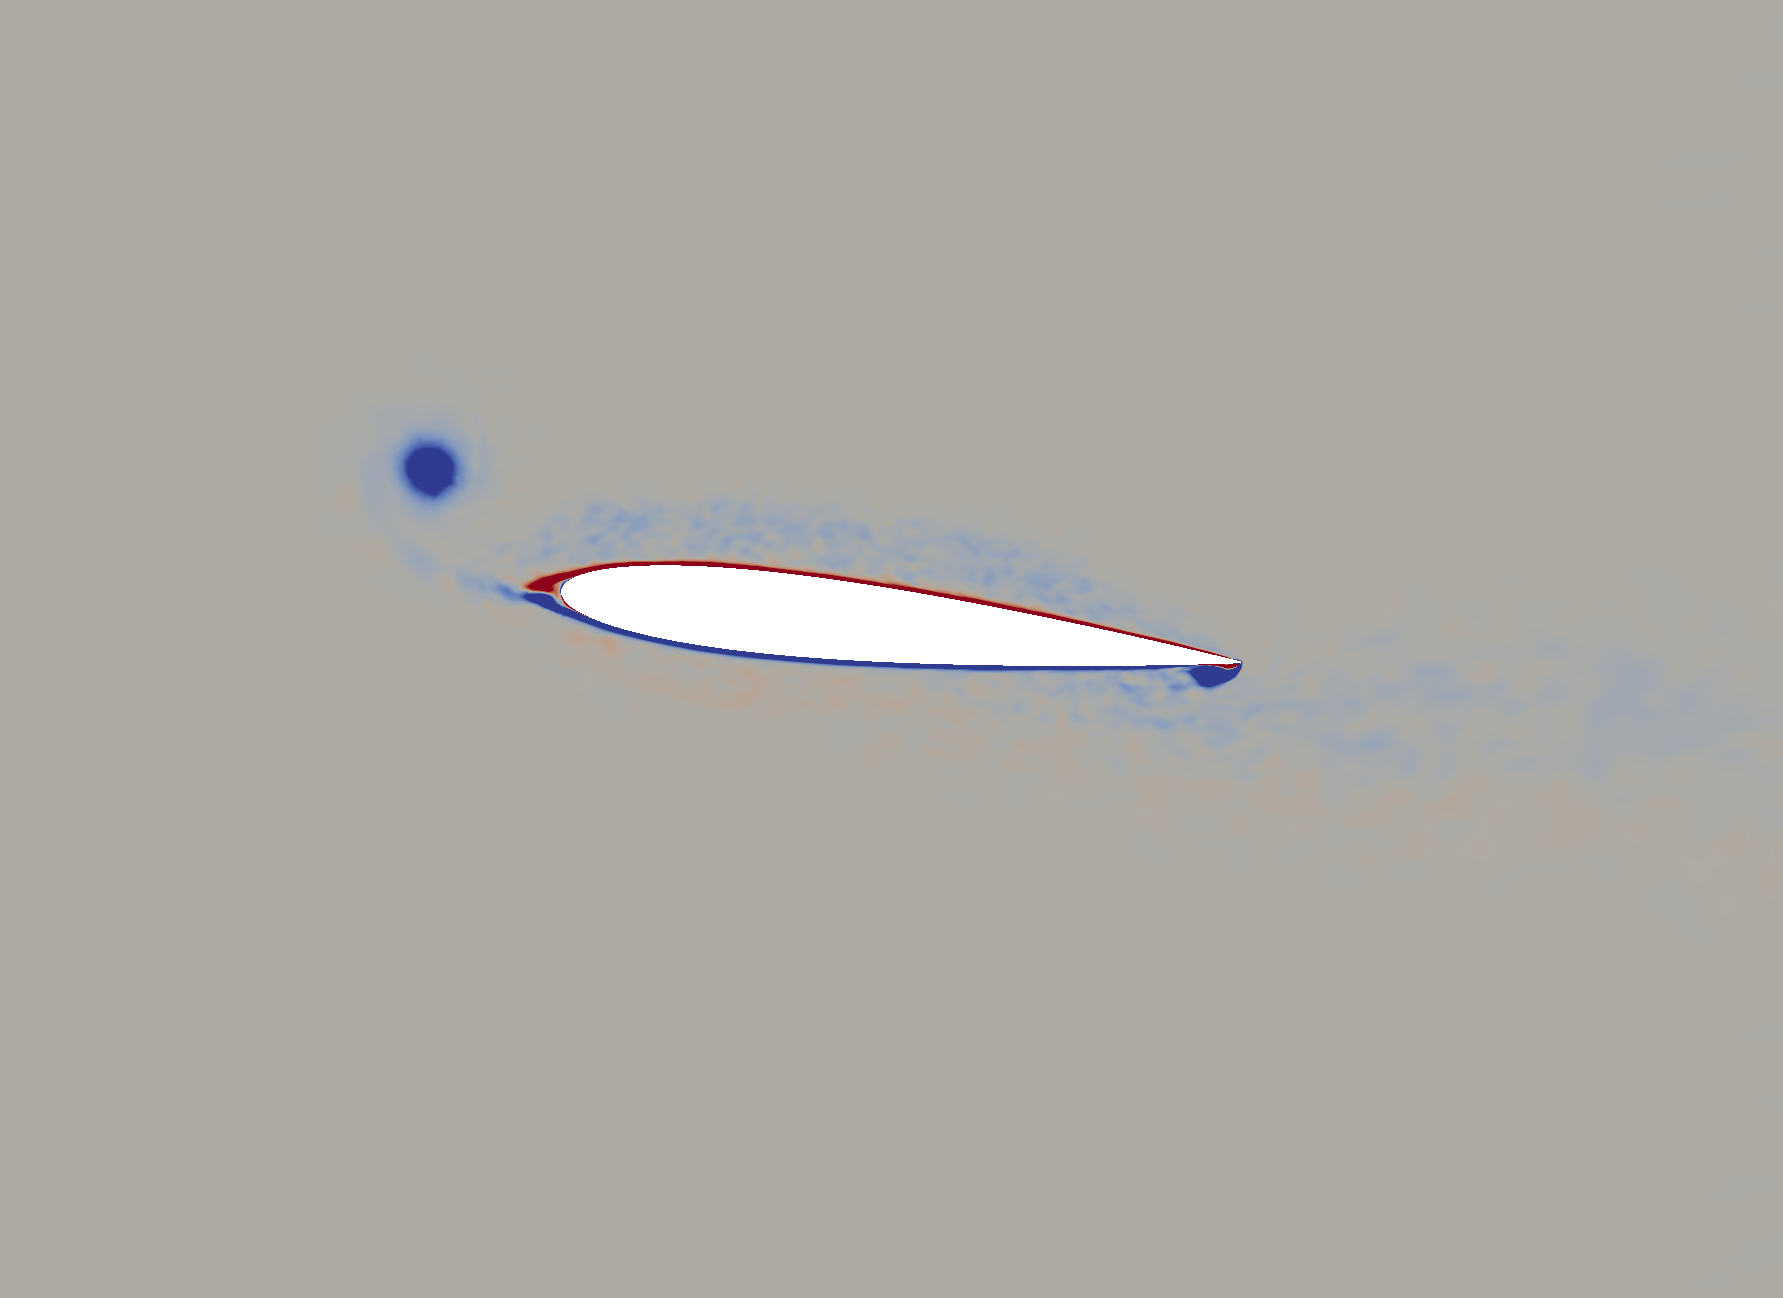
\includegraphics[width=1\textwidth]{figures/Vorticity_plots/Re_200k_1pt2/phase_270.png}
		\caption{$Re=2e5$, $\psi$ = $270^\circ$, $\tilde{t}=0.750$}
		\label{fig:Re_200k_1pt2_phi270}
	\end{subfigure}
	\begin{subfigure}[b]{0.32\textwidth}
		\centering
		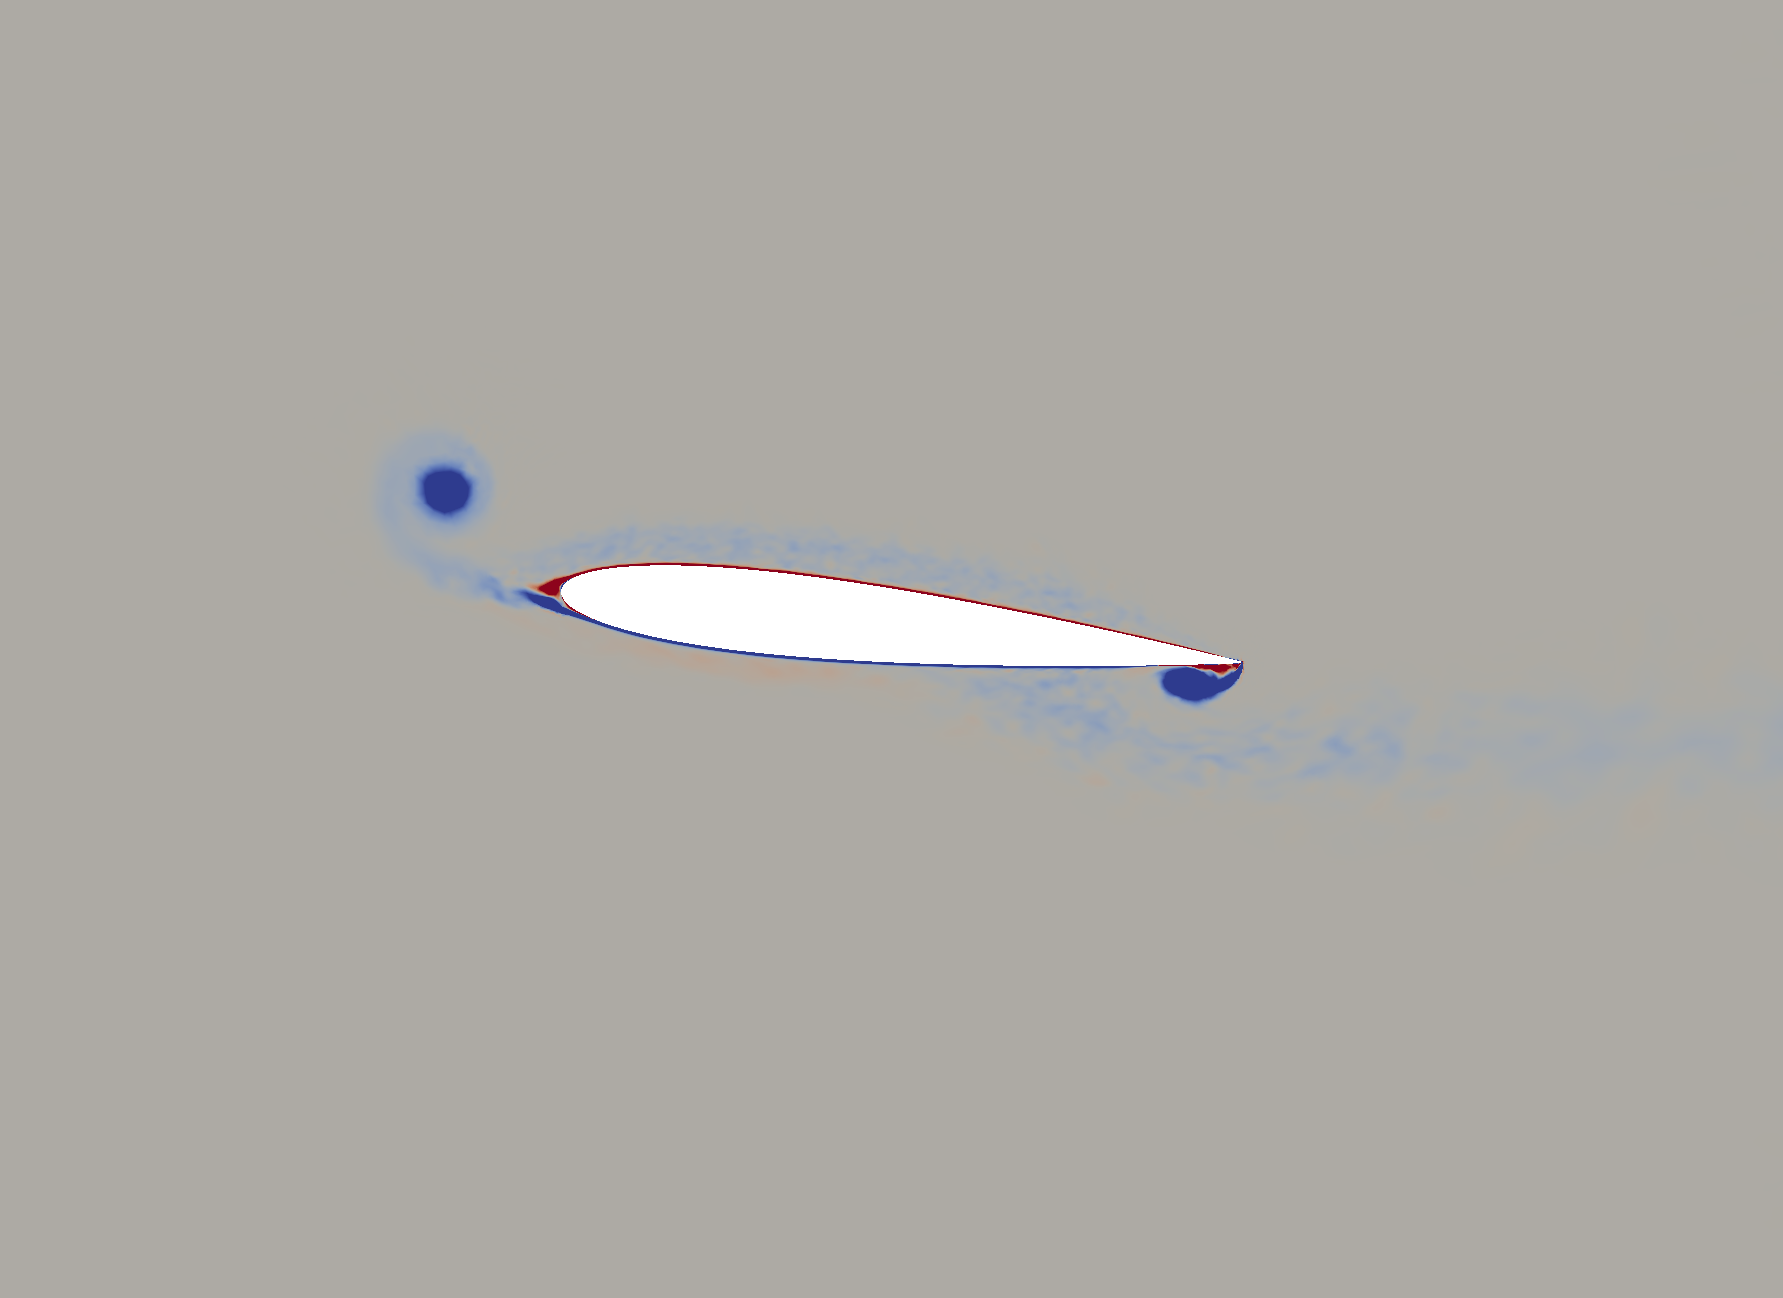
\includegraphics[width=1\textwidth]{figures/Vorticity_plots/Re_1m_1pt2/phase_270.png}
		\caption{$Re=1e6$, $\psi$ = $270^\circ$, $\tilde{t}=0.750$}
		\label{fig:Re_1m_1pt2_phi270}
	\end{subfigure}
	
	\begin{subfigure}[b]{0.32\textwidth}
		\centering
		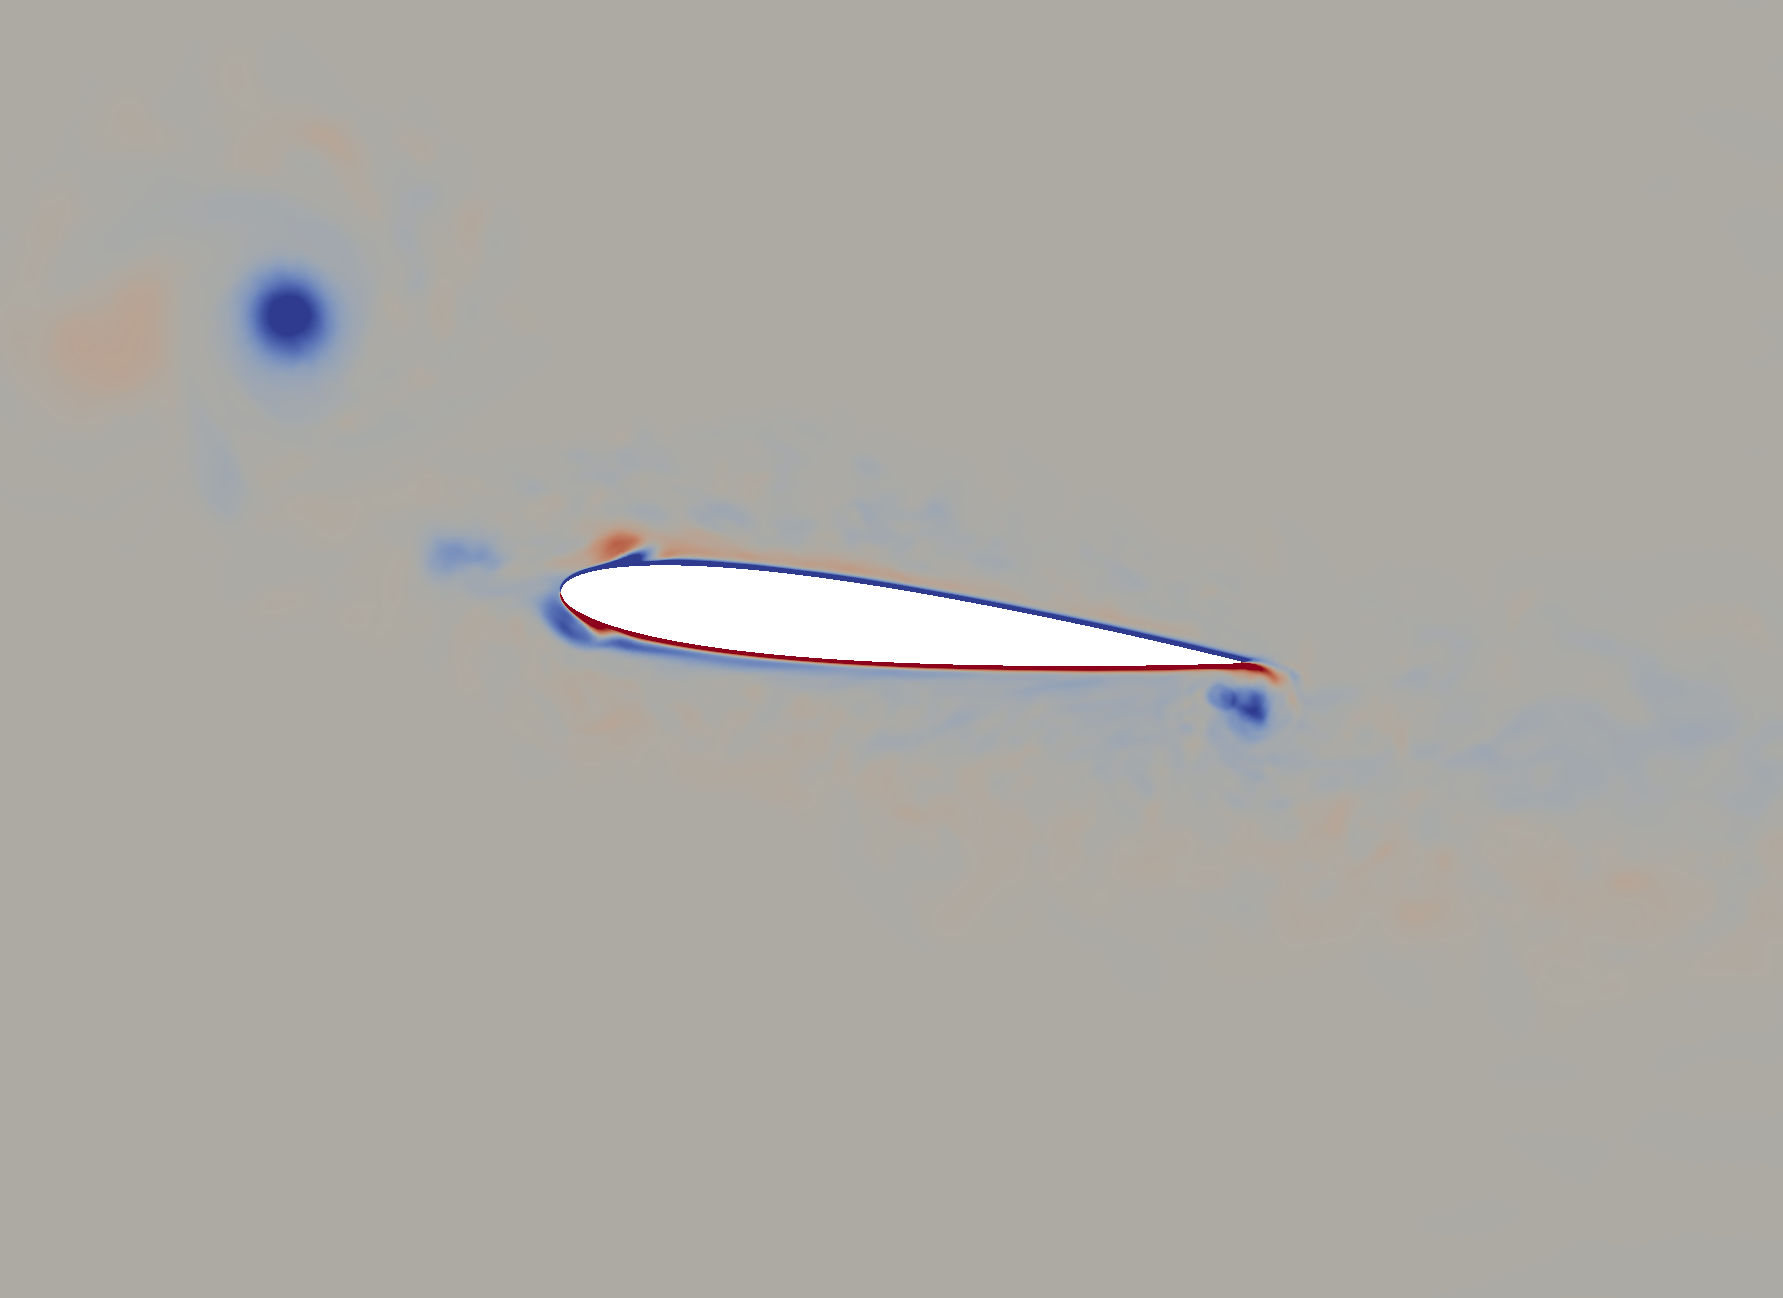
\includegraphics[width=1\textwidth]{figures/Vorticity_plots/Re_40k_1pt2/phase_315.png}
		\caption{$Re=4e4$, $\psi$ = $315^\circ$, $\tilde{t}=0.875$}
		\label{fig:Re_40k_1pt2_phi315}
	\end{subfigure}
	\begin{subfigure}[b]{0.32\textwidth}
		\centering
		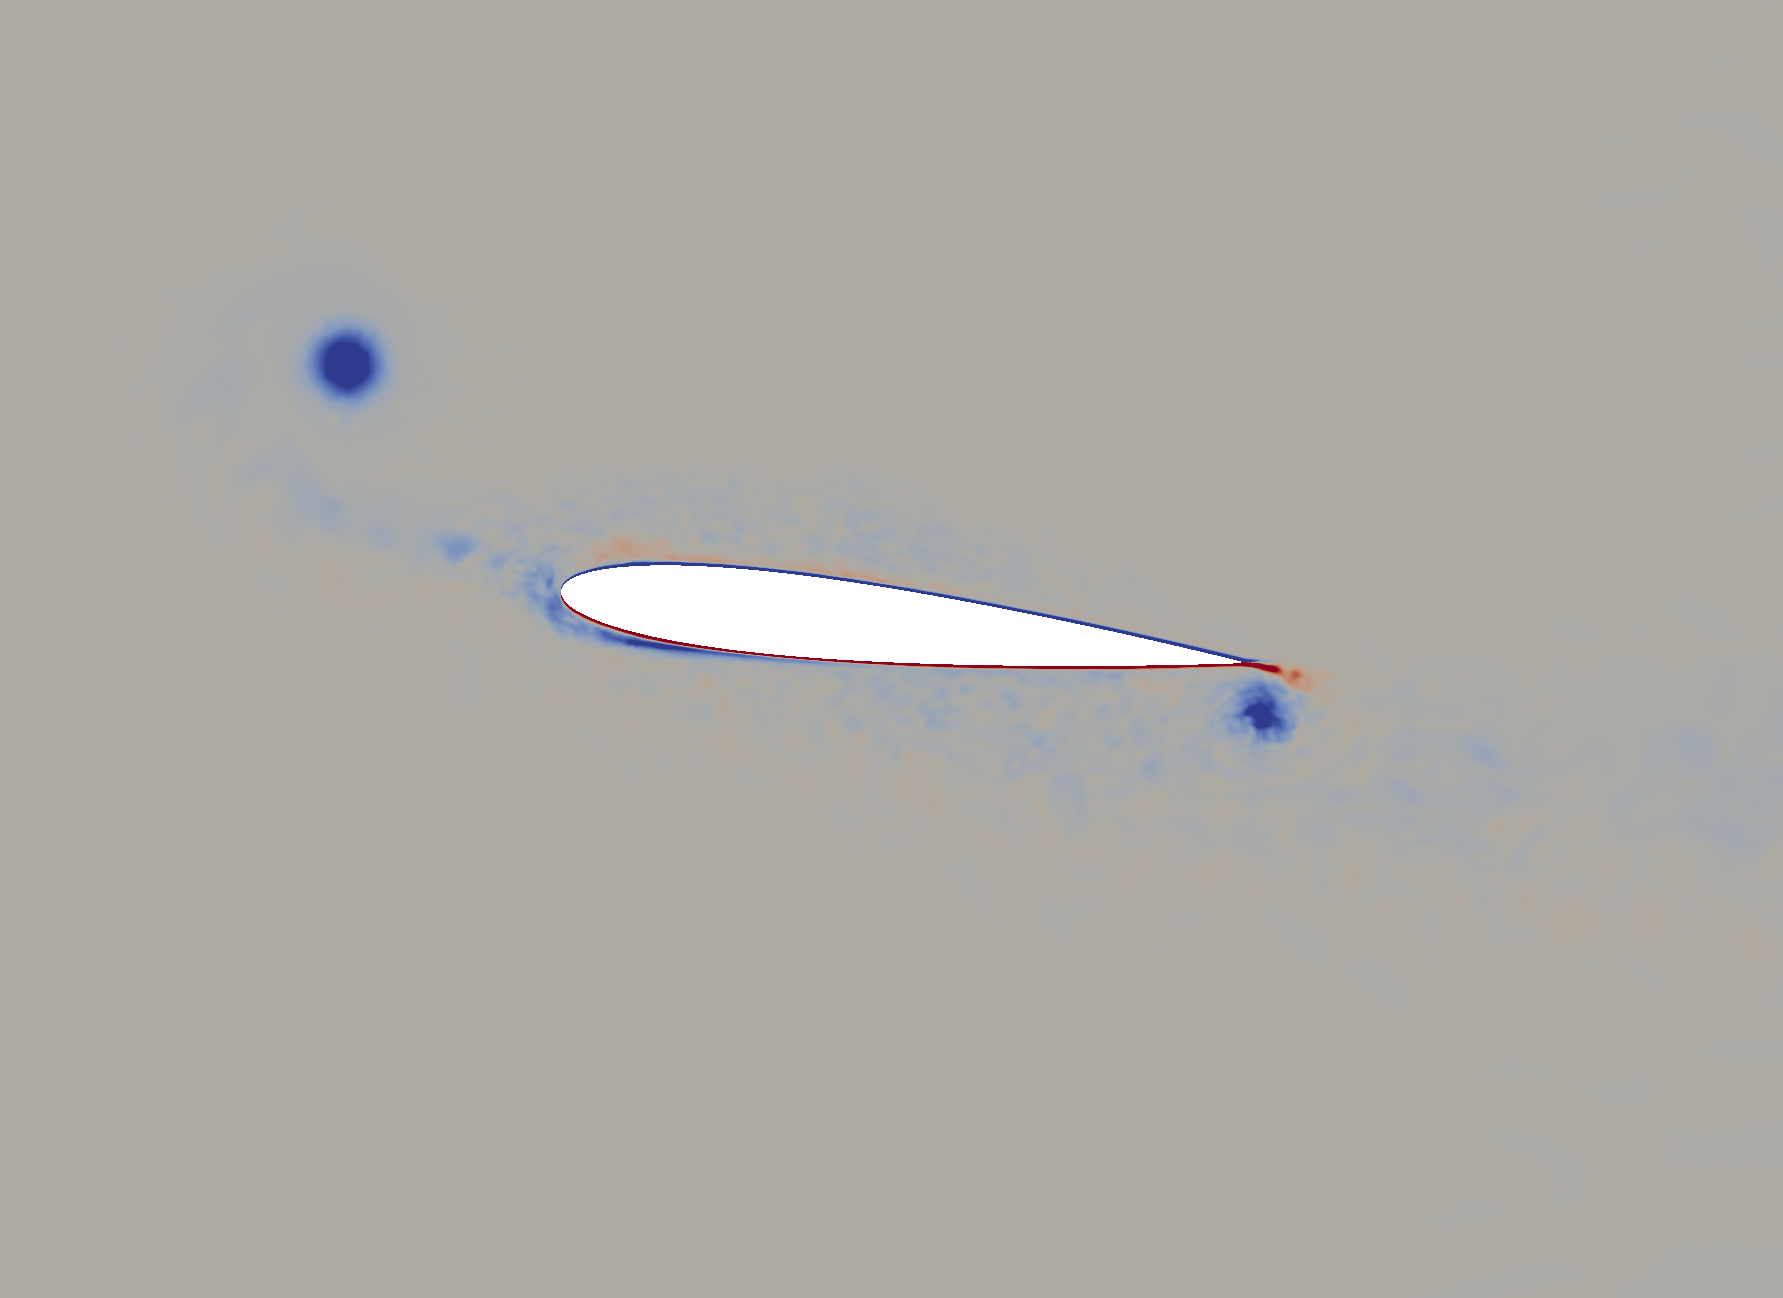
\includegraphics[width=1\textwidth]{figures/Vorticity_plots/Re_200k_1pt2/phase_315.png}
		\caption{$Re=2e5$, $\psi$ = $315^\circ$, $\tilde{t}=0.875$}
		\label{fig:Re_200k_1pt2_phi315}
	\end{subfigure}
	\begin{subfigure}[b]{0.32\textwidth}
		\centering
		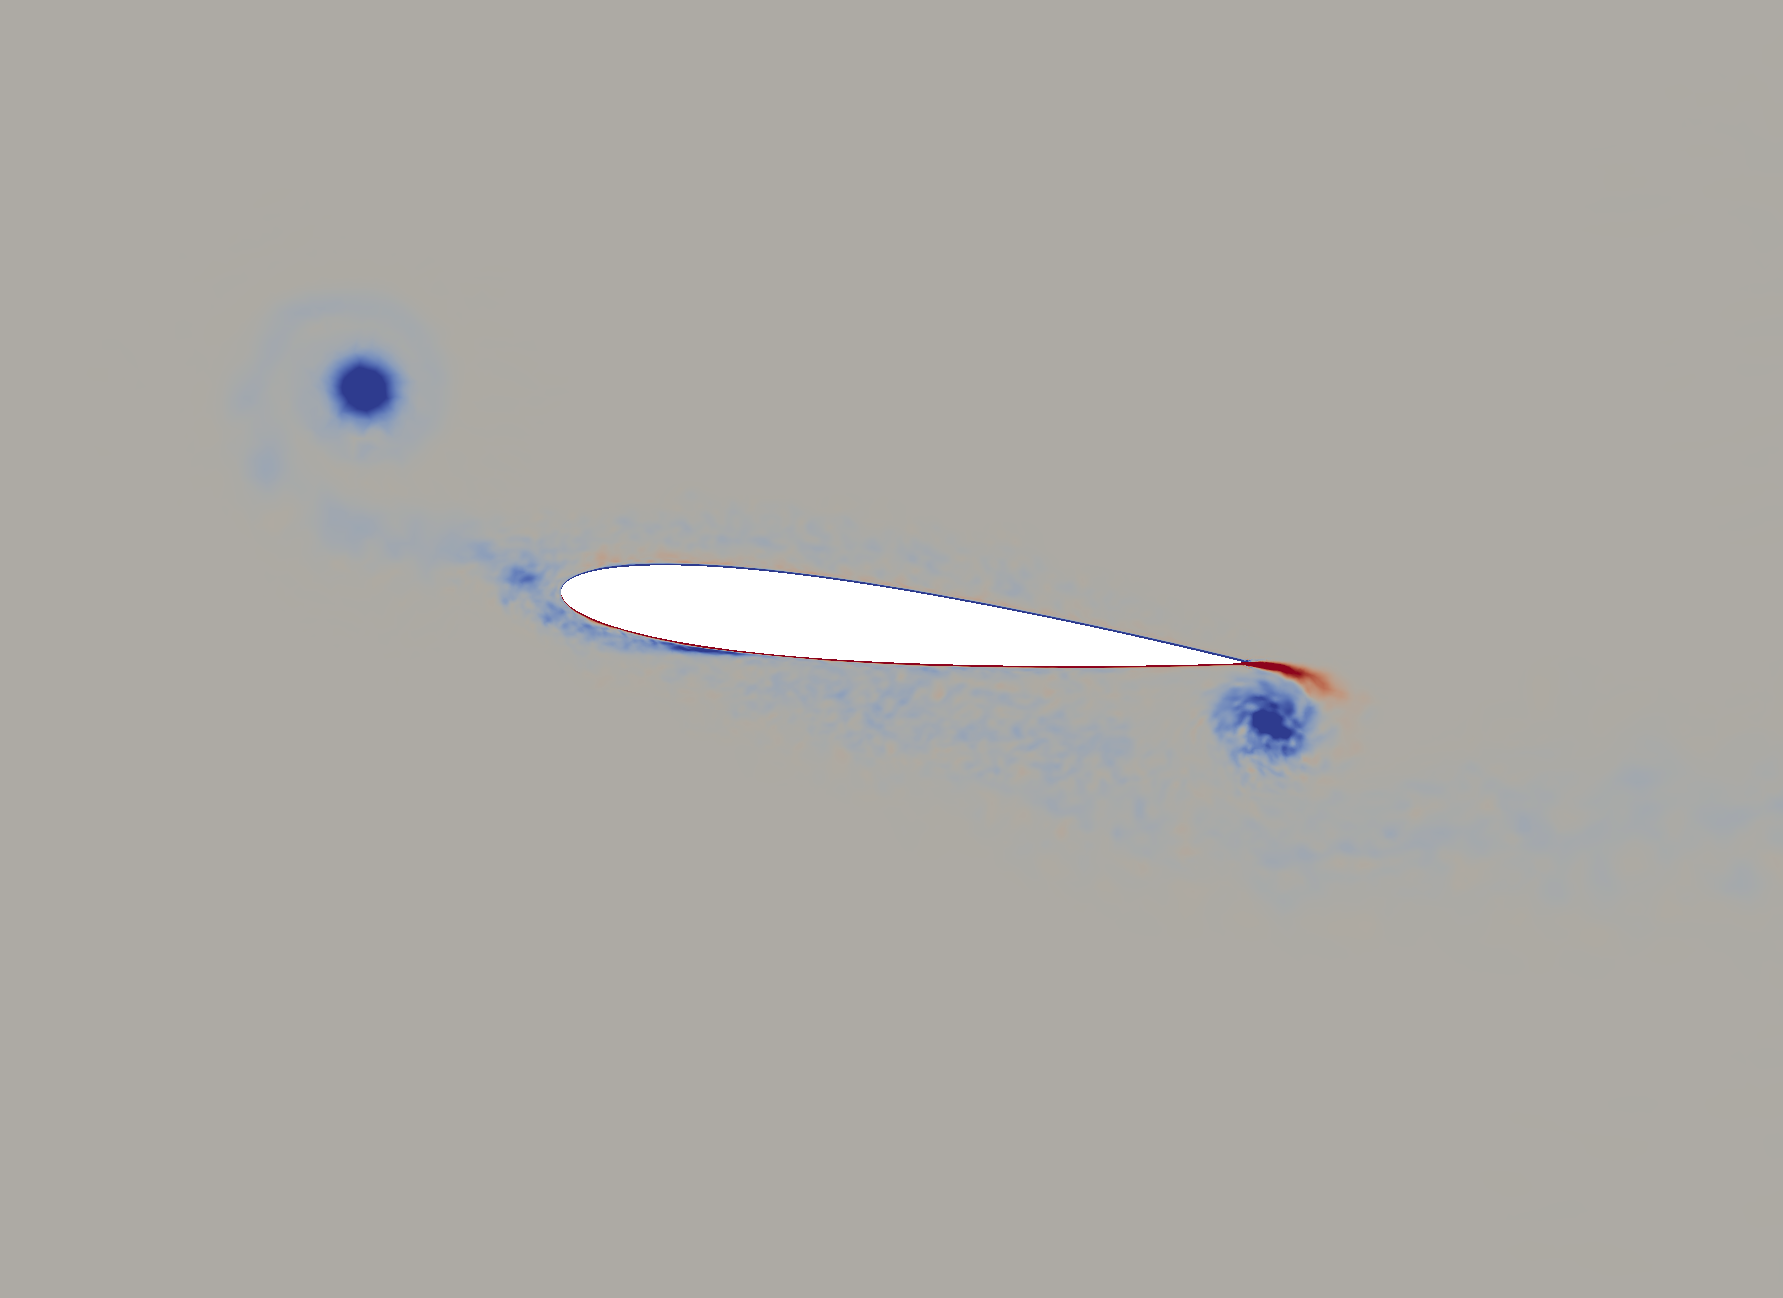
\includegraphics[width=1\textwidth]{figures/Vorticity_plots/Re_1m_1pt2/phase_315.png}
		\caption{$Re=1e6$, $\psi$ = $315^\circ$, $\tilde{t}=0.875$}
		\label{fig:Re_1m_1pt2_phi315}
	\end{subfigure}
	
	\begin{subfigure}[b]{0.32\textwidth}
		\centering
		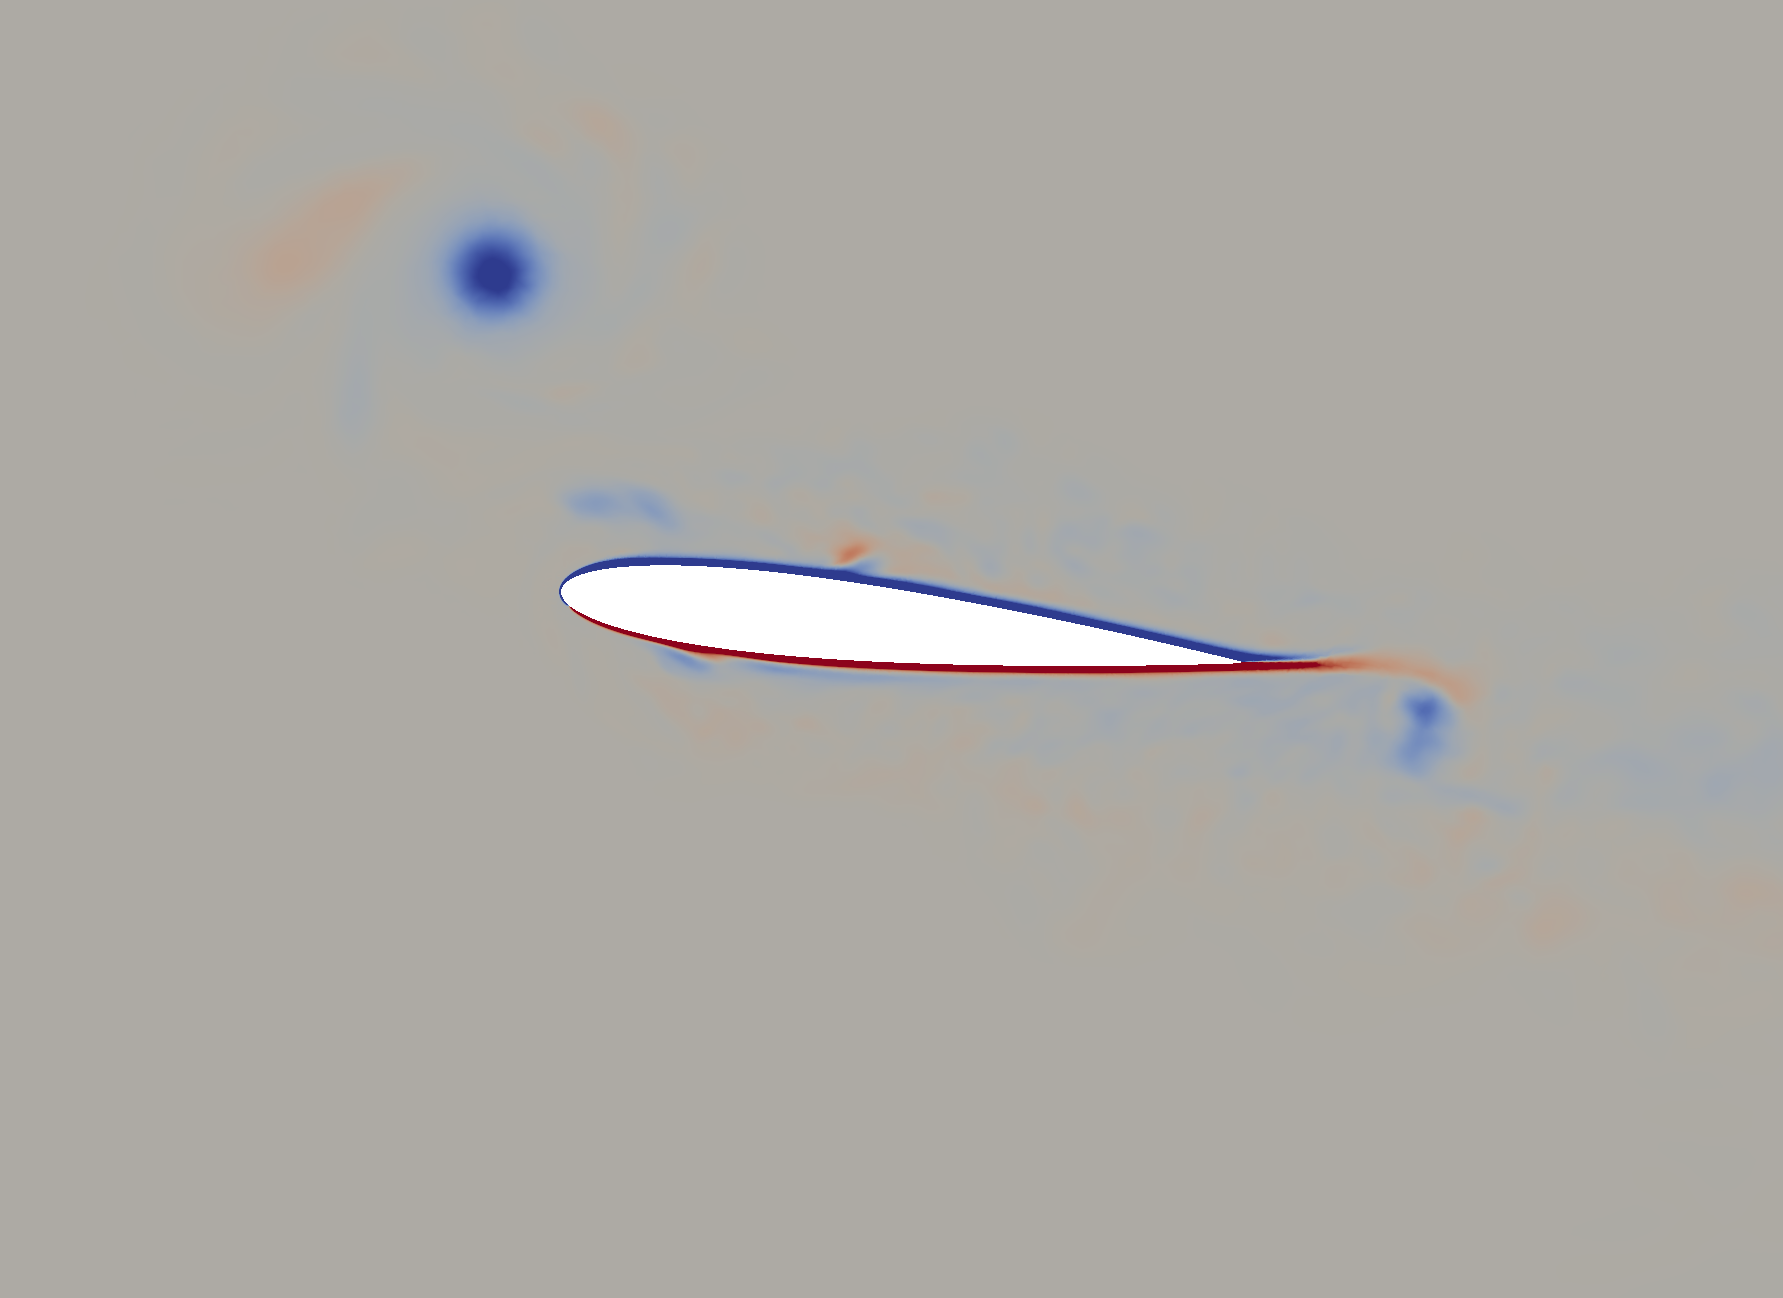
\includegraphics[width=1\textwidth]{figures/Vorticity_plots/Re_40k_1pt2/phase_330.png}
		\caption{$Re=4e4$, $\psi$ = $330^\circ$, $\tilde{t}=0.917$}
		\label{fig:Re_40k_1pt2_phi330}
	\end{subfigure}
	\begin{subfigure}[b]{0.32\textwidth}
		\centering
		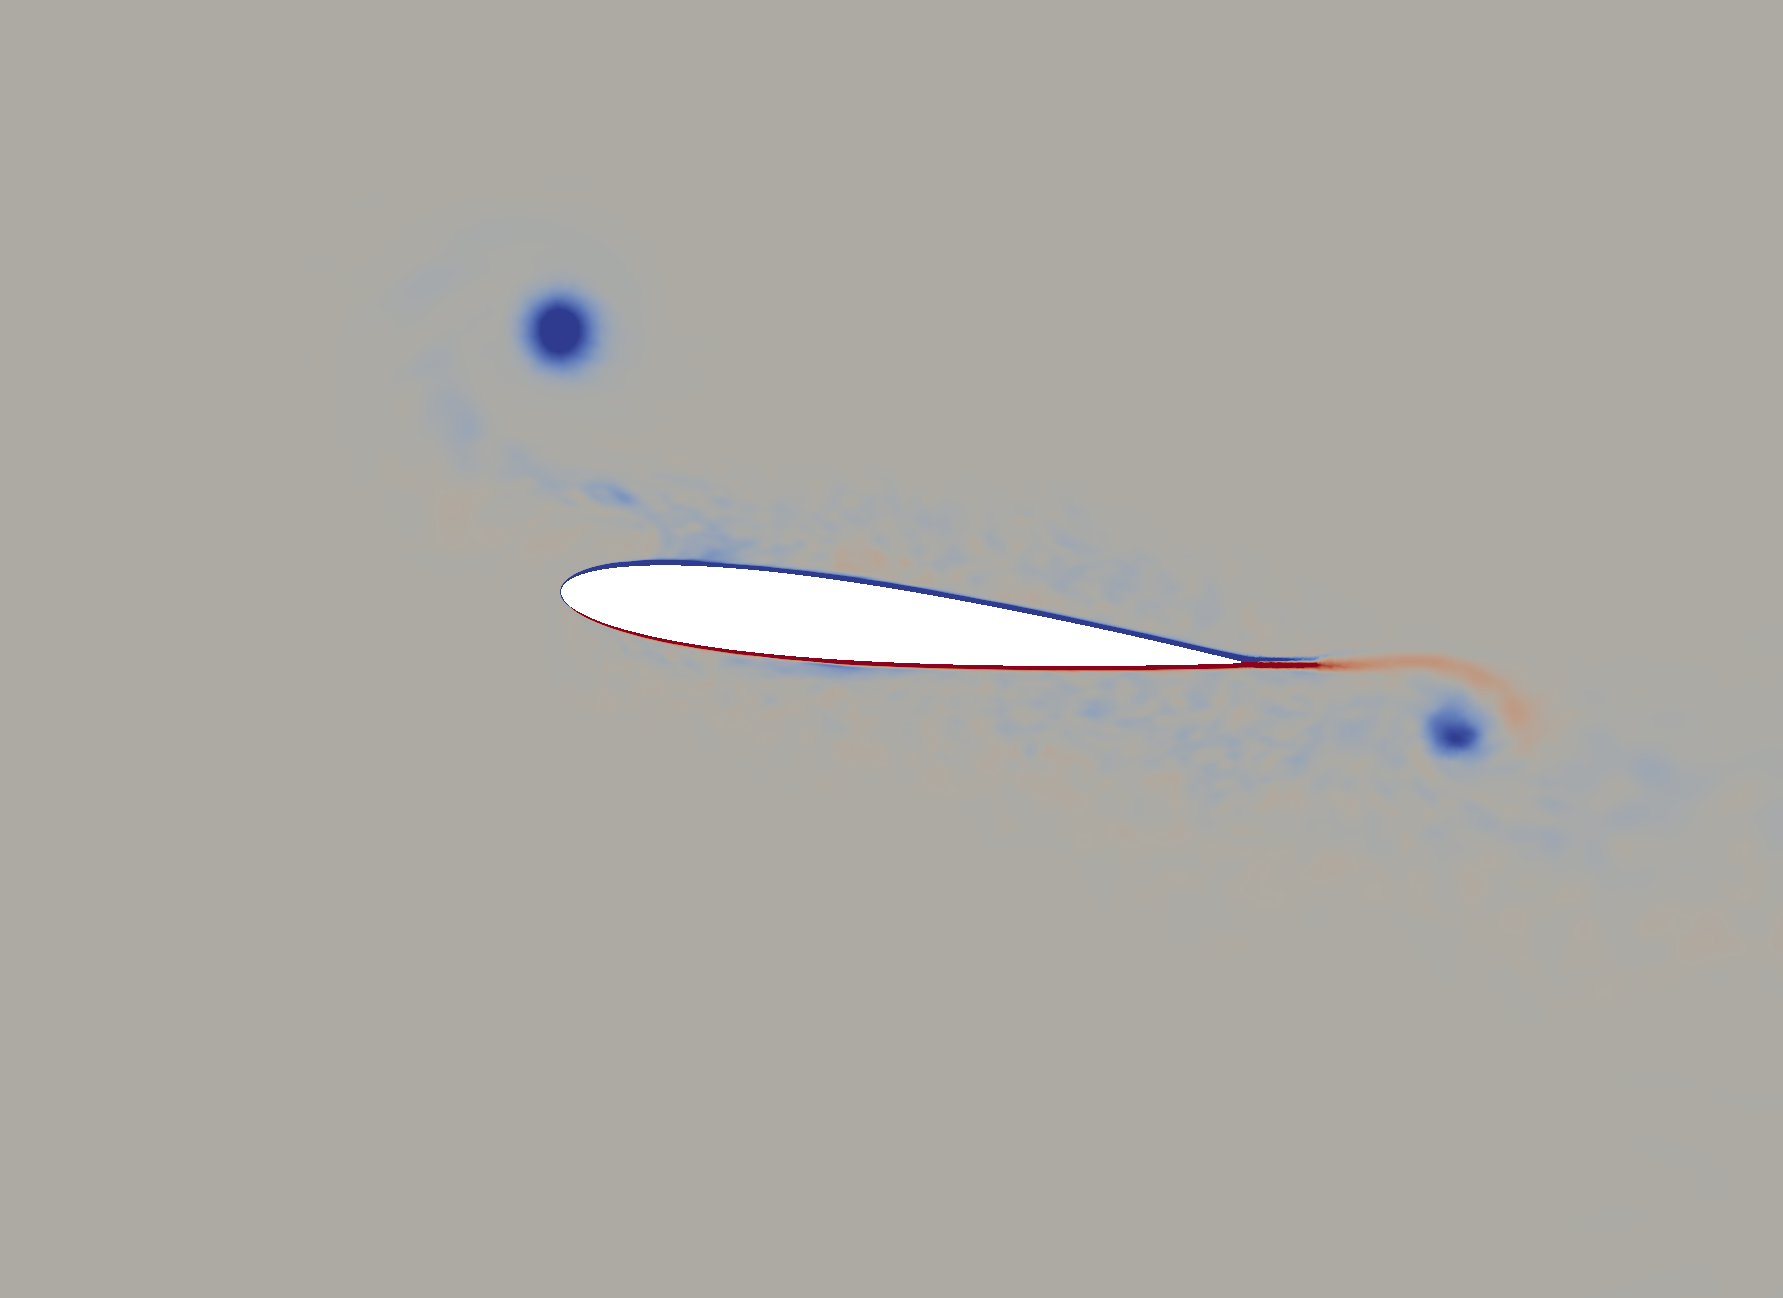
\includegraphics[width=1\textwidth]{figures/Vorticity_plots/Re_200k_1pt2/phase_330.png}
		\caption{$Re=2e5$, $\psi$ = $330^\circ$, $\tilde{t}=0.917$}
		\label{fig:Re_200k_1pt2_phi330}
	\end{subfigure}
	\begin{subfigure}[b]{0.32\textwidth}
		\centering
		\includegraphics[width=1\textwidth]{figures/Vorticity_plots/Re_1m_1pt2/phase_330.png}
		\caption{$Re=1e6$,$\psi$ = $330^\circ$, $\tilde{t}=0.917$}
		\label{fig:Re_1m_1pt2_phi330}
	\end{subfigure}	
	\begin{subfigure}[b]{0.32\textwidth}
		\centering
		\includegraphics[width=1\textwidth]{figures/Vorticity_plots/Re_40k_1pt2/phase_345.png}
		\caption{$Re=4e4$, $\psi$ = $345^\circ$, $\tilde{t}=0.958$}
		\label{fig:Re_40k_1pt2_phi345}
	\end{subfigure}
	\begin{subfigure}[b]{0.32\textwidth}
		\centering
		\includegraphics[width=1\textwidth]{figures/Vorticity_plots/Re_200k_1pt2/phase_345.png}
		\caption{$Re=2e5$, $\psi$ = $345^\circ$, $\tilde{t}=0.958$}
		\label{fig:Re_200k_1pt2_phi345}
	\end{subfigure}
	\begin{subfigure}[b]{0.32\textwidth}
		\centering
		\includegraphics[width=1\textwidth]{figures/Vorticity_plots/Re_1m_1pt2/phase_345.png}
		\caption{$Re=1e6$,$\psi$ = $345^\circ$, $\tilde{t}=0.958$}
		\label{fig:Re_1m_1pt2_phi345}
	\end{subfigure}
	
	\caption{Spanwise vorticity at 8 different phases for $Re$=40,000 (left column), 200,000 (middle column) and 1,000,000 (right column) at $\lambda$ = 1.2}
	\label{fig:vortScreen_1pt2}
\end{figure}

\section{Feature/Vortex Detection and Tracking: LEV}
\label{sec:LEV}

In this section, we quantify the evolution of the LEV based on its size and position.
In order to do so, for each case at first the phase of formation of the LEV is detected and in subsequent phases the LEV is tracked.
Pressure and velocity data is analyzed to automatically detect the formation of the LEV.
In the retreating portion of the cycle, location with minimum pressure is determined starting at $\psi=180^\circ$.
The first phase at which the minimum pressure location is off the airfoil surface (i.e., away from the airfoil and into the flow) is tagged to be a potential phase for LEV formation.
At this potential phase, velocity profile is obtained over multiple lines passing through the minimum pressure location.
These are radial lines that are taken at an equispaced interval along the azimuth in the plane of the airfoil (note that the data is averaged in the spanwise direction).
Along these lines, at first a relative velocity is computed with respect to the velocity at the minimum pressure location.
Subsequently, normal component of the relative velocity is obtained (i.e., normal to each line), which is the azimuthal or tangential component in the polar coordinate system centered around the minimum pressure location.
The azimuthal component (of the relative velocity) is analyzed against the velocity profile of a Lamb-Oseen vortex.
It is noteworthy that the azimuthal component of the relative velocity along several radial lines at multiple phases in the surging cycle were visually analyzed for different cases and found to fit the Lamb-Oseen vortex model fairly well.


LEV position with respect to the leading edge of the airfoil is presented in Figure~\ref{fig:LEV_location_LE_airfoil}.
In the $\mu_{sect}=1.0$ case, the initial position of the LEV (i.e., position at formation) gets closer to the leading edge as the Reynolds number is increased.
Further, LEV remains closest to the airfoil over the cycle for the highest Reynolds number of $Re$=1,000,000 (i.e., note the vertical position of the LEV).
On the other hand, LEV initially moves to the left (towards the geometric leading edge) from its initial position for the lowest Reynolds number of $Re$=40,000.
In the $\mu_{sect}=1.2$ case also, similar trends are observed.
However, at the higher advance ratio the LEV initially moves to the left past the geometric leading edge for each Reynolds number.
This is expected since the relative flow velocity becomes negative (or a reversed flow condition is obtained) at $\mu_{sect}=1.2$.

Figure \ref{fig:LEV_size} presents the size or core radius ($r_c$) of the LEV for all six cases.
We note that in simulations the data was recorded at every $\Delta \psi = 15^\circ$ starting at $\psi$=$15^\circ$.
For each case the LEV is formed at about $\tilde{t}=0.6$ or later.
The LEV size is higher for the lowest Reynolds number of $Re$=40,000 for both advance ratios of $\mu_{sect}$=1.0 and 1.2.
This is expected since the boundary layer is thicker for $Re$=40,000 and the resulting separated shear layer rolls up into a larger LEV.
The LEV size is very similar for the other two higher Reynolds numbers at $\mu_{sect}$=1.0 and 1.2.
In the $\mu_{sect}$=1.0 case, the LEV increases in size till about $\tilde{t}=0.75$ to 0.8 and subsequently seem to plateau or increase in size relatively slowly.
Towards the end of the cycle, the LEV size is about 8\% of the chord for $Re$=40,000 at $\mu_{sect}$=1.0, and about 6\% for $Re$=200,000 and 1,000,000 at $\mu_{sect}$=1.0.
In the $\mu_{sect}$=1.2 case, the LEV increases in size throughout the cycle and towards the end of the cycle reaches about a similar size as the $\mu_{sect}$=1.0 case for each Reynolds number.

\begin{figure}[H]
	\begin{subfigure}{0.5\textwidth}
		\includegraphics[width=1\textwidth]{figures/LEV_size_lambda_1pt0.png}
		\caption{$\mu_{sect} = 1.0$}
		\label{fig:LEV_size_lambda_1p0}
	\end{subfigure}
 	\begin{subfigure}{0.5\textwidth}
	\includegraphics[width=1\textwidth]{figures/LEV_size_lambda_1pt2.png}
	\caption{$\mu_{sect} = 1.2$}
	\label{fig:LEV_size_lambda_1p2}
	\end{subfigure}
 	\caption{LEV size for $Re$=40,000 (green line with open triangles), 200,000 (red line with closed circles) and 1,000,000 (blue line with open circles) at $\mu_{sect}$=1.0 and 1.2}
 	\label{fig:LEV_size}
\end{figure}


This feature/vortex detection and tracking procedure is useful for feature-based adaptivity, which is discussed in Section \ref{sec:feature_based_strat}.

%TODO: indicate we consider Re=40k and 200k for adaptive LES and carefully investigate mesh convergence. this was done for cost savings since LEV exhibits a similar behavior for Re=200k and Re=1m cases.

\begin{figure}[H]
	\begin{subfigure}{0.5\textwidth}
		\includegraphics[width=1\textwidth]{figures/LEV_location_lambda_1pt0}
		\caption{$\mu_{sect} = 1.0$}
		\label{fig:LEV_location_lambda_1p0}
	\end{subfigure}
	\begin{subfigure}{0.5\textwidth}
		\includegraphics[width=1\textwidth]{figures/LEV_location_lambda_1pt2}
		\caption{$\mu_{sect} = 1.2$}
		\label{fig:LEV_location_lambda_1p2}
	\end{subfigure}
 	\caption{LEV position (with respect to the leading edge of the airfoil) for $Re$=40,000 (green line with open triangles), 200,000 (red line with closed circles) and 1,000,000 (blue line with open circles) at $\mu_{sect}$=1.0 and 1.2}
	\label{fig:LEV_location_LE_airfoil}
\end{figure}

\section{Active Reflex Camber}
In this section, we focus only on high Reynolds number flow ($Re=1,000,000$) at higher angle of attack of $\alpha=10^\circ$ and section advance ratios of $\mu_{sect}= 1.5$ and $2.0$. These advance ratios include a significant portion of the retreating phase with negative relative velocity or a reversed flow condition. 
In this reverse flow condition, massive flow separation near the geometric trailing edge is observed, and as a result, a force is experienced by the airfoil along the surging direction. We try to mitigate this by applying active flow control in the form of active reflex camber. 

The case with active reflex camber is referred as the actuated case.
In the actuated case, the (geometric) trailing edge is deflected up by an angle of $\beta_{TE}$=$\alpha$=10$^\circ$, with the hinge point at the 3/4th or 75\% chord location (i.e., close to the trailing edge).
The reflex camber is applied smoothly over a short period of time (both at activation and deactivation).
The full reflex/deflection is achieved just before the reverse flow regime is encountered by the airfoil in the retreating phase, and the airfoil starts to return to its original/undeflected shape once the airfoil is out of the reverse flow.

Figure \ref{fig:U_rel} shows the variation of $\tilde{U}_{rel}$ over the cycle at sectional advance ratio of $\mu_{sect}=1.5$ (blue dashed line) and $2.0$ (green solid line). The region with $\tilde{U}_{rel}<0$ shows the phases when reverse flow is encountered by the airfoil. The open circles on each curve represent the portion of the oscillation cycle when reflex camber is activated for that particular sectional advance ratio.


\begin{figure}[H]
	\begin{center}
\texttt{}		\includegraphics[width=4in]{figures/U_rel_vs_t_tilde_without_lines.png}
		\caption{Variation of $\tilde{U}_{rel}$ at $\mu_{sect}=1.5$ (green solid line) and $2.0$ (blue dashed line), open circles on each curve represent the portion of the oscillation cycle when reflex camber is activated}
		% with $\tilde{t}$ for $\lambda = 1.5$; shaded region where actuated camber is employed; red vertical lines showing instances where data is captured}
		\label{fig:U_rel}
	\end{center}
\end{figure}



Table~\ref{table:summary_cases_AC} provides a summary of the current cases. $\beta_{TE}=0$ refers to the non-actuated case while $\beta_{TE}=\alpha$ is the actuated case.

\begin{table}[H]
	\centering
	\caption{Summary of cases}
	\label{table:summary_cases_AC}
	\begin{tabular}{|l|c|c|c|c|c|}
		\hline
		Airfoil   & $\alpha$ & $k$ & $\mu_{sect}$ & $Re$ (mean) & $\beta_{TE}$\\
		\hline
		\hline
		NACA 0012 & 10$^\circ$ & $0.133$ & \{1.5, 2.0\} & 1,000,000 & \{0,$\alpha$\} \\
		\hline
		
	\end{tabular}
	
\end{table}

The computational domain and boundary conditions for this case are similar to the one mentioned in Section \ref{sec:baseline_cases}.
Also, as noted earlier, an ALE description is used to account for the motion and deformation of the airfoil.
Mesh deformation is currently prescribed based on the motion and deformation of the airfoil.
The deformed mesh due to active reflex camber is shown in Figure \ref{fig:mesh3}.

The computational domain and boundary conditions for this case are similar to the one mentioned in Section \ref{sec:baseline_cases}.
Also, as noted earlier, an ALE description is used to account for the motion and deformation of the airfoil.
Mesh deformation is currently prescribed based on the motion and deformation of the airfoil.
The deformed mesh due to active reflex camber is shown in Figure \ref{fig:mesh3}.


\begin{figure}[H]
	\centering
	\begin{subfigure}[b]{0.4\textwidth}
		\centering
		\includegraphics[width=1\textwidth]{figures/Setup/mesh}
		\caption{non-actuated case}
		\label{fig:mesh_non-actuated}
	\end{subfigure}
%	\begin{subfigure}[b]{0.4\textwidth}
%		\centering
%		\includegraphics[width=1\textwidth]{figures/Setup/mesh_AC}
%		\caption{actuated case (with reflex camber)}
%		\label{fig:mesh_actuated}
%	\end{subfigure}
	\caption{Mesh around the airfoil for the non-actuated and actuated cases during the reverse flow region}
	\label{fig:mesh3}
\end{figure}


Figure \ref{fig:vortScreen_mu1pt5} shows the instantaneous spanwise vorticity for the sectional advance ratio of $\mu_{sect}$=1.5.
8 different phases over the retreating phase of the oscillation cycle are shown. The vorticity range is selected to be [-30,30]$ U_{sect}/C$. For this sectional advance ratio, the airfoil enters the reverse flow region around $\psi=222^\circ$ and exits the reverse flow region at about $\psi$=$318^\circ$. In the actuated case, reflex camber is activated at $\psi$=$215^\circ$, and smoothly reaches the full deflection at $\psi$=$220^\circ$. After the airfoil exits the reverse flow, the reflexed airfoil starts returning to its undeflected position at $\psi$=$320^\circ$, and smoothly reaches its original shape at $\psi$=$325^\circ$.


At $\psi$=$195^\circ$, the flow over the airfoil is very similar between the baseline and actuated cases.
At $\psi$=$225^\circ$ for the actuated case, reflex camber is fully activated as seen in Figure \ref{fig:mu_1pt5_AC_psi225}. As the trailing edge is deflected upwards, a small vortex is formed just below it. Also, a roll up of the boundary layer is observed near the geometric leading edge for both baseline and actuated cases, and the formation of the leading edge vortex (LEV) begins. A more detailed analysis of the LEV at different Reynolds numbers and advance ratios was reported in \ref{sec:baseline_results}.

At $\psi$=$240^\circ$, flow separation forms near the bottom of the trailing edge of the airfoil for both baseline and actuated cases.
In the subsequent phases of the baseline case, the extent of this separated region increases along the airfoil and in the transverse direction, i.e., the separation bubble grows, till up to $\psi$=$285^\circ$. 
On the contrary, the extent of the separated region remains relatively small in the actuated case. For example, see Figures \ref{fig:mu_1pt5_baseline_psi285} and \ref{fig:mu_1pt5_AC_psi285}.
Moreover, in the actuated case the size of the separated region remains fairly constant between phases $\psi$=$255^\circ$ and $285^\circ$, see Figures \ref{fig:mu_1pt5_AC_psi255}, \ref{fig:mu_1pt5_AC_psi270} and \ref{fig:mu_1pt5_AC_psi285}.
Overall a significant reduction is observed in the size/extent as well as unsteadiness of the separation bubble near the trailing edge during the reverse flow region due to active reflex camber.
The implications of this trailing-edge separated region on the drag force is discussed in Section \ref{sec:drag_profile}

After $\psi$=$285^\circ$, the trailing-edge flow separation begins to wash away from the airfoil for both baseline and actuated cases.
For the actuated case at $\psi$=$330^\circ$, the reflexed trailing edge is at its undeflected position.
As the trailing edge is deflected down to its original position, this results in the formation of another small vortex as seen in Figure \ref{fig:mu_1pt5_AC_psi330}, similar to when the trailing edge is deflected up (e.g., at $\psi$=$225^\circ$ in Figure \ref{fig:mu_1pt5_AC_psi225}).

\begin{figure}[H]
	\centering
	
	\begin{subfigure}[b]{0.4\textwidth}
		\centering
		\includegraphics[width=1\textwidth]{figures/mu_1pt5/vorticity/baseline/phase_195.png}
		\caption{ $\psi$ = $195^\circ$, $\tilde{t}=0.542$}
		\label{fig:mu_1pt5_baseline_psi195}
	\end{subfigure}
	\begin{subfigure}[b]{0.4\textwidth}
		\centering
		\includegraphics[width=1\textwidth]{figures/mu_1pt5/vorticity/AC/phase_195.png}
		\caption{ $\psi$ = $195^\circ$, $\tilde{t}=0.542$}
		\label{fig:mu_1pt5_AC_psi195}
	\end{subfigure}
	
	%\begin{subfigure}[b]{0.4\textwidth}
	%	\centering
	%	\includegraphics[width=1\textwidth]{figures/mu_1pt5/vorticity/baseline/phase_210.png}
	%	\caption{ $\psi$ = $210^\circ$, $\tilde{t}=0.583$}
	%	\label{fig:mu_1pt5_baseline_psi210}
	%\end{subfigure}
	%\begin{subfigure}[b]{0.4\textwidth}
	%	\centering
	%	\includegraphics[width=1\textwidth]{figures/mu_1pt5/vorticity/AC/phase_210.png}
	%	\caption{ $\psi$ = $210^\circ$, $\tilde{t}=0.583$}
	%	\label{fig:mu_1pt5_AC_psi210}
	%\end{subfigure}
	
	\begin{subfigure}[b]{0.4\textwidth}
		\centering
		\includegraphics[width=1\textwidth]{figures/mu_1pt5/vorticity/baseline/phase_225.png}
		\caption{ $\psi$ = $225^\circ$, $\tilde{t}=0.625$}
		\label{fig:mu_1pt5_baseline_psi225}
	\end{subfigure}
	\begin{subfigure}[b]{0.4\textwidth}
		\centering
		\includegraphics[width=1\textwidth]{figures/mu_1pt5/vorticity/AC/phase_225.png}
		\caption{ $\psi$ = $225^\circ$,  $\tilde{t}=0.625$}
		\label{fig:mu_1pt5_AC_psi225}
	\end{subfigure}
	
	
	\begin{subfigure}[b]{0.4\textwidth}
		\centering
		\includegraphics[width=1\textwidth]{figures/mu_1pt5/vorticity/baseline/phase_240.png}
		\caption{ $\psi$ = $240^\circ$, $\tilde{t}=0.667$}
		\label{fig:mu_1pt5_baseline_psi240}
	\end{subfigure}
	\begin{subfigure}[b]{0.4\textwidth}
		\centering
		\includegraphics[width=1\textwidth]{figures/mu_1pt5/vorticity/AC/phase_240.png}
		\caption{ $\psi$ = $240^\circ$, $\tilde{t}=0.667$}
		\label{fig:mu_1pt5_AC_psi240}
	\end{subfigure}
	
	\begin{subfigure}[b]{0.4\textwidth}
		\centering
		\includegraphics[width=1\textwidth]{figures/mu_1pt5/vorticity/baseline/phase_255.png}
		\caption{ $\psi$ = $255^\circ$, $\tilde{t}=0.708$}
		\label{fig:mu_1pt5_baseline_psi255}
	\end{subfigure}
	\begin{subfigure}[b]{0.4\textwidth}
		\centering
		\includegraphics[width=1\textwidth]{figures/mu_1pt5/vorticity/AC/phase_255.png}
		\caption{ $\psi$ = $255^\circ$, $\tilde{t}=0.708$}
		\label{fig:mu_1pt5_AC_psi255}
	\end{subfigure}
	
	
	\caption{Instantaneous spanwise vorticity at 8 different phases for the baseline (left column) and actuated (right column) cases at $\mu_{sect}$ = 1.5}
	%\label{fig:vortScreen_mu1pt5}
\end{figure}

\begin{figure}[H]\ContinuedFloat
	\centering
	
	\begin{subfigure}[b]{0.4\textwidth}
		\centering
		\includegraphics[width=1\textwidth]{figures/mu_1pt5/vorticity/baseline/phase_270.png}
		\caption{ $\psi$ = $270^\circ$, $\tilde{t}=0.75$}
		\label{fig:mu_1pt5_baseline_psi270}
	\end{subfigure}
	\begin{subfigure}[b]{0.4\textwidth}
		\centering
		\includegraphics[width=1\textwidth]{figures/mu_1pt5/vorticity/AC/phase_270.png}
		\caption{ $\psi$ = $270^\circ$, $\tilde{t}=0.75$}
		\label{fig:mu_1pt5_AC_psi270}
	\end{subfigure}
	
	\begin{subfigure}[b]{0.4\textwidth}
		\centering
		\includegraphics[width=1\textwidth]{figures/mu_1pt5/vorticity/baseline/phase_285.png}
		\caption{ $\psi$ = $285^\circ$, $\tilde{t}=0.792$}
		\label{fig:mu_1pt5_baseline_psi285}
	\end{subfigure}
	\begin{subfigure}[b]{0.4\textwidth}
		\centering
		\includegraphics[width=1\textwidth]{figures/mu_1pt5/vorticity/AC/phase_285.png}
		\caption{ $\psi$ = $285^\circ$,  $\tilde{t}=0.792$}
		\label{fig:mu_1pt5_AC_psi285}
	\end{subfigure}
	
	
	%\begin{subfigure}[b]{0.4\textwidth}
	%	\centering
	%	\includegraphics[width=1\textwidth]{figures/mu_1pt5/vorticity/baseline/phase_300.png}
	%	\caption{ $\psi$ = $300^\circ$, $\tilde{t}=0.833$}
	%	\label{fig:mu_1pt5_baseline_psi300}
	%\end{subfigure}
	%\begin{subfigure}[b]{0.4\textwidth}
	%	\centering
	%	\includegraphics[width=1\textwidth]{figures/mu_1pt5/vorticity/AC/phase_300.png}
	%	\caption{ $\psi$ = $300^\circ$, $\tilde{t}=0.833$}
	%	\label{fig:mu_1pt5_AC_psi300}
	%\end{subfigure}
	
	\begin{subfigure}[b]{0.4\textwidth}
		\centering
		\includegraphics[width=1\textwidth]{figures/mu_1pt5/vorticity/baseline/phase_315.png}
		\caption{ $\psi$ = $315^\circ$, $\tilde{t}=0.875$}
		\label{fig:mu_1pt5_baseline_psi315}
	\end{subfigure}
	\begin{subfigure}[b]{0.4\textwidth}
		\centering
		\includegraphics[width=1\textwidth]{figures/mu_1pt5/vorticity/AC/phase_315.png}
		\caption{ $\psi$ = $315^\circ$, $\tilde{t}=0.875$}
		\label{fig:mu_1pt5_AC_psi315}
	\end{subfigure}
	
	\begin{subfigure}[b]{0.4\textwidth}
		\centering
		\includegraphics[width=1\textwidth]{figures/mu_1pt5/vorticity/baseline/phase_330.png}
		\caption{ $\psi$ = $330^\circ$, $\tilde{t}=0.917$}
		\label{fig:mu_1pt5_baseline_psi330}
	\end{subfigure}
	\begin{subfigure}[b]{0.4\textwidth}
		\centering
		\includegraphics[width=1\textwidth]{figures/mu_1pt5/vorticity/AC/phase_330.png}
		\caption{ $\psi$ = $330^\circ$, $\tilde{t}=0.917$}
		\label{fig:mu_1pt5_AC_psi330}
	\end{subfigure}
	
	%\begin{subfigure}[b]{0.4\textwidth}
	%	\centering
	%	\includegraphics[width=1\textwidth]{figures/mu_1pt5/vorticity/baseline/phase_345.png}
	%	\caption{ $\psi$ = $345^\circ$, $\tilde{t}=0.958$}
	%	\label{fig:mu_1pt5_baseline_psi345}
	%\end{subfigure}
	%\begin{subfigure}[b]{0.4\textwidth}
	%	\centering
	%	\includegraphics[width=1\textwidth]{figures/mu_1pt5/vorticity/AC/phase_345.png}
	%	\caption{ $\psi$ = $345^\circ$, $\tilde{t}=0.958$}
	%	\label{fig:mu_1pt5_AC_psi345}
	%\end{subfigure}
	
	
	
	\caption{Instantaneous spanwise vorticity at 8 different phases for the baseline (left column) and actuated (right column) cases at $\mu_{sect}$ = 1.5}
	\label{fig:vortScreen_mu1pt5}
\end{figure}



Figure \ref{fig:vortScreen_mu2pt0} shows the instantaneous spanwise vorticity for the sectional advance ratio of $\mu_{sect}=2.0$.
As before, 8 different phases over the retreating phase of the cycle are shown and the vorticity range is selected to be [-30,30]$ U_{sect} /C$. Note that the set of phases shown is different between $\mu_{sect}=1.5$ and $2.0$. For this advance ratio, the airfoil enters the reverse flow region at $\psi=210^\circ$, and exits the reverse flow at $\psi=330^\circ$.
Reflex camber is activated at the phase of $\psi$=$200^\circ$ and reaches the full deflection at $\psi$=$205^\circ$.
After the airfoil exits the reverse flow, the reflexed airfoil starts returning to its undeflected position at $\psi$=$335^\circ$, and smoothly reaches its original shape at $\psi$=$340^\circ$.

As the airfoil trailing edge is deflected upwards for this actuated case with $\mu_{sect}=2.0$, a small vortex is formed near it, see Figure \ref{fig:mu_2pt0_AC_psi210}, which is similar to the actuated case with $\mu_{sect}=1.5$. Roll up of the boundary layer and LEV formation is seen for both baseline and actuated cases at $\psi$=$210^\circ$.
The flow separation near the trailing edge starts to form at an earlier phase of $\psi$=$225^\circ$, as compared to $\psi$=$240^\circ$ for the lower sectional advance ratio of $\mu_{sect}=1.5$.

In the subsequent phases after $\psi$=$225^\circ$ the size of the separated region increases for the baseline case till up to $\psi$=$285^\circ$. However, the separation bubble is larger in the baseline case with $\mu_{sect}=2.0$ as compared to that with $\mu_{sect}=1.5$.
For the actuated case, the separated region is relatively small (see Figures \ref{fig:mu_2pt0_baseline_psi270} and \ref{fig:mu_2pt0_AC_psi270}) and its size remains fairly constant between phases $\psi$=$255^\circ$ and $285^\circ$ (see Figures \ref{fig:mu_2pt0_AC_psi255}, \ref{fig:mu_2pt0_AC_psi270} and \ref{fig:mu_2pt0_AC_psi285}).
As before, overall a significant reduction is observed in the size/extent as well as unsteadiness of the separation bubble near the trailing edge during the reverse flow region due to active reflex camber.
The implications of this trailing-edge separated region on the drag force is discussed in Section \ref{sec:drag_profile}.

After $\psi$=$285^\circ$, the trailing-edge flow separation begins to wash away from the airfoil for both baseline and actuated cases, see Figures \ref{fig:mu_2pt0_baseline_psi315} and \ref{fig:mu_2pt0_AC_psi315}. 
For the actuated case at $\psi$=$345^\circ$, the reflexed trailing edge is at its undeflected position.
As the trailing edge is deflected down to its original position, this results in the formation of a small vortex as seen in Figure \ref{fig:mu_2pt0_AC_psi345}.

\begin{figure}[H]
	\centering
	
	\begin{subfigure}[b]{0.4\textwidth}
		\centering
		\includegraphics[width=1\textwidth]{figures/mu_2pt0/vorticity/baseline/phase_195.png}
		\caption{ $\psi$ = $195^\circ$, $\tilde{t}=0.542$}
		\label{fig:mu_2pt0_baseline_psi195}
	\end{subfigure}
	\begin{subfigure}[b]{0.4\textwidth}
		\centering
		\includegraphics[width=1\textwidth]{figures/mu_2pt0/vorticity/AC/phase_195.png}
		\caption{ $\psi$ = $195^\circ$, $\tilde{t}=0.542$}
		\label{fig:mu_2pt0_AC_psi195}
	\end{subfigure}
	
	\begin{subfigure}[b]{0.4\textwidth}
		\centering
		\includegraphics[width=1\textwidth]{figures/mu_2pt0/vorticity/baseline/phase_210.png}
		\caption{ $\psi$ = $210^\circ$, $\tilde{t}=0.542$}
		\label{fig:mu_2pt0_baseline_psi210}
	\end{subfigure}
	\begin{subfigure}[b]{0.4\textwidth}
		\centering
		\includegraphics[width=1\textwidth]{figures/mu_2pt0/vorticity/AC/phase_210.png}
		\caption{ $\psi$ = $210^\circ$, $\tilde{t}=0.542$}
		\label{fig:mu_2pt0_AC_psi210}
	\end{subfigure}
	
	\begin{subfigure}[b]{0.4\textwidth}
		\centering
		\includegraphics[width=1\textwidth]{figures/mu_2pt0/vorticity/baseline/phase_225.png}
		\caption{ $\psi$ = $225^\circ$, $\tilde{t}=0.625$}
		\label{fig:mu_2pt0_baseline_psi225}
	\end{subfigure}
	\begin{subfigure}[b]{0.4\textwidth}
		\centering
		\includegraphics[width=1\textwidth]{figures/mu_2pt0/vorticity/AC/phase_225.png}
		\caption{ $\psi$ = $225^\circ$,  $\tilde{t}=0.625$}
		\label{fig:mu_2pt0_AC_psi225}
	\end{subfigure}
	
	
	%\begin{subfigure}[b]{0.4\textwidth}
	%	\centering
	%	 \includegraphics[width=1\textwidth]{figures/mu_2pt0/vorticity/baseline/phase_240.png}
	%	\caption{ $\psi$ = $240^\circ$, $\tilde{t}=0.667$}
	%	\label{fig:mu_2pt0_baseline_psi240}
	%\end{subfigure}
	%\begin{subfigure}[b]{0.4\textwidth}
	%	\centering
	%	 \includegraphics[width=1\textwidth]{figures/mu_2pt0/vorticity/AC/phase_240.png}
	%	\caption{ $\psi$ = $240^\circ$, $\tilde{t}=0.667$}
	%	\label{fig:mu_2pt0_AC_psi240}
	%\end{subfigure}
	
	\begin{subfigure}[b]{0.4\textwidth}
		\centering
		\includegraphics[width=1\textwidth]{figures/mu_2pt0/vorticity/baseline/phase_255.png}
		\caption{ $\psi$ = $255^\circ$, $\tilde{t}=0.708$}
		\label{fig:mu_2pt0_baseline_psi255}
	\end{subfigure}
	\begin{subfigure}[b]{0.4\textwidth}
		\centering
		\includegraphics[width=1\textwidth]{figures/mu_2pt0/vorticity/AC/phase_255.png}
		\caption{ $\psi$ = $255^\circ$, $\tilde{t}=0.708$}
		\label{fig:mu_2pt0_AC_psi255}
	\end{subfigure}
	
	
	\caption{Instantaneous spanwise vorticity at 8 different phases for the baseline (left column) and actuated (right column) cases at $\mu_{sect}$ = 2.0}
	%\label{fig:vortScreen_mu2pt0}
\end{figure}

\begin{figure}[H]\ContinuedFloat
	\centering
	
	\begin{subfigure}[b]{0.4\textwidth}
		\centering
		\includegraphics[width=1\textwidth]{figures/mu_2pt0/vorticity/baseline/phase_270.png}
		\caption{ $\psi$ = $270^\circ$, $\tilde{t}=0.75$}
		\label{fig:mu_2pt0_baseline_psi270}
	\end{subfigure}
	\begin{subfigure}[b]{0.4\textwidth}
		\centering
		\includegraphics[width=1\textwidth]{figures/mu_2pt0/vorticity/AC/phase_270.png}
		\caption{ $\psi$ = $270^\circ$, $\tilde{t}=0.75$}
		\label{fig:mu_2pt0_AC_psi270}
	\end{subfigure}
	
	\begin{subfigure}[b]{0.4\textwidth}
		\centering
		\includegraphics[width=1\textwidth]{figures/mu_2pt0/vorticity/baseline/phase_285.png}
		\caption{ $\psi$ = $285^\circ$, $\tilde{t}=0.792$}
		\label{fig:mu_2pt0_baseline_psi285}
	\end{subfigure}
	\begin{subfigure}[b]{0.4\textwidth}
		\centering
		\includegraphics[width=1\textwidth]{figures/mu_2pt0/vorticity/AC/phase_285.png}
		\caption{ $\psi$ = $285^\circ$,  $\tilde{t}=0.792$}
		\label{fig:mu_2pt0_AC_psi285}
	\end{subfigure}
	
	
	%\begin{subfigure}[b]{0.4\textwidth}
	%	\centering
	%	\includegraphics[width=1\textwidth]{figures/mu_2pt0/vorticity/baseline/phase_300.png}
	%	\caption{ $\psi$ = $300^\circ$, $\tilde{t}=0.833$}
	%	\label{fig:mu_2pt0_baseline_psi300}
	%\end{subfigure}
	%\begin{subfigure}[b]{0.4\textwidth}
	%	\centering
	%	\includegraphics[width=1\textwidth]{figures/mu_2pt0/vorticity/AC/phase_300.png}
	%	\caption{ $\psi$ = $300^\circ$, $\tilde{t}=0.833$}
	%	\label{fig:mu_2pt0_AC_psi300}
	%\end{subfigure}
	
	\begin{subfigure}[b]{0.4\textwidth}
		\centering
		\includegraphics[width=1\textwidth]{figures/mu_2pt0/vorticity/baseline/phase_315.png}
		\caption{ $\psi$ = $315^\circ$, $\tilde{t}=0.875$}
		\label{fig:mu_2pt0_baseline_psi315}
	\end{subfigure}
	\begin{subfigure}[b]{0.4\textwidth}
		\centering
		\includegraphics[width=1\textwidth]{figures/mu_2pt0/vorticity/AC/phase_315.png}
		\caption{ $\psi$ = $315^\circ$, $\tilde{t}=0.875$}
		\label{fig:mu_2pt0_AC_psi315}
	\end{subfigure}
	
	%\begin{subfigure}[b]{0.4\textwidth}
	%	\centering
	%	\includegraphics[width=1\textwidth]{figures/mu_2pt0/vorticity/baseline/phase_330.png}
	%	\caption{ $\psi$ = $330^\circ$, $\tilde{t}=0.917$}
	%	\label{fig:mu_2pt0_baseline_psi330}
	%\end{subfigure}
	%\begin{subfigure}[b]{0.4\textwidth}
	%	\centering
	%	\includegraphics[width=1\textwidth]{figures/mu_2pt0/vorticity/AC/phase_330.png}
	%	\caption{ $\psi$ = $330^\circ$, $\tilde{t}=0.917$}
	%	\label{fig:mu_2pt0_AC_psi330}
	%\end{subfigure}
	
	\begin{subfigure}[b]{0.4\textwidth}
		\centering
		\includegraphics[width=1\textwidth]{figures/mu_2pt0/vorticity/baseline/phase_345.png}
		\caption{ $\psi$ = $345^\circ$, $\tilde{t}=0.958$}
		\label{fig:mu_2pt0_baseline_psi345}
	\end{subfigure}
	\begin{subfigure}[b]{0.4\textwidth}
		\centering
		\includegraphics[width=1\textwidth]{figures/mu_2pt0/vorticity/AC/phase_345.png}
		\caption{ $\psi$ = $345^\circ$, $\tilde{t}=0.958$}
		\label{fig:mu_2pt0_AC_psi345}
	\end{subfigure}
	
	
	
	\caption{Instantaneous spanwise vorticity at 8 different phases for the baseline (left column) and actuated (right column) cases at $\mu_{sect}$ = 2.0}
	\label{fig:vortScreen_mu2pt0}
\end{figure}

Figure \ref{fig:total_drag_zoomed_mu_1pt5} shows the behavior of the total drag in the reverse flow region for the baseline and actuated cases at $\mu_{sect}=1.5$. The total drag is normalized with the total drag of the static case ($\mu_{sect}=0.0$) at the mean Reynolds number. 
This normalization is used to be able to compare simulation and experimental data, where experiments involve tunnel effects such as walls and mounts (e.g., see \cite{bib:kocher2017}).
It also avoids the indeterminate value at the point of reverse flow when instantaneous dynamic pressure (based on the relative velocity of the airfoil) is used for normalization.

In Figure \ref{fig:total_drag_zoomed_mu_1pt5}, the drag is negative in the majority of the reverse flow region.
The negative drag value implies that it acts in the opposite direction, i.e., it acts from the geometric trailing edge towards the leading edge, which is caused due to the negative relative velocity in the reverse flow region.
In the actuated case, the negative drag value is reduced.
We note that from a rotorcraft perspective a higher negative value of the sectional drag during the retreating phase results in a higher total rotor drag (i.e., H-force).

In addition, in the baseline case the drag fluctuates around $\psi=270^\circ$ (i.e., around the peak of reverse flow), which is not the case in the actuated case.
In the baseline case, the drag exhibits a local maximum around $\psi=235^\circ$ and a local minimum around $\psi=265^\circ$.
This observation complies with that made in the flowfield (see Figure \ref{fig:vortScreen_mu1pt5}), i.e., the size of the trailing-edge separation bubble is relatively smaller and fairly constant in the actuated case.

\begin{figure}[H]
	
	\centering
	\includegraphics[width=0.75\textwidth]{figures/Zoomed_Drag_tot_NACA0012_Re1m_aoa10_1pt5_3.png}
	\caption{Normalized total drag in the reverse flow region for the baseline (blue with open circles) and actuated (red with open triangles) cases at $\mu_{sect}=1.5$}
	\label{fig:total_drag_zoomed_mu_1pt5}
\end{figure}


%	\begin{subfigure}[b]{0.45\textwidth}
%		\centering
%		\includegraphics[width=1\textwidth]{figures/Zoomed_Drag_tot_NACA0012_Re1m_aoa10_2.png}
%		\caption{ $\psi$ = $195^\circ$, $\tilde{t}=0.542$}
%		\label{fig:mu_2pt0_AC_psi195}
%	\end{subfigure}
%
%\end{figure}




Table \ref{table:D_ratios_mu_1pt5} provides the ratios of the drag for the non-actuated and actuated cases denoted as $D^{non-act}$ and $D^{act}$, respectively.
This is done for different components of the drag, namely, total drag ($D_T$) along with pressure ($D_p$) and viscous ($D_v$) components.
Three phases of $\psi=240^\circ$, $255^\circ$ and $270^\circ$ are considered.


\begin{table}[H]
	%\begin{wraptable}[10]{l}[.005in]{3in}
	\vspace{0cm}
	\centering
	\caption{Drag ratios ($\mu_{sect} = 1.5$ )}
	\label{table:D_ratios_mu_1pt5}
	\begin{tabular}{|l|c|c|c|}
		\hline
		$ \psi$   & {\large $\frac{D^{act}_{T}}{D^{non-act}_{T}}$} & {\large $\frac{D^{act}_{p}}{D^{non-act}_{p}}$} & {\large $\frac{D^{act}_{v}}{D^{non-act}_{v}}$} \\
		\hline
		\hline
		$240^\circ$ & 0.67 & 0.66 & 1.06   \\
		\hline
		$255^\circ$ & 0.48 & 0.47 & 1.16   \\
		\hline
		$270^\circ$ & 0.37 & 0.35 & 2.28   \\
		\hline
		%		$285^\circ$ & 0.23 & 0.24 & -1.11   \\
		%		\hline
	\end{tabular}
\end{table}
%\end{wraptable}

At $\psi=240^\circ$, the total drag in the actuated case is about 0.67 times of the total drag in the baseline case, i.e., about 33\% drag reduction. At $\psi=255^\circ$ and $270^\circ$, the drag ratios are 0.48 and 0.37, respectively, i.e., about 52\% and 63\% drag reduction respectively.
The pressure drag ratios are very similar to the total drag ratios.
This is because at these phases the pressure drag accounts for about 97\% to 99\% of the total drag in the non-actuated case, and about 90\% to 94\% in the actuated case.
The viscous drag ratios are higher than 1, indicating that the viscous drag is larger in the actuated case as compared to the baseline case. 




Figure \ref{fig:total_drag_zoomed_mu_2pt0} shows the behavior of the total drag in the reverse flow region for the non-actuated and actuated cases at $\mu_{sect}=2.0$. As before, the total drag is normalized with the total drag of the static case ($\mu_{sect}=0.0$) at the mean Reynolds number. 
The drag is negative in the majority of the reverse flow region.
For $\mu_{sect}=2.0$, the reduction in the negative drag due to active reflex camber is significant.

Again, in the non-actuated case the drag fluctuates in the reverse flow region.
On the other hand, the drag is fairly monotonic in the actuated case.
In the non-actuated case, the drag exhibits a local maximum around $\psi=220^\circ$ and a local minimum around $\psi=285^\circ$.
The resulting peak-to-peak variation in the non-actuated case is substantial, as shown in Figure \ref{fig:total_drag_zoomed_mu_2pt0}.
This peak-to-peak variation in the reverse flow region is mitigated in the actuated case.
This is because the trailing-edge separation bubble in the actuated case is substantially smaller and remains fairly constant in size during the reverse flow region, see Figure ~\ref{fig:vortScreen_mu2pt0}.

\begin{figure}[H]
	
	\centering
	\includegraphics[width=0.75\textwidth]{figures/Zoomed_Drag_tot_NACA0012_Re1m_aoa10_3.png}
	\caption{Normalized total drag in the reverse flow region for the non-actuated (blue with open circles) and actuated (red with open triangles) cases at $\mu_{sect}=2.0$}
	\label{fig:total_drag_zoomed_mu_2pt0}
\end{figure}

Table \ref{table:D_ratios_mu_2pt0} provides the ratios of the different components of the drag at three phases. At $\psi=240^\circ$, the total drag in the actuated case is about 0.36 times of the total drag in the non-actuated case. At $\psi=255^\circ$ and $270^\circ$, the drag ratios are 0.26 and 0.24, respectively. That is we observe a reduction by up to 76\% in the total drag.
Note that the pressure drag ratios are very similar to the total drag ratios (since at these phases the pressure drag dominates over the viscous drag).

\begin{table}[H]
%   \begin{wraptable}[10]{l}[.005in]{3in}
	\vspace{0cm}
	\centering
\caption{Drag ratios ($\mu_{sect} = 2.0$ )}
\label{table:D_ratios_mu_2pt0}
\begin{tabular}{|l|c|c|c|}
	\hline
	$ \psi$   & {\large $\frac{D^{act}_{T}}{D^{non-act}_{T}}$} & {\large $\frac{D^{act}_{p}}{D^{non-act}_{p}}$} & {\large $\frac{D^{act}_{v}}{D^{non-act}_{v}}$} \\
	\hline
	\hline
	$240^\circ$ & 0.36 & 0.35 & 1.44   \\
	\hline
	$255^\circ$ & 0.26 & 0.24 & 2.34   \\
	\hline
	$270^\circ$ & 0.24 & 0.22 & 4.19   \\
	\hline
%	$285^\circ$ & 0.14 & 0.12 & -5.95   \\
%	\hline
\end{tabular}
\end{table}












